 
\documentclass[twoside,openright,fontsize=10pt]{scrreprt}
\KOMAoptions{headings=normal,numbers=noendperiod,toc=bib,cleardoublepage=plain}
%\KOMAoption{Option}{Werteliste}
%a4paper is default in KOMA-classes

%pdf/a or b as sustainable pdf form...

\usepackage[utf8]{inputenc}	% [latin1]?
\usepackage[T1]{fontenc}

\usepackage[ngerman,english]{babel}

\useshorthands{"}	%activate shorthand for non-breaking hyphen "~; needs activation of ngerman in babel package
\addto\extrasenglish{\languageshorthands{ngerman}}

\addto\captionsenglish{\renewcommand{\bibname}{References}}	%for book and report class
%\addto\captionsenglish{\renewcommand{\refname}{References}}	%for article class

\usepackage[inner=3cm,outer=2.5cm,top=2.5cm,bottom=2.5cm]{geometry}

\usepackage{graphicx}

\usepackage[svgnames]{xcolor}	%svgnames: blue!70!black

\usepackage{amsmath,amsthm,amssymb}
\usepackage{mathtools}

%##############--  symbols  --#############
\usepackage{textcomp}		%provides additional text symbols like \textdegree
\usepackage{gensymb}		%Provides generic commands \de­gree, \cel­sius, \pert­hou­sand, \mi­cro and \ohm which work both in text and maths mode.
%\usepackage{wasysym}	%provides astronomical symbols and other

\usepackage{scrdate}	%get actual date
\usepackage{scrtime}	%get actual time

%##############--  header/footer  --#############
%use of fancyhdr not recommended together with komascript classes! use instead scrlayer-scrpage package
\usepackage[headsepline]{scrlayer-scrpage}
\automark[section]{chapter}	%[right]{left}
\chead{\hyperref[toc]{Contents}}	%link to contents
\setkomafont{pageheadfoot}{\normalfont \sffamily}
\setkomafont{pagenumber}{\sffamily}

%##############--  hyperlinks  --#############
\usepackage{url}		%displays urls correctly with \url{www.abc.de}
\usepackage{hyperref}		%creates internal and external hyperlinks
\hypersetup{
	colorlinks = true,
	linkcolor = DarkBlue,
	citecolor = DarkBlue,
	urlcolor = blue,
	pdfinfo={
		Title={Thesis title...},
		Subject={PhD thesis},
		Author={Malte S. Venzmer},
		Keywords={Solar wind, ...}
	},
%	allcolors = DarkBlue,	%assign to all links the same color
%	hidelinks	%all black links
}
%linktocpage=true	=> only numbers clickable in content
%hidelinks	black links

% convert chapter/section names in header to hyperlinks
%https://tex.stackexchange.com/questions/51574/hyperlinked-sectionnames-in-fancyheader
\makeatletter
\renewcommand{\chaptermark}[1]{
	\markboth{\protect\hyperlink{\@currentHref}{\thechapter. #1}}{}
}
\renewcommand{\sectionmark}[1]{
	\markright{\protect\hyperlink{\@currentHref}{\thesection. #1}}{}
}

% %link chapter/section numbers to toc
% \renewcommand\thechapter{\hyperref[toc]{\arabic{chapter}}}	%has to appear after \appendix again
% \renewcommand\thesection{\thechapter\hyperref[toc]{.\arabic{section}}}
% \renewcommand\thesubsection{\thesection\hyperref[toc]{.\arabic{subsection}}}
% \renewcommand\thesubsubsection{\thesubsection\hyperref[toc]{.\arabic{subsection}}}

%###########-- figure/table captions  --###########
\usepackage{caption}	%to change caption style
	\captionsetup{format=plain, font=small, labelfont=bf, labelformat=simple, labelsep=quad}%, width=0.9\textwidth}
	%\captionsetup{figurename=Fig.}
	%\captionsetup{aboveskip=4pt}
	%\captionsetup{belowskip=4pt}
%\usepackage[figuresright]{rotating}	%for 90 deg rotation of images AND captions together (\begin{sidewaysfigure})

\usepackage[capbesideposition=outside,capbesidesep=quad,facing=yes,floatrowsep=qquad]{floatrow}	%to put captions on side of figures
\floatsetup[table]{style=plaintop}
%\floatsetup{heightadjust=all,valign=b}

%##########--  bib  --###########
\usepackage{natbib}		%defines citation style
\citestyle{aa}

%##########--  tables  --###########
\usepackage{multirow}	%for tables
\usepackage{booktabs}	%improved line thickness and line spacing for tables
\usepackage{dcolumn}	%new column specifier: align at decimal point
	\newcolumntype{.}[1]{D{.}{.}{#1}}	%new shorthand
	\newcolumntype{e}[0]{D{,}{~}{-1}}	%new shorthand; align at ',' and replace by space
	\newcolumntype{g}[0]{D{,}{\,}{-1}}	%new shorthand; align at ',' and replace by space
%	\newcolumntype{s}[1]{D{.}{.}{2.#1}}	%new shorthand; for scientific notation
%remove this:
%	\newcolumntype{d}[0]{D{.}{.}{-1}}	%new shorthand

\usepackage{mdwlist}	%no vertical space in listings (provides itemize*, usw.)

\newcommand{\up}[1]{\textsuperscript{#1}}	%\sup was taken...
\newcommand{\sub}[1]{\textsubscript{#1}}

\usepackage{siunitx}
	\DeclareSIUnit[number-unit-product=\,]\au{au}
	\sisetup{table-figures-uncertainty=2, table-number-alignment=center, range-phrase=--, range-units=single}

%\usepackage{lipsum}

%AFFECTS
%Promotions-Thema:
%Original:
	%Analyse der Plasma- und Magnetfelddaten des ACE (Advanced Composition Explorer) -Satelliten zur Erstellung von "Echt-Zeit"-Weltraumwetterwarnungen und zur Modellierung solarer Einflüsse auf die terrestrische Ionosphäre im Rahmen des EU FP7 Projektes AFFECTS (Advanced Forecast For Ensuring Communications Through Space).
%Kürzer:
	%Analyse der Plasma- und Magnetfelddaten des ACE-Satelliten zur Erstellung von Echtzeit-Weltraumwetterwarnungen und zur Modellierung solarer Einflüsse auf die terrestrische Ionosphäre im Rahmen von AFFECTS.

	%Analyse von in-situ Sonnenwinddaten zur Erstellung von ``Echtzeit''-Weltraumwetterwarnungen und zur Modellierung solarer Einflüsse auf die terrestrische Ionosphäre.
	
	%Analyse von in-situ Plasma- und Magnetfeld-Sonnenwinddaten - Modellierung der Entwicklung des Sonnenwindes von der Sonne zur Erde und sein Einfluss auf das Erdmagnetfeld zur Erstellung von nahezu Echtzeit-Weltraumwetterwarnungen.

%Original translated:
	%Analysis of plasma and magnetic field data from the ACE (Advanced Composition Explorer) spacecraft for the generation of real-time space weather alerts and for the modeling of solar influences on the terrestrial ionosphere in the context of the EU FP7 project AFFECTS (Advanced Forecast For Communications Through Space).
%Short:
	%Analysis of plasma and magnetic field data from the ACE spacecraft for the generation of real-time space weather alerts and for the modeling of solar influences on the terrestrial ionosphere in the context of the EU FP7 project AFFECTS.

	%Analysis of plasma and magnetic field data from the ACE spacecraft, generation of real-time space weather alerts and modeling of solar influence on the terrestrial ionosphere.

	%Analysis of solar wind plasma and magnetic field in-situ data, generation of near real-time space weather alerts and modeling of the solar influence on the terrestrial magnetic field.
	
	%Analysis of solar wind plasma and magnetic field in-situ data - modeling of solar wind evolution from Sun to Earth and of its influence on the terrestrial magnetic field for the generation of near real-time space weather warnings.
%short:
	%Analysis of solar wind in-situ data - modeling of the solar wind evolution to Earth and of the influence on its magnetic field.
	%Modeling of the solar wind's evolution to Earth and of its influence on the terrestrial magnetic field by analysing solar wind in-situ data.




% \textbf{Analyses of solar-wind influence\\ \vspace{2mm} on the terrestrial iono-/magnetosphere\\ \vspace{2mm} and modeling of solar wind\\ \vspace{2mm} within the near Sun region}
% Analyses of solar-wind influence on the terrestrial ionosphere/magnetosphere and modeling of solar wind within the near Sun region
% \textbf{Modeling of the solar wind's evolution to Earth\\ \vspace{2mm}and of its influence on the terrestrial magnetic field\\ \vspace{2mm}by analysing solar-wind in-situ data}
% Modeling of the solar wind's evolution to Earth and of its influence on the terrestrial magnetic field by analysing solar-wind in-situ data.
% \textbf{Solar wind -- Variability, evolution to Earth\\and influence\\on the terrestrial magnetic field}
% \textbf{Solar wind -- Evolution to Earth and influence on the terrestrial magnetic field}
% \textbf{Solar wind -- influence on the magnetosphere\\and evolution to Earth} 
% \textbf{Solar wind -- predicted influence on the magnetosphere\\and predicted near-Sun environment}\\
% \textbf{Solar wind -- Predicted magnetospheric influence\\and near-Sun environment}\\

%daraus abgeleiteter Titel in Deutsch:
%Modellierung und Analyse solarer Einflüsse auf die terrestrische Ionosphäre/Magnetosphäre
%Translated titel (topic):
%Modeling and analysis of solar influences on the terrestrial ionosphere/magnetosphere




%daraus abgeleiteter Titel in Deutsch (Version 2):
%Analyse von in-situ Sonnenwind-Messungen zur Erstellung von Echtzeit-Weltraumwetterwarnungen und zur Modellierung solarer Einflüsse auf die terrestrische Ionosphäre...


%SolarProbePlus CGAUSS
%Theme has to be updated, because of SolarProbePlus work...
%Maybe: Analyses of solar wind influence on the terrestrial ionosphere/magnetosphere and modeling of solar wind within the near Sun region

%Analyse der Helios-Datensätze für die Modellierung des Sonnenwindes im Bereich des SolarProbePlus Orbits für die WISPR-Kamera


% maltes_commands.tex
% full journal name replacement
\def\aj{{Astron. J.}}				%\def\aj{{AJ}}
\def\araa{{Ann. Rev. Astron. Astrophys.}}	%\def\araa{{ARA\&A}}
\def\apj{{Astrophys. J.}}			%\def\apj{{ApJ}}
\def\apjl{{Astrophys. J., Lett.}}		%\def\apjl{{ApJ}}
\def\aj{{Astron. J.}}				%\def\aj{{AJ}}
\def\araa{{Ann. Rev. Astron. Astrophys.}}	%\def\araa{{ARA\&A}}
\def\apj{{Astrophys. J.}}			%\def\apj{{ApJ}}
\def\apjl{{Astrophys. J., Lett.}}		%\def\apjl{{ApJ}}
\def\mnras{{Mon. Not. R. Astron. Soc.}}		%\def\mnras{{MNRAS}}
\def\aap{{Astron. Astrophys.}}			%\def\aap{{A\&A}}
\def\nat{{Nature}}				%\def\nat{{Nat}}
\def\apjs{{Astrophys. J., Suppl. Ser.}}		%\def\apjs{{ApJS}}
\def\pasp{{Publ. Astron. Soc. Pac.}}		%\def\pasp{{PASP}}

% other short commands
\def\ion#1#2{{\rm #1}{\sc #2}}
\newcommand{\Hi}{\ion{H}{i}}
\newcommand{\Hii}{\ion{H}{ii}}

% new since 2015
\def\planss{{Planet. Space Sci.}}		%Planetary and Space Science
\def\grl{{Geophys. Res. Lett.}}			%Geophysical Research Letters
\def\ssr{{Space Sci. Rev.}}			%Space Science Reviews
\def\jgr{{J. Geophys. Res.}}			%Journal of Geophysical Research

% new since 2016-10-20
\newcommand{\Rsun}{$R_\odot$}
\def\solphys{{Solar Phys.}}			%\def\solphys{{SoPh}}	%Solar Physics

%% aa compatibility
% 2017-11-04

\newcommand{\Rs}{Rsun}
\newcommand{\sun}{$\odot$}

\def\tablefootmark#1{{\footnotemark{#1}}}
\def\tablefoot#1{{#1}}
\def\tablefoottext#1#2{{#1}{#2}}

% abstract
\def\titley#1{{\chapter{#1}}}			%add 'y'
\def\subtitley#1{{#1\\}}				%add 'y'
\def\abstracty#1#2#3#4#5{{#1\\#2\\#3\\#4\\#5}}	%add 'y'
%\def\institute#1{{}}
%\def\keywords#1{{}}

% acknowledgments
\def\acknowledgements#1{\section{Acknowledgments} #1}


%\includeonly{filename1,filename2,...}

\begin{document}
	%\include{filename} essentially does a \clearpage before and after \input{filename}
	\pagenumbering{Roman}
	
\pdfbookmark[0]{Titlepage}{titlepage_pdf_bookmark}
\begin{titlepage}
	\begin{center}
		\vspace*{\fill}
% 		\renewcommand{\baselinestretch}{1.5}
		{\LARGE\sffamily
			\textbf{The solar wind's geomagnetic impact and its\\Sun--Earth evolution\\--\\Predictive models for space weather\\and the Parker~Solar~Probe orbit}\\
		}
		\renewcommand{\baselinestretch}{1.5}

		\vspace{3\baselineskip}
		\Large\rmfamily
		Dissertation
		
		to acquire the doctoral degree in mathematics and natural science	%for the award of the degree\\
		
		``Doctor rerum naturalium''
		
		at the Georg-August-Universität Göttingen
		
		\vspace{\baselineskip}
		within the doctoral program ProPhys
		
		of the Georg-August University School of Science (GAUSS)
		
		\vspace{3\baselineskip}
		Submitted by
		
		\textit{%\sffamily
			Malte~S.~Venzmer
		}
		
		from Bremerhaven, Germany
		
		\vspace{3\baselineskip}
		Göttingen, 2018
		\vspace{\fill}
	\end{center}
\end{titlepage}

\newpage

\vspace*{\fill}

\noindent \underline{Thesis committee}
\vspace{\baselineskip}

\textbf{Dr.~Volker~Bothmer}

Institute for Astrophysics, Georg-August-Universität Göttingen
\vspace{\baselineskip}

\textbf{Prof.~Dr.~Ansgar~Reiners}

Institute for Astrophysics, Georg-August-Universität Göttingen
% \vspace{\baselineskip}
% 
% Name, Arbeitsgruppe, Institut
\vspace{3\baselineskip}

\noindent \underline{Members of the examination board}
\vspace{\baselineskip}

\noindent Referee:
\medskip

\textbf{Dr.~Volker~Bothmer}

Institute for Astrophysics, Georg-August-Universität Göttingen
\vspace{\baselineskip}

\noindent Second referee:
\medskip

\textbf{Prof.~Dr.~Ansgar~Reiners}

Institute for Astrophysics, Georg-August-Universität Göttingen
% \vspace{\baselineskip}
% 
% \noindent ggf. 2.~Koreferent:
% 
% Name, Arbeitsgruppe, Institut
\vspace{\baselineskip}

\noindent Further members of the examination board:
\medskip

\textbf{Prof.~Dr.~Stefan Dreizler}

Institute for Astrophysics, Georg-August-Universität Göttingen
\vspace{\baselineskip}

\textbf{Prof.~Dr.~Wolfram~Kollatschny}

Institute for Astrophysics, Georg-August-Universität Göttingen
\vspace{\baselineskip}

\textbf{Prof.~Dr.~Hardi~Peter}

Department Sun and Heliosphere, Max Planck Institute for Solar System Research
\vspace{\baselineskip}

\textbf{Prof.~Dr.~Andreas~Tilgner}

Institute for Geophysics, Georg-August-Universität Göttingen
\vspace{3\baselineskip}

\noindent Date of the oral examination: \underline{\hspace{3cm}}

\vspace{\stretch{1}}

\cleardoublepage


%%%%%%%%%%%%%%%%%%%%%%%%%%%%%%%%%%%%%%%%%%%%
% Betreuungsausschuss
% Supervisor: Dr.~Volker~Bothmer
% Prof.~Dr.~Ansgar~Reiners
% 
% Mitglieder der Prüfungskommission
% Dr.~Volker~Bothmer
% Prof.~Dr.~Ansgar~Reiners
% Weitere Mitglieder der Prüfungskommission
% Prof.~Dr.~Andreas~Tilgner
% ?Prof.~Dr.~Hardi~Peter
% ?Prof.~Dr.~Stefan~Dreizler
% ?Prof.~Dr.~Wolfram~Kollatschny
% 
% DE
% Dr.~Volker~Bothmer, Sonnenphysik und Stellare Astrophysik, Institut für Astrophysik
% Prof.~Dr.~Ansgar~Reiners, Sonnenphysik und Stellare Astrophysik, Institut für Astrophysik
% Prof.~Dr.~Andreas~Tilgner, Geophysikalische Fluiddynamik, Institut für Geophysik
% Prof.~Dr.~Stefan Dreizler, Sonnenphysik und Stellare Astrophysik, Institut für Astrophysik
% Prof.~Dr.~Wolfram~Kollatschny, Extragalaktische Astrophysik und Kosmologie, Institut für Astrophysik
% 
% EN
% Dr.~Volker~Bothmer, Solar, heliospheric and space weather research, Institute for Astrophysics, Georg-August-Universität Göttingen
% Prof.~Dr.~Ansgar~Reiners, Magnetic Activity from Stars to Planets, Institute for Astrophysics, Georg-August-Universität Göttingen
% Prof.~Dr.~Andreas~Tilgner, Geophysical Fluid Dynamics, Institute for Geophysics, Georg-August-Universität Göttingen
% Prof.~Dr.~Stefan Dreizler, Stellar and Planetary Astrophysics, Institute for Astrophysics, Georg-August-Universität Göttingen
% Prof.~Dr.~Wolfram~Kollatschny, Active and Normal Galaxies, Institute for Astrophysics, Georg-August-Universität Göttingen
% Prof.~Dr.~Hardi~Peter, Solar and Stellar Coronae, Department Sun and Heliosphere, Max Planck Institute for Solar System Research


	
\begin{center}
	%\renewcommand{\baselinestretch}{1.5}
	{\LARGE\sffamily
		\textbf{The solar wind's geomagnetic impact and its\\Sun--Earth evolution\\--\\Predictive models for space weather\\and the Parker~Solar~Probe orbit}\\
	}
	\Large
	\textit{Malte~S.~Venzmer}\\
	\normalsize
	Submitted XX August? 2018 / Defended XX October 2018\\

	title?\\
	place cover page images\\
	January 2012 -- October? 2018\\
	german title and abstract?\\
\end{center}

\begin{minipage}{0.46\textwidth}
	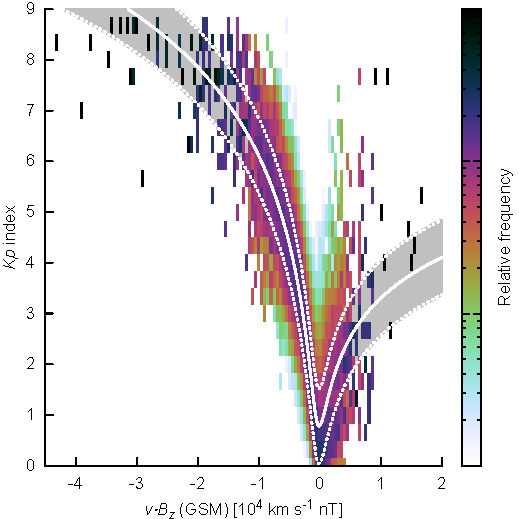
\includegraphics[width=\textwidth]{figures_of_mine/gnuplots/KpvsBz_titlepage.pdf}
\end{minipage}
\begin{minipage}{0.08\textwidth}
\end{minipage}
\begin{minipage}{0.46\textwidth}
	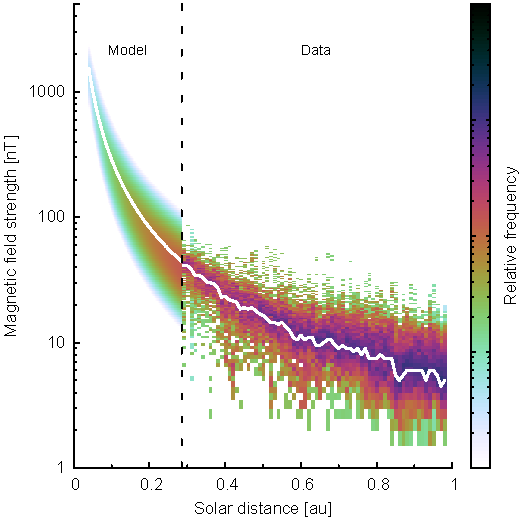
\includegraphics[width=\textwidth]{figures_of_mine/gnuplots/fit_fixed_B_paper_f_title.pdf}
\end{minipage}

% \begin{figure}[htb]
% 	\centering
% 	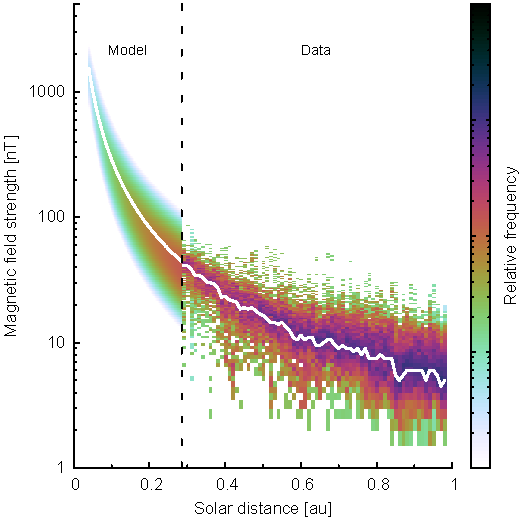
\includegraphics[width=0.46\textwidth]{figures_of_mine/gnuplots/fit_fixed_B_paper_f_title.pdf}
% 	\caption[\lofimage{figures_of_mine/gnuplots/fit_fixed_B_paper_f_title.pdf}]
% 	{Combined figure of \autoref{fig:fit_fixed_B_paper_f}.}
% 	\label{fig:fit_fixed_B_paper_f_title}
% \end{figure}
% 
% % figure notes
% see \autoref{fig:fit_fixed_B_paper_f_title}\\


% electronic version note
\begin{small}
	\noindent The electronic version of this document is fully hyperlinked. The external links in some figure captions and in the references are not accessible in the printed version. All external web links in this document were valid in 2018-XX-XX.
\end{small}

\vfill

\begin{footnotesize}
\noindent version log:\\
1	2013-11-06\\
2	2013-11-07	inserted lem excerpt\\
3	2014-09-01	outlined introduction structure and appendix key words\\
4	2014-09-11	bibtex included, lem excerpt citet\\
5	2014-09-12	included italic titles in bibliography\\
6	2015-01-12	worked on introduction structure and included magnetic butterfly diagram\\
7	2015-05-04	first printout, small additions\\
8	2015-07-03	coupling functions, content structure\\
9	2015-09-09	Alfv\'en wave velocity formula\\
10	2015-09-10	Appendix physics: Alfv\'en and compressional MHD waves, plasma beta; citation sources Cranmer2005, Kivelson1995\\
% 11	2015-09-15	CGAUSS work overview; DQCS model figure\\
% 12	2015-09-16	magnetic energy density is the same as magnetic pressure, abbreviations\\
% 13	2015-09-30	empirical solar wind model plots in analyses, figure label [Figure 4.2  Text]\\
% 14	2015-10-02	table column decimal alignment; set caption width\\
% 15	2015-10-05	table units; radial parameter (N, T) profiles in literature\\
% 16	2015-10-06	literature radial electron density models; log-normal distribution\\
% 17	2015-10-07	log-normal formulae\\
% 18	2015-10-08	log-normal fit\\
% 19	2015-10-09	shape fit parameter table; radial variance fitting\\
20	2015-10-14	variance fit values; log-normal citation Bronstein\\
% 21	2015-10-19	radial distribution width fitting; clarifying of solar wind model formulae structure and naming variables\\
% 22	2015-10-20	log-normal distribution width factor changes the shape!\\
% 23	2015-10-23	log-normal distributions mu and sigma plot\\
% 24	2015-10-30	new sigmafit2 figures implemented; formulae adaption\\
% 25	2015-11-02	reason for use of log-normal function\\
% 26	2015-11-20	single log-normal shape fit; not chisquare - SSR; $R^2$ in appendix\\
% 27	2015-11-26	reduced SSR into tables; table column aligning\\
% 28	2015-12-02	smoothing SSR integration\\
% 29	2015-12-07	integrating structure remarks from printout\\
30	2015-12-09	splitting analyses chapter into two; browsing folders for usable things for thesis\\
% 31	2015-12-10	integrating citations and references\\
% 32	2015-12-16	integrating citations and references\\
% 33	2015-12-18	solar wind structures list of Richardson\\
% 34	2016-02-02	sws distributions\\
% 35	2016-02-11	basics structure\\
% 36	2016-02-12	analyses questions\\
% 37	2016-02-15	analyses structure; in situ, near-Sun\\
% 38	2016-02-16	Kp index internal resolution\\
% 39	2016-02-17	Bartels1962; non-breaking hyphen shorthand implemented\\
40	2016-02-18	analysesI structure\\
% 41	2016-02-25	abstract\\
% 42	2016-02-26	english comma\\
% 43	2016-03-01	Bartels Kp origin paper, bibtex reference\\
% 44	2016-03-02	abstract\\
% 45	2016-03-03	Planck paper\\
% 46	2016-03-07	formation of stars\\
% 47	2016-03-08	formation of stars\\
% 48	2016-03-16	solar interior structure\\
% 49	2016-03-17	solar interior structure\\
50	2016-03-18	solar surface\\
% 51	2016-03-22	Astronomical Almanac citation\\
% 52	2016-03-23	solar core definition\\
% 53	2016-03-26	sunspots\\
% 54	2016-03-29	Sun interior figure\\
% 55	2016-03-30	solar composition\\
% 56	2016-03-31	Sun interior figure finished; chromosphere\\
% 57	2016-04-01	Sun atmosphere figure finished\\
% 58	2016-04-03	chromosphere, corona, CV\\
% 59	2016-04-07	CV\\
% 60	2016-04-08	CV; heliosphere\\
% 61	2016-04-09	corona; heliosphere\\
% 62	2016-04-11	heliosheath magnetic bubbles; Opher2011\\
% 63	2016-04-12	heliosphere; voyagers; Gurnett2013\\
% 64	2016-04-13	solar wind effects, solar rotation\\
65	2016-04-14	analysesI sws structure draft plots\\
% 66	2016-04-15	analysesI concept work\\
% 67	2016-04-19	incorporate annotations from processed printout\\
% 68	2016-04-21	incorporate annotations from processed printout II\\
% 69	2016-04-22	incorporate annotations from processed printout III\\
% 69	2016-04-23	updated .bst file (for displaying arXiv id); implemented optional url displaying for electronic version; Kp year variations\\
% 70	2016-04-24	Kp frequency by month statistics and plot; Sun and Earth tilt plot\\
% 71	2016-04-25	solar cycle extrema dates literature\\
% 72	2016-04-27	Kp semi annual variation, Rangarajan1997\\
% 73	2016-05-01	Kp frequency by year\\
% 74	2016-05-04	Kp + SSN plot; ACE data errors/gaps; log-normal plot; differential rotation plot\\
% 75	2016-05-05	aggregate correlation coefficient tables, CME fraction plot\\
% 76	2016-05-06	overall sws fractions\\
% 77	2016-05-17	figure sw frequencies by year; restructured solar wind distributions section; formal cover page\\
% 78	2016-05-20	Earth-Sun distance; JPL web interface\\
% 79	2016-05-31	GSM system\\
80	2016-06-10	Offline Anmerkungen einarbeiten\\
% 81	2016-06-12	LaTeX Earth symbol package\\
% 82	2016-06-13	numbers=noenddot\\
% 83	2016-06-14	references removed comma before ampersand; offline Anmerkungen einarbeiten; thesis\_raw version\\
% 84	2016-06-17	gnuplot figures and latex; latex document style options\\
% 85	2016-06-19	header implemented\\
% 86	2016-06-20	minor things; introduction\\
% 87	2016-06-23	solar tilt axis\\
% 88	2016-06-24	solar rotation\\
% 89	2016-07-12	magnetosphere temp figure; analyses: solar wind model\\
% 90	2016-07-13	lognormal spelling\\
% 91	2016-07-14	constant mass flow rate\\
% 92	2016-07-18	line-up periods\\
% 93	2016-07-19	line-up periods table\\
% 94	2016-07-20	redone line-up analysis\\
% 95	2016-07-21	line-up tables\\
% 96	2016-07-22	line-up fit function plots; coefficient table\\
% 97	2016-07-22	line-up sw types and period plots; overview plot\\
% 98	2016-07-24	line-up averaging and justification\\
% 99	2016-07-29	line-up rework\\
100	2016-07-30	line-up structure\\
% 101	2016-07-31	line-up table\\
% 102	2016-08-02	line-up structure\\
% 103	2016-08-03	line-up fits and table\\
% 104	2016-08-04	insert offline comments\\
% 105	2016-08-15	literature radial sw functions\\
% 106	2016-08-18	work offline comments in\\
% 107	2016-08-19	work offline comments in\\
% 108	2016-08-28	analyses II rework structure\\
% 109	2016-08-31	analyses II rework structure\\
% 110	2016-09-01	analyses II rework figures\\
% 111	2016-09-02	analyses II rework structure\\
% 112	2016-09-03	Helios latitude dependency\\
% 113	2016-09-04	extrapolation model fit parameter table; Helios latitude dependence\\
% 114	2016-09-06	work in offline comments\\
% 115	2016-09-14	implement median and mean in composite fit table; create kile project for thesis; url and raw fork\\
% 116	2016-09-17	Ulysses polar plot; solar distance plots\\
% 117	2016-09-18	for solar distance and latitude -> 4-panel figures created and implemented; appendix figures\\
% 118	2016-09-20	latitude plots updated\\
% 119	2016-09-26	single lognormal fit figure\\
120	2016-09-27	minor tweaks in analyses II\\
% 121	2016-09-29	simple fit table errors; table style\\
% 122	2016-10-05	lognormal fit errors for tables\\
% 123	2016-10-10	line-up passing remarks from AP\\
% 124	2016-10-12	siunitx package incorporated\\
% 125	2017-01-04	package fancyhdr replaced with scrlayer-scrpage; offline comments for Basics + Data incorporated\\
% 126	2017-01-06	package floatrow included for figure side captions; some cites; magnetometer\\
% 127	2017-01-08	sun figure updates and new ion energy spectrum figure incorporated\\
% 128	2017-01-13	offline comments, new chapter order\\
% 129	2017-01-18	activated hyperref package; included autoref and eqref; adjusted link colors; header links\\
% 130	2017-02-02	offline commtents\\
% 131	2017-02-03	offline commtents II, eclipse image\\
% 132	2017-02-06	basics figures with floatrow; flow structure\\
% 133	2017-02-07	ion energy spectrum figure\\
% 134	2017-02-09	Helios mission ssn plot\\
% 135	2017-02-12	offline comments\\
% 136	2017-02-13	section number link to toc; offline comments\\
% 137	2017-02-14	eclipse and magbfly figure captions\\
% 138	2017-02-16	offline comments\\
% 139	2017-02-19	coronal heating and sw acceleration\\
140	2017-04-22	set up git repository\\
% 141	2017-04-23	incorporate offline comments\\
% 142	2017-04-26	bipolar region draft\\
% 143	2017-04-27	magnetic layer Ossendrijver2003\\
% 144	2017-06-29	magnetosphere figure drafts implemented\\
% 145	2017-07-16	streamlined content - including paper and chapter2\\
% 146	2017-07-22	streamlined duplicate content\\
% 147	2017-10-05	Kp index data\\
% 148	2017-10-28	geomagnetic indices; Kp index; Kp to ap table\\
% 149	2017-10-29	Kp index\\
% 150	2017-10-30	OMNI s/c coverage figure\\
% 151	2017-10-31	OMNI s/c coverage figure upgrade; data set timeline figure\\
% 152	2017-11-01	SSN prediction; omega-effect\\
% 153	2017-11-02	alpha-omega dynamo; magnetogram figure upgrade\\
% 154	2017-11-03	worked on figure permissions; alpha-omega-figure\\
% 155	2017-11-04	paperMVVB inserted; worked on compatibility\\
% 156	2017-11-12	paperMVVB: figure size, tablefoot, adjusted table width; included chapter2; ordered file implementing\\
% 157	2017-11-14	figure permission Babaszkiewicz1998\\
% 158	2017-11-15	poking around in image credits; solar activity cycle\\
% 159	2017-11-16	solar activity cycle; Zhao image permission\\
160	2017-11-17	Zhao copyright symbol included; solar wind; commata and sentence wording\\
% 161	2017-11-22	notes from github paper folder\\
% 162	2017-11-23	Ulysses figure permission and caption; pdfpages package; paper included as is\\
% 163	2017-11-24	GUM reference; Helios data frequency figure\\
% 164	2017-11-25	intro to paper\\
% 165	2017-11-26	intro to paper\\
% 167	2017-11-27	Cranmer2005 fig1; Banaszkiewicz fig\\
% 168	2017-11-28	HCS and Parker spiral\\
% 169	2017-11-29	heliosheath; Cranmer2005 permission\\
% 170	2017-11-30	chapter2 updated\\
% 171	2017-12-06	upgraded: title, abstract, introduction, basics outline, notes to chapter2; worked in offline comments until HMF\\
% 172	2017-12-08	MBPs; Solar wind section structure\\
% 173	2017-12-10	solar wind basics, draft figs for CIR and CME\\
% 174	2017-12-11	draft figs for COR2 CME and ACE MC; solar wind history\\
% 175	2017-12-13	B-field improvement\\
% 176	2017-12-14	B-field improvement \#2\\
% 177	2017-12-15	B-field improvement \#3\\
% 178	2017-12-16	B-field angles plot\\
% 179	2017-12-17	B-field improvement \#4\\
180	2017-12-21	B-field: four plots upgraded\\
% 181	2017-12-31	B-field: worked offline comments in; included chapter2 update\\
% 182	2018-01-01	autoref names; solar wind properties; literature\\
% 183	2018-01-02	sw helium share; plasma beta; source surface; mass flux considerations\\
% 184	2018-01-04	sw considerations; fast/slow wind\\
% 185	2018-01-05	fig Hundhausen; fast slow sw\\
% 186	2018-01-08	fast slow sw\\
% 187	2018-01-09	slow sw sources\\
% 188	2018-01-10	slow sw; slow/fast cycle pattern\\
% 189	2018-01-11	Wang1990\\
% 190	2018-01-14	HCS and SIR\\
% 191	2018-01-15	HCS + CIR\\
% 192	2018-01-16	in-situ event plots\\
% 193	2018-01-17	in-situ CIR/HSS plot\\
% 194	2018-01-19	CME/MC plot; VB comments\\
% 195	2018-01-20	VB comments...\\
% 196	2018-01-21	VB comments; Alfvén waves\\
% 197	2018-01-22	VB comments; removed line-up study; merged appendix; removed unused tex and image files\\
% 198	2018-01-24	HMF offline comments\\
% 199	2018-01-26	B improvement offline comments; APL PSP pictures; adjust pdfinfo\\
200	2018-01-28	chapter2 implemented into thesis; figure folders rearranged; figures floatrow implemented\\
% 201	2018-01-29	abstract updated; contents structure streamlined\\
% 202	2018-01-29b	instrumentation and data sources\\
% 203	2018-01-30	OMNI and Helios data\\
% 204	2018-01-31	chapter2 R-M effect literature\\
% 205	2018-01-31b	R-M effect literature; chapter2 coupling into basics\\
% 206	2018-02-01	formal titlepage\\
% 207	2018-02-03	front matter; pdf toc bookmarks\\
% 208	2018-02-05	sw in-situ fig\\
% 209	2018-02-06	SIRs\\
% 210	2018-02-07	SIRs II\\
% 211	2018-02-09	CMEs\\
% 212	2018-02-11	CMEs II\\
% 213	2018-02-11b	CMEs IIb\\
% 214	2018-02-12	CMEs III\\
% 215	2018-02-13	CMEs IV\\
% 216	2018-02-14	CMEs V\\
% 217	2018-02-15	CMEs VI\\
% 218	2018-02-16	CME images...\\
% 219	2018-02-19	HCS into HMF\\
220	2018-02-20	HCS in sw section\\
% 221	2018-02-21	work in offline comments\\
% 222	2018-02-23	work in offline comments II\\
% 223	2018-02-25	CMEs; CMEs.tex\\
% 224	2018-02-26	CMEs.tex II\\
% 225	2018-02-27	CMEs.tex III\\
% 226	2018-02-28	figure captions - removed explanations\\
% 227	2018-03-01	figure permissions documentation 80\%\\
% 228	2018-03-02	figure permissions list - remove caption before credits; CMEs.tex IV\\
% 229	2018-03-03	CMEs.tex V\\
% 230	2018-03-04	CMEs.tex VI, BSS\\
% 231	2018-03-04b	CMEs.tex VI, MC figure\\
% 232	2018-03-05	CMEs.tex VII, CBS\\
% 233	2018-03-05b	CMEs.tex VIIb, 3D models\\
% 234	2018-03-06	CMEs, figures\\
% 235	2018-03-07	CMEs, figures, fig. captions\\
% 236	2018-03-08	CMEs.\\
% 237	2018-03-09	CMEs..\\
% 238	2018-03-10	figure permission hundhausen1977\\
% 239	2018-03-13	CME formation\\
240	2018-03-16	chapter2 offline corrections implemented\\
% 241	2018-03-17	chapter2 fit curves figure; sw example plot vBz figure\\
% 242	2018-03-19	chapter2 sw example plot v figure; and figure captions\\
% 243	2018-03-20	new paper pdf; references link shortcuts\\
% 244	2018-03-21	chapter2 SSN 300 plots corrected; error sizes; quantiles added; CME offline corrections\\
% 245	2018-03-22	CME offline corrections; magnetosphere figure...\\
% 246	2018-03-25	last CME offline corrections; paper B-field addendum offline corrections\\
% 247	2018-03-26	CME formation; space weather\\
% 248	2018-03-28	stuff from Cranmer2017, Savani2015+2017\\
% 249	2018-03-29	magnetosphere figure implemented\\
% 250	2018-03-31	Adams comments for PSP chapter; sectioning space weather + magnetosphere\\
% 251	2018-04-01	magnetosphere 2D and 3D figures; DeKeyser2005 + Phan2005; Dungey1963\\
% 252	2018-04-03	space\_weather.txt 1--3\\
% 253	2018-04-04	space\_weather.txt 4\\
% 254	2018-04-05	electronic version note; space\_weather.txt implemented; excerpts sorted\\
% 255	2018-04-06	Dungey cycle\\
% 256	2018-04-06b	Summary\\
% 257	2018-04-07	magnetosphere sorting\\
% 258	2018-04-09	space weather\\
% 259	2018-04-10	space weather 2; magnetosphere\\
260	2018-04-11	magnetosphere 3; reconnection figure\\
% 261	2018-04-16	CMEs; showoff version created\\
% 262	2018-04-16b	title figure 2\\
% 263	2018-04-19	space weather offline comments incorporated\\
% 264	2018-04-20	coupling mechanisms\\
% 265	2018-04-21	coupling mechanisms; turbulence\\
% 266	2018-04-22	Dungey cycle\\
% 267	2018-04-23	Dungey cycle 2\\
% 268	2018-04-24	Dungey cycle 3\\
% 269	2018-04-25	Dungey cycle 4\\
% 270	2018-04-25b	R-M effect\\
% 271	2018-04-26	R-M effect 2\\
% 272	2018-04-26b	geomagnetic storms\\
% 273	2018-04-30	geomagnetic storms 2\\
% 274	2018-05-01	offline comments s/w; stream kp-sw plot\\
% 275	2018-05-02	geomagnetic storms 3\\
% 276	2018-05-03	geomagnetic storms 4; Dst index\\
% 277	2018-05-04	not really\\
% 278	2018-05-05	Birkeland current system\\
% 279	2018-05-07	offline comments implemented\\
280	2018-05-08	kp index\\
% 281	2018-05-09	minor changes\\
% 282	2018-05-09	Geomagnetic activity forecast; E = -vBz\\
% 283	2018-05-10	E = -vBz\\
% 284	2018-05-11	coupling functions; Newell function\\
% 285	2018-05-12	coupling functions\\
% 286	2018-05-13	coupling functions 3\\
% 287	2018-05-14	coupling functions 4\\
% 288	2018-05-17	implementing offline comments: coupling functions\\
% 289	2018-05-30	coupling functions 5\\
% 290	2018-05-31	Kp forecast\\
% 291	2018-06-01	implementing offline comments: Kp forecast\\
% 292	2018-06-02	implementing offline comments 2: coupling functions\\
% 293	2018-06-03	Kp empirical functions\\
% 294	2018-06-04	Kp empirical functions 2\\
% 295	2018-06-05	Wing Kp model\\
% 296	2018-06-07	prediction performance and true skill score\\
% 297	2018-06-10	appendix: true skill statistics\\
% 298	2018-06-11	appendix: true skill statistics; Kp persistence\\
% 299	2018-06-12	chapter2: prediction performance, TSS, statistics table\\
300	2018-06-13	chapter2: TSS\\
% 301	2018-06-14	Kp forecast models\\
% 302	2018-06-16	comments Adam + VB\\
% 303	2018-06-17	comments VB\\
% 304	2018-06-17b	comments VB 2\\
% 305	2018-06-18	comments VB 3\\
% 306	2018-06-19	Kp forecast; CME forecast\\
% 307	2018-06-20	Kp prediction models\\
% 308	2018-06-21	magnetometer\\
% 309	2018-06-22	sw forecast to Earth\\
% 310	2018-06-23	acknowledgements; coordinate systems\\
% 311	2018-06-25	coordinate systems\\
% 312	2018-06-26	magnetometer; plasma detector\\
% 313	2018-06-27	lognormal distribution; Sun-Earth geometry\\
% 314	2018-06-27b	Sun-Earth geometry plot; solar distance\\
% 315	2018-06-28	Sun-Earth geometry 2\\
% 316	2018-06-28b	plasma detector 2\\
% 317	2018-06-29	solar differential rotation\\
% 318	2018-06-29b	solar differential rotation 3\\
% 319	2018-06-30	sw stream and CME forecast to Earth\\
320	2018-06-30b	sw stream and CME forecast to Earth 2\\
% 321	2018-07-01	looking through chapter2 until 4.3\\
% 322	2018-07-01b	looking through chapter2 until 4.3.2; E-field at the magnetopause\\
% 323	2018-07-02	looking through chapter2 until 4.3.3\\
% 324	2018-07-02b	looking through chapter2 until 4.4\\
% 325	2018-07-04	offline comments implemented\\
% 326	2018-07-04b	offline comments implemented 2\\
% 327	2018-07-05	last offline comments, CME forecast\\
% 328	2018-07-09	data links into text; CME forecast 2\\
% 329	2018-07-10	solar wind nowcast; looking through chapter2 until 4.4.1\\
% 330	2018-07-11	looking through chapter2 until 4.4.3\\
% 331	2018-07-12	looking through chapter2\\
% 332	2018-07-13	PSP mission\\
% 333	2018-07-14	introduction\\
% 334	2018-07-16	implement offline comments\\
% 335	2018-07-17	PSP mission 2; acronyms\\
% 336	2018-07-19	english titlepage; tabular CV; minor things\\
% 337	2018-07-20	acronyms into two columns; chapterPSP\\
% 338	2018-07-21	chapterPSP; figure: IMF comparison\\
% 339	2018-07-22	chapterPSP\\
340	2018-07-22b	chapterPSP discussion\\
% 341	2018-07-23	basics intro; introduction synopsis\\
% 342	2018-07-25	implement offline comments chapterPSP; tabular CV\\
% 343	2018-07-25b	acknowledgments\\
% 344	2018-07-28	implement offline comments chapter2\\
345	2018-07-28b	implement offline comments chapter2 2; summary handout\\
% 346	2018-07-29	implement offline comments appendix ff.\\
% 347	2018-07-30	abstract page\\
% 348	2018-07-30b	introduction\\
% 349	2018-07-31	introduction 2\\
350	2018-08-01	data acknowledgments\\
351	2018-08-01b	introduction 3\\
352	2018-08-02	introduction 4\\
353	2018-08-03	introduction 5\\
354	2018-08-05	introduction 6\\
355	2018-08-06	new title; conclusions\\
356	2018-08-08	implement offline comments chapter2\\
357	2018-08-09	implement offline comments chapter2 2\\
\vspace{\baselineskip}
\ISOToday{} \thistime{} -- last save
\end{footnotesize}


\clearpage


\vspace*{\fill}

%Zitat in Diplomarbeit:
%\textit{"[...], und während er sich solchermaßen in der unteren Region des Reiches der Wissenschaft bewegte, dort, wo dieses unmerklich in das Reich der Psychiater übergeht, eignete er sich schließlich doch eine ganze Menge durchaus nützlicher Kenntnisse an, [...]"}
%denn er wusste immer erstaunlich gut Bescheid,
%\noindent Zitat: Stanislaw Lem, "Die Stimme des Herrn", S.56.

\noindent \textit{``Despite the `Dr.' before his name, he had completed no course of study and received no degree. When people tried to pin him down about this, he would say that the letters were merely an abbreviation of his first name - Drummond - which he did not use. But it was as `Dr.' Sam Laserowitz that he appeared in a number of science-fiction magazines; he was also known, in the circles of the fans of that genre, as a lecturer, and spoke on `cosmic' themes at their many conferences and convention. Laserowitz's speciality was earthshaking discoveries, wich he happened upon two or three times a year. [...] We really have no idea what a multitude of con men and crackpots inhabit the domain that lies halfway between contemporary science and the insane asylum.''}
\vspace{\baselineskip}

\noindent Excerpt from Stanis\l aw Lem 1968, \textit{His Master's Voice} \citep[p.~38]{Lem1984}.
%quote vs quotation vs excerpt

\vspace{\stretch{4}}

\newpage

\begin{abstract}
	\section*{Abstract}	%or abstract=true
	\noindent This thesis derives empirical predictions of the solar wind's impact on the terrestrial magnetosphere and of the solar wind environment in the near-Sun region.
	%magnetosphere impact
	Near-Earth in-situ solar wind measurements, consisting of 35~years of minutely OMNI data, are analyzed together with the time series of the planetary geomagnetic disturbance indicator \Kp{}. Correlations and functional dependencies are compiled with regard to nowcast the magnitude of the geomagnetic disturbances from in-situ solar wind measurements and to forecast them from remotely observed solar wind streams and coronal mass ejections.
	%solar activity
	Further, 53~years of hourly OMNI data and sunspot number data are correlated for the purpose of deriving functional dependencies with the state of the solar cycle for the key solar wind parameters magnetic field strength, proton velocity, density, and temperature.
	%solar distance
	Solar wind in-situ data from the Helios~1 and~2 missions, operational in the 1970s and orbiting the Sun within the distance range \SIrange{0.3}{1.0}{\au}, are analyzed and empirical solar wind distance dependencies are derived. Additionally, in view of the near-Sun spacecraft mission Parker~Solar~Probe which launched in mid~2018, the solar wind environment is estimated down to its closest perihelion at \num{9.86}~solar radii.
% 	use
	The empirical solar wind and \Kp{} relations derived in this work provide useful tools for estimating the corresponding quantities. The relations are especially valuable within the scope of space weather predictions.
\end{abstract}

% \noindent Key words: solar wind -- coronal mass ejections (CMEs) -- solar-terrestrial relations -- magnetosphere -- \Kp~index -- inner heliosphere -- Parker Solar Probe (PSP)

\newpage

%\cleardoublepage
%\tableofcontents
\pdfbookmark[0]{Contents}{toc_pdf_bookmark}
{\let\cleardoublepage\clearpage\tableofcontents}	%open contents on left page
\label{sec:toc}
\cleardoublepage
%\listoffigures
%\listoftables


	\pagenumbering{arabic}
	\chapter{Introduction}
\label{chap:introduction}

Introductory text -> Motivation for\\
- time variation analysis\\
- distance analysis\\
- Kp impact analysis\\
%(Kurzer Text zur Motivation für diese Arbeit, wie das Ziel erreicht wurde und wie es zum Thema kam.)

% Questions this work asks:\\	%Fragestellungen ausformuliert
% 	How strong is the solar wind influence on the terrestrial magnetosphere?\\
% 	How often occur certain solar wind ranges?\\
% 	How strong do different structure types influence the terrestrial magnetosphere?\\
% forecast:\\
% 	How can the impact strength of the solar wind be forecasted? (VBz->Kp L1-Alerts)\\
% 	How can the impact strength of CMEs be forecasted (V->Kp correlation for CMEs)?\\
% 	(How can the impact field strength of CMEs be forecasted (V->B correlation for CMEs)?)\\

% 	How does the solar wind evolve on its way from the Sun?\\
% 	How do the different structures evolve on their way from the Sun?\\
% 	What are the properties of the solar wind near the Sun?\\
% 	(Where does the solar wind get accelerated?)\\
% 	(How does the solar wind get accelerated?)\\
% 	(How is this related to the coronal heating problem?)\\

%Outline of this thesis:
Synopsis (chapters, content)\\	%Gliederung der Arbeit (zum Schluss ueberarbeiten)
This thesis merges the solar wind analyses of its variation in time (autoref{}), its evolution to Earth (Chapter~XX) and its impact on the magnetosphere (Chapter~XX). Lists of constants, symbols and abbreviations used in this thesis are located in the appendix.\\


\chapter{Basics}
\label{chap:basics}

%COFI -- chapter outline and flow integration\\
First this chapter sketches the Sun's origin, inner structure, atmosphere and heliosphere. Then the Sun's dynamics with its magnetic field variations and solar cycle are outlined (including differential rotation, magnetic field generation, solar cycle, quiet/active Sun characteristics on surface and solar wind with HMF consequences). The solar wind and its characteristic structures are described. Further, the solar influence on Earth, on its magnetosphere and other space weather effects are portrayed.\\
%first the existing structures, second their dynamics, last their influence on humans/their technology (space weather)


\section{Solar composition}
\label{sec:solar_composition}

%%% universe
13.8~billion years ago the Big~Bang formed our universe. The energy density of our universe consists of \SI{69.1}{\percent} dark energy, \SI{25.9}{\percent} dark matter and \SI{4.9}{\percent} baryonic matter according to calculations using the inflationary $\Lambda$CDM cosmology together with the latest CMB temperature measurements \citep{Planck2016}.
%see Planck2016 page 31 Table 4		age of universe
%see Planck2016 page 31 Table 4 and en.wikipedia.org/wiki/Lambda-CDM_model#Parameters
%energy density consists of
%dark energy $\Omega_\Lambda = 0.6911$,
%matter $\Omega_\text{m} = 0.3089$,
%dark matter $\Omega_\text{c} = 0.2589$ and
%baryonic matter $\Omega_\text{b} = 0.0486$
After a few minutes the primordial nucleosynthesis left the universe in a state where the baryonic matter was composed of \SI{75.33}{\percent}\footnote{Percentages by mass.} hydrogen, \SI{24.67}{\percent} helium and traces of deuterium, tritium and lithium \citep{Planck2016}.
%see Planck2016 page 47 Eq. 73

%%% star formation
Over the years this gas cooled down and gravitationally accreted into molecular clouds and formed stars. The first generations of stars (Population~III) fused this gas to heavier elements (metals) and supernovae distributed them into space as a foundation for the formation of new stars of low and high metallicity (Population~II and I). Likewise, supernovae of these stars constantly enriched the interstellar medium with metals. Now, the interstellar medium in the Milky~Way consists of about \SI{32}{\percent} helium and traces of other metals \citep{Danziger1970}.\\
%In 20XX the Voyager~? probe measured a density of about ...\SI{0}{\per\cm\cubed} right outside of the heliopause (cite?).\\

%%% solar interior
Our Sun, a metal-rich Population~I yellow dwarf star, emerged 4.6~billion years ago \citep{Bahcall1995} from an accretion disk formed by a collapsing rotating cloud. The compression within its center resulted in high temperatures which initiated the fusion of hydrogen to helium (primarily pp~chain reaction). The fusion reactions produce huge amounts of energy and heat the solar center to a temperature of 15.7~million~kelvins \citep{Christensen-Dalsgaard1996}. The generated energy is transported through the solar body to its surface and eventually into space.
The core region extends to about 0.25~solar radii (\Rsun), where the declining temperature becomes insufficient for fusion reactions. The energy transport is dominated by thermal radiation until, because of declining ionization and density, at 0.71\,\Rsun{} up to the surface convective motion takes over \citep{Christensen-Dalsgaard1991}. %0.7: http://adsabs.harvard.edu/abs/1991ApJ...378..413C
%Dalsgaard Model S: http://astro.phys.au.dk/~jcd/solar_models/
%core radius (cite?)

%%% photoshere + sunspots
The temperature at this transition region (tachocline) is about 2~million~kelvins and decreases up to the solar surface to between \SIrange{4400}{6600}{\K} (cite?). Here at the photosphere, the energy is radiated away with an effective black body temperature of \SI{5772}{\K} \citep{Mamajek2015}, classifying the Sun as a spectral type G2V star.
At this surface layer granules, the tops of convection cells, and temporary sunspots are visible. Strong magnetic flux inhibits the convection at sunspots, leading to lower temperature and brightness (for more details on sunspots see Section~XX...). \autoref{fig:sun_interior_HMIIC} illustrates these photospheric features along with the inner solar structure.\\
\begin{figure}[htb]
	%\centering
	\fcapside[\FBwidth]{
		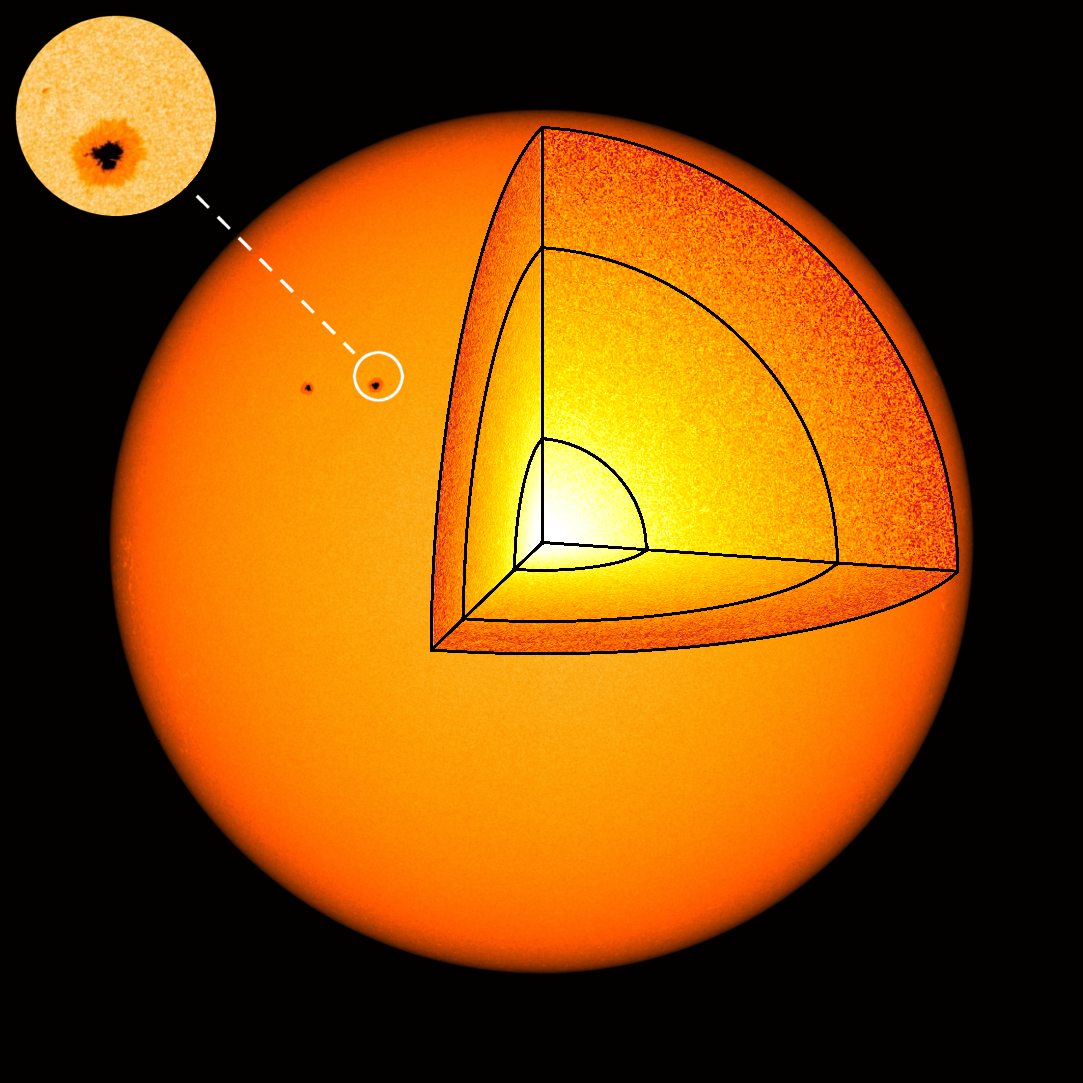
\includegraphics[width=0.6\textwidth]{images/own_figures/sun_interior_HMIIC.png}
	}{
		\caption{Image of the photosphere together with a schema of the solar interior structure. The inset shows the granular surface with a sunspot. The figure is based on a SDO/HMI continuum image from 20~March~2016; credit: NASA/SDO and the AIA, EVE and HMI science teams.}
		\label{fig:sun_interior_HMIIC}
	}
\end{figure}

%%% chromosphere + corona + CMEs
Above the photosphere at the base of the chromosphere the temperature declines to its solar minimum of \SI{3800}{\K} until it raises to \numrange{1}{3}~million~kelvins in the corona (cite? 2.4~GK Billings1959). Up to now it is not fully understood why the corona is so much hotter than the underlying chromosphere---this question is known as the coronal heating problem (cite?). The energy transfer mechanisms of choice are magnetic reconnections, wave heating and type~II spicules or a combination of these.

The chromosphere is a \SI{2000}{\km} thick region whose features (numerous spicules, filaments and prominences) can range far into the corona. They consist of by the solar magnetic field channeled chromospheric material, which is enveloped by a thin transition region where the temperature jumps up from ?\SIrange{20000}{35000}{\K} to coronal temperatures (cite?). Reconnection of magnetic field lines can result in the eruption of filaments into the corona and beyond, termed coronal mass ejections (CMEs) (see also Section~XX...). Details of chromospheric features are shown in \autoref{fig:sun_atmosphere}.

%%% coronal holes
The Sun's atmosphere is dominated by the varying small- and large-scale solar magnetic field configuration. There are regions where the magnetic field lines arc back to the surface and regions with open field lines. In the latter areas the coronal plasma can---guided by the field---escape into space. Thus these coronal areas are less dense, cooler and therefore appear darker in extreme ultraviolet (EUV) and are called coronal holes (more in Section~XX...). In \autoref{fig:sun_atmosphere} a coronal hole is located at the solar south pole.
\begin{figure}[htb]
	%\centering
	\fcapside[\FBwidth]{
		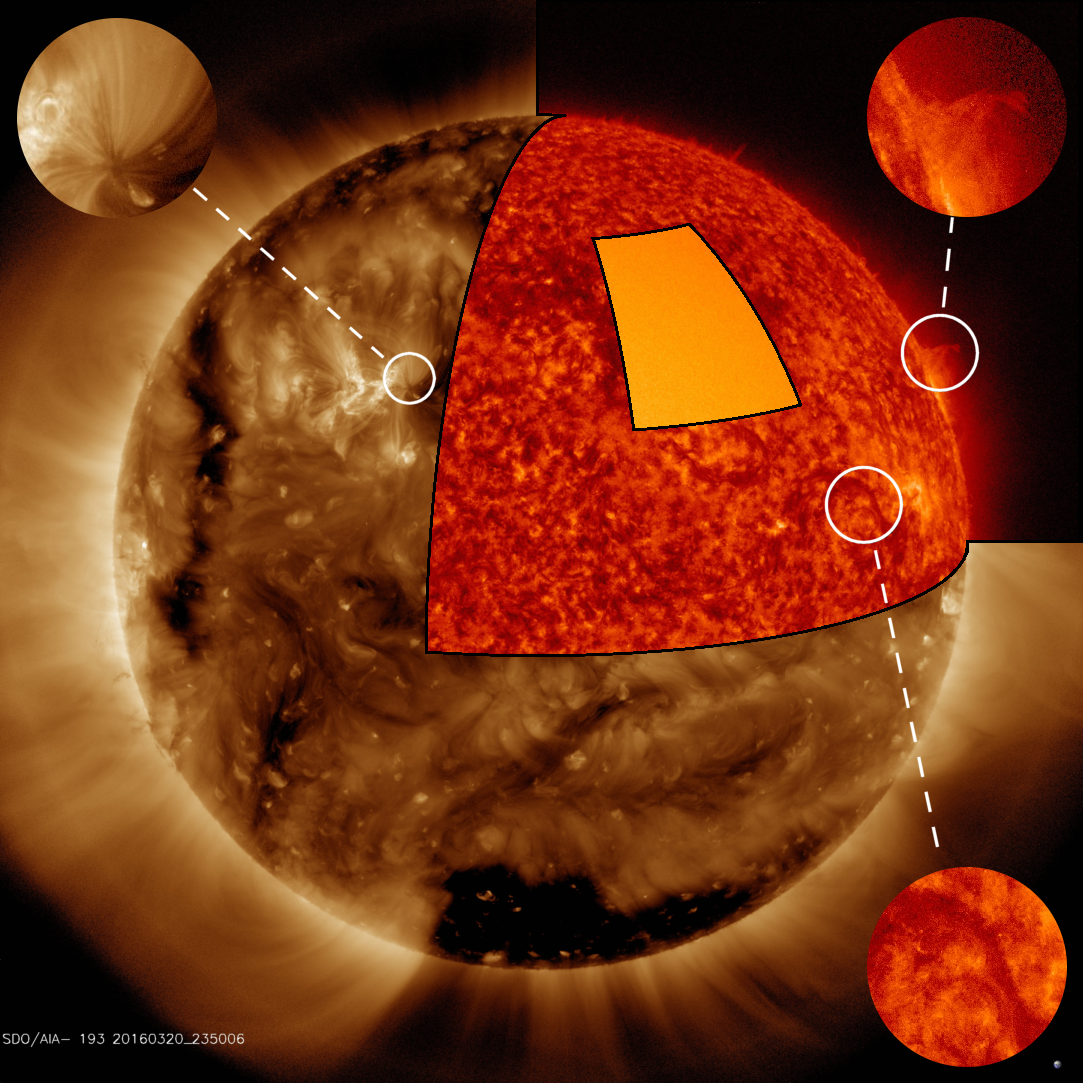
\includegraphics[width=0.6\textwidth]{images/own_figures/sun_atmosphere.png}
	}{
		\caption{Composite image of the solar atmosphere and some of its features. Corona, chromosphere and photosphere are seen in wavelengths of \SI{193}{\angstrom}, \SI{304}{\angstrom} and continu\-um. On the northern limb chromospheric spicules are visible. The enlargements on the right show a prominence and a filament. The dark region at the south pole is a coronal hole. The left inset shows details of the active region belonging to the sunspots in \autoref{fig:sun_interior_HMIIC}. The figure is based on SDO/AIA images from 20~March~2016; credit: NASA/SDO and the AIA, EVE and HMI science teams.}
		\label{fig:sun_atmosphere}
	}
\end{figure}

%%% corona
From Earth the faint corona and chromosphere can only be observed during eclipses, because of the brightness of the solar disk. There are three effects contributing to the visibility of the corona, photon scattering off free electrons and dust particles, and ion spectral emission lines (K-, F- and E"~corona).
% the so-called K-, F- and E"~corona (K kontinuierlich, F Fraunhofer, E emission).\\
% K-corona: photon scattering off free electrons --> coronagraphs\\
% F-corona: photon scattering off dust particles; contains Fraunhofer absorption lines; expands in ecliptic as zodiacal light --> coronagraphs\\
% E-corona: ion spectral emission lines; reveals coronal composition --> images\\
The image of a solar eclipse reveals the by the magnetic field shaped coronal plasma and features of the red chromosphere, pictured in \autoref{fig:Tse2008_500_mo1}.\\
\begin{figure}[htb]
	%\centering
	\fcapside[\FBwidth]{
		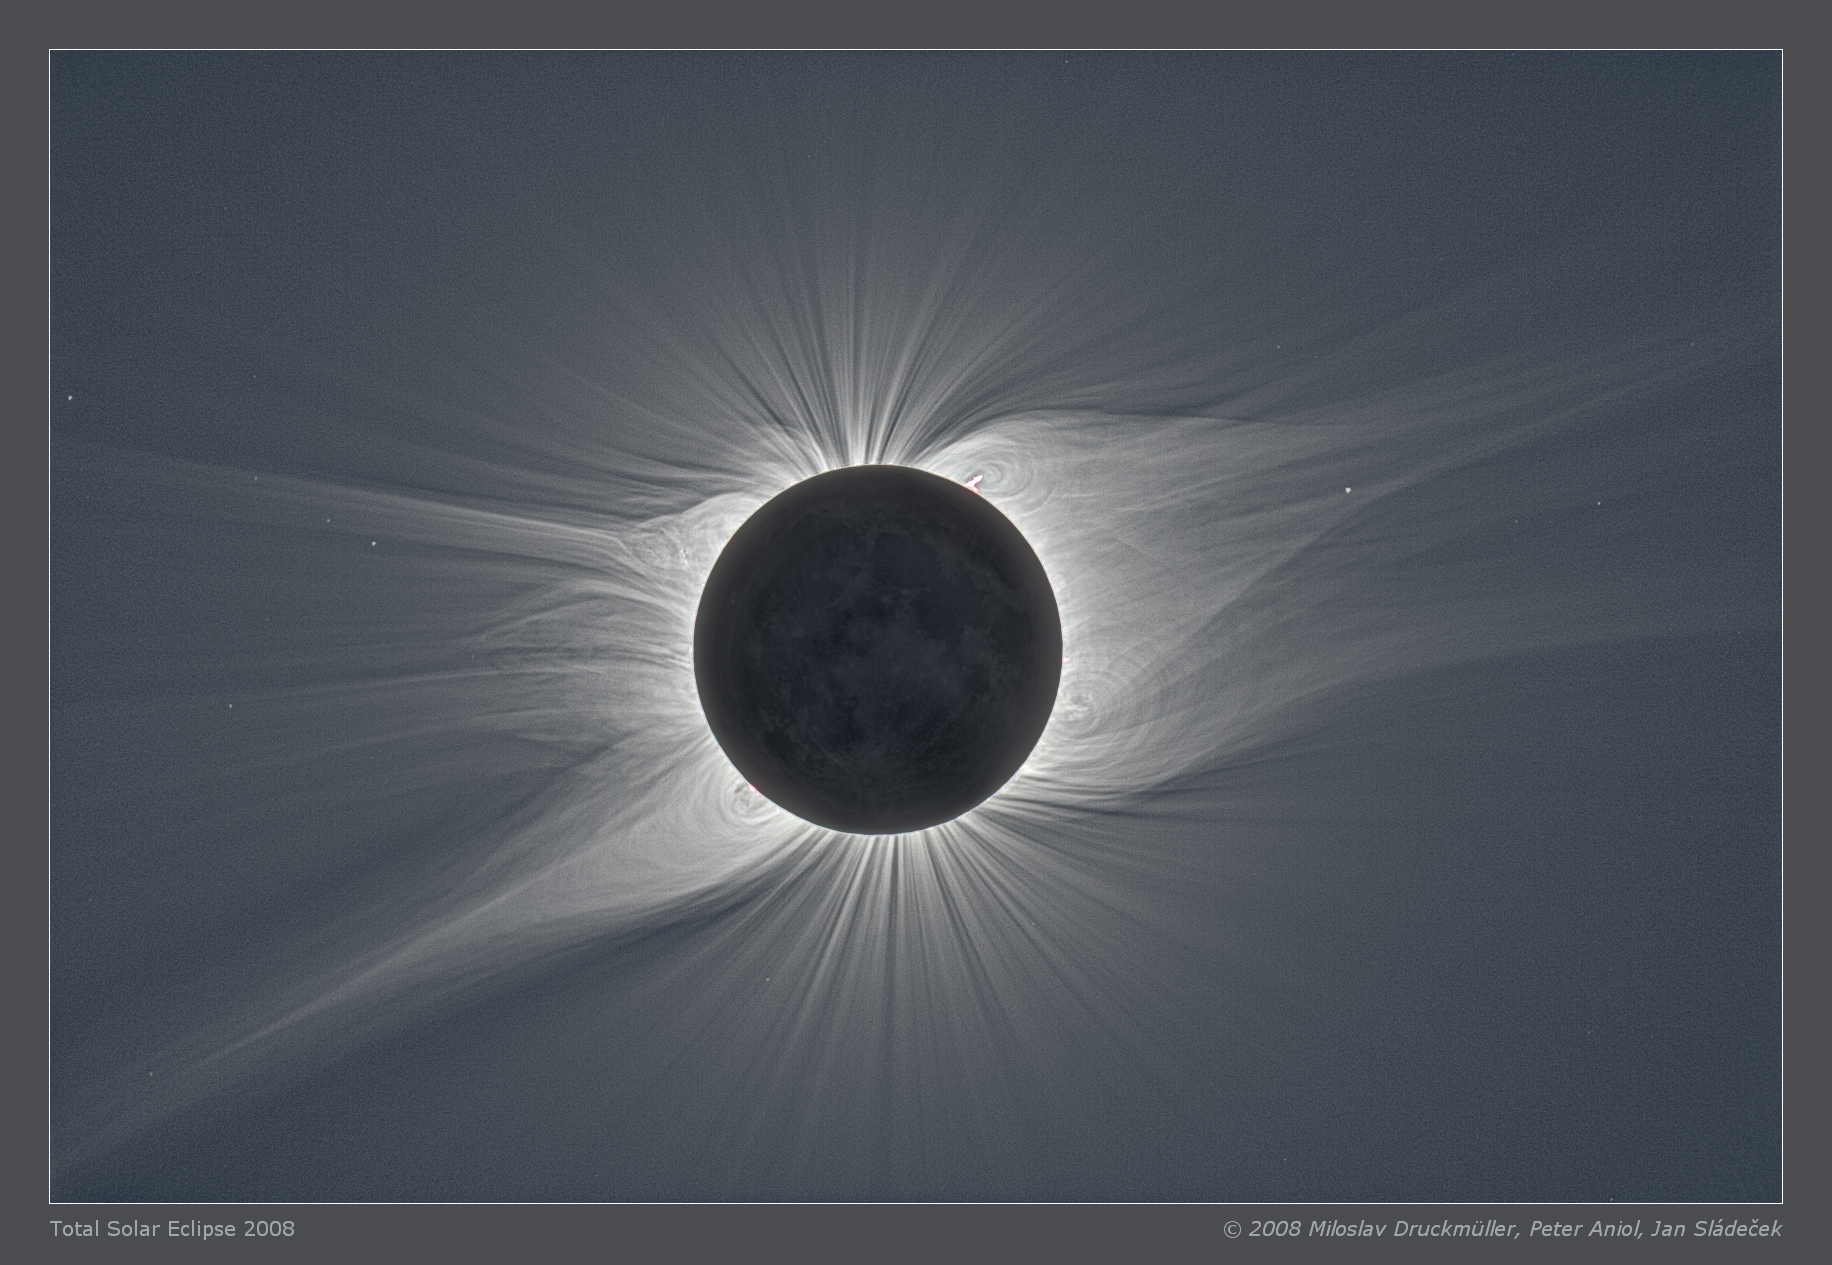
\includegraphics[width=0.6\textwidth]{images/Tse2008_500_mo1.png}
	}{
		\caption{Total solar eclipse image of the inner corona up to 5~solar radii. The picture was taken in Mongolia, 1~August~2008 and is processed from multiple images. Visible are the for a quiet Sun in cycle minimum typical magnetic field's dipole structure and the equatorial streamer belt. Credit: Miloslav Druckmüller, Peter Aniol, Jan Sládeček, 2008. get permission and preferred citation style... into acknowledgments? \url{http://www.zam.fme.vutbr.cz/~druck/Eclipse/}}
		\label{fig:Tse2008_500_mo1}
	}
\end{figure}
%figure source: http://www.zam.fme.vutbr.cz/~druck/Eclipse/Ecl2008m/Tse2008_500_mo1/Hr/Tse2008_500_mo1.png

%%% solar wind + heliosphere
Because of the high coronal temperatures, plasma escapes from the solar gravitational field \citep{Parker1958} with velocities of \SIrange{200}{800}{\km\per\s}. Its acceleration is linked to the coronal heating and its exact location and process remain an open question (cite?). At a distance of a few solar radii (?4--20) the magnetic field becomes too weak to guide the coronal plasma. From this source surface the solar wind flows radially outward into space until it reaches the termination shock, spanning the heliosphere. Eventually it collides with the local interstellar medium, creating the heliopause. The heliosphere is expected to be a bubble of teardrop shape (and may be led by a bow shock), caused by the Sun's relative velocity of \SI{23}{\km\per\s} to the local interstellar medium \citep{Owens2013}. Measurements of the Voyager~1 and 2 spacecraft indicate their passage of the termination shock at about \SI{94}{\au} and \SI{84}{\au}, entering the heliosheath region \citep{Owens2013}. \citet{Gurnett2013} report that in 2012 Voyager~1 actually crossed the heliopause into interstellar space at a solar distance of \SI{121}{\au}. \autoref{fig:Owens2013_Heliosphere_screenshot} illustrates the heliosphere and its surrounding flow structure.\\
\begin{figure}[htb]
	%\centering
	\fcapside[\FBwidth]{
		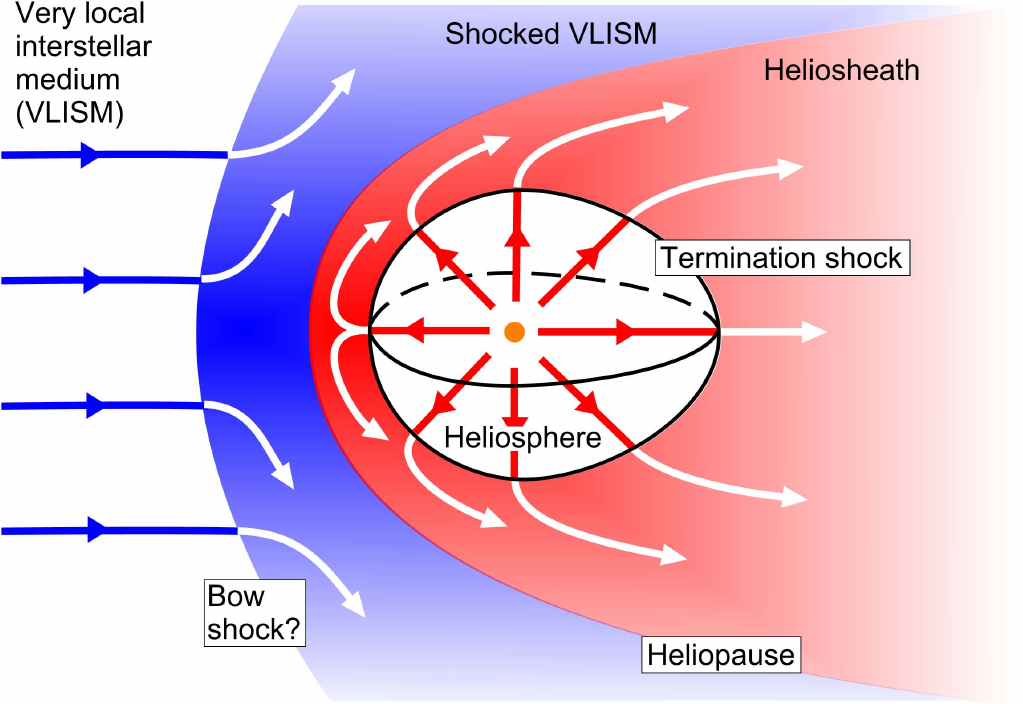
\includegraphics[width=0.6\textwidth]{images/Owens2013_Heliosphere_screenshot.png}
	}{
		\caption{Schema of the heliosphere and its surrounding flow structure. The heliosphere is formed by the interaction of the solar wind with the local interstellar medium at the heliopause. \citep[Fig.~9]{Owens2013} get permission...}
		\label{fig:Owens2013_Heliosphere_screenshot}
	}
\end{figure}

%%% solar wind influence + space weather
On its way outwards through the solar system the solar wind, carrying the solar magnetic field, interacts with the planets, their magnetic fields and other solar system bodies. These interactions have various effects, for instance disturbances in planetary magnetic fields with appearance of aurorae and enhanced radiation, atmospheric losses and stripping of cometary tails. Some of these effects can have disruptive consequences for humans and their technology. The topic of space weather effects is further addressed in \autoref{sec:space_weather}. The magnitude of these effects highly depend on spatial and temporal variations in the solar wind which are rooted in the dynamics of the solar magnetic field.\\

%%%%%%%%%%%%%%%%%%%%%%%%%%%%%
%\section{Stars/Beginning}
% introduction leading to stars; beginning from universe/big bang\\
% gravitational contraction of rotating nebula\\
% -> fusion burning; energy production\\
% In its core it fuses hydrogen to helium; 15.7~million~K; inner 25~\%\\
% energy transport -> radiation zone; up to 70~\%\\
% tachocline ~2~million~K\\
% energy transport by convection -> convection zone; up to surface\\
% convective granulation\\
% photoshere 4400--6600~K, effective black body temperature 5777~K; spectral class\\
% (herzsprung russell diagram)\\
% chromosphere... (solar atmosphere figure)\\
% transition region\\
%corona 1--3~million~K temperature (coronal heating problem)\\
% coronal holes: open magnetic field lines, solar wind\\
% heliosphere, shock with interstellar medium (ISM); Voyager\\

%%%%%%%%%%%%%%%%%%%%%%%%%%%%%
%big bang
%to formation of stars
%to ISM in our galaxy
%to formation of Sun
%Sun's inner structure (energy production and transport)
%its surface (radiation, spectral class)
%its outer structure (chromosphere, corona, solar wind, heliosphere)
%its heliosphere (termination shock with ISM, Voyager measurements)
%%%%%%%%%%%%%%%%%%%%%%%%%%%%%


\section{Solar dynamics}
\label{sec:solar_dynamics}

%%% differential rotation + solar magnetic field origin
The spin conservation of the contracting molecular cloud led to a rotation of the Sun with a current average period of about 25~days. The radial convective motion within the solar interior above the tachocline leads to a transport of momentum away from the rotation axis and therefore to a faster equatorial rotation in the convection zone \citep{Miesch2005}. This differential rotation is visible on the surface and was first discovered from sunspot observations. %in 1630 https://en.wikipedia.org/wiki/Solar_rotation
With a rotation period of about 34~days the poles have a lag of almost 9~days (for further information on solar rotation see appendix \autoref{sec:solar_rotation}). The differential rotation in the solar interior can be inferred from helioseismological observations, as seen in \autoref{fig:Miesch2005_fig1a_interior_diff_rot}. The resulting large rotational shear at the tachocline is believed to generate dynamo processes, creating the major part of the solar magnetic field \citep{Miesch2005}.\\
%Angular velocity profile in the solar interior inferred from helioseismology (after Thompson et al., 2003). In panel (a), a 2D (latitude-radius) rotational inversion is shown based on the subtractive optimally localized averaging (SOLA) technique. All inversions are based on data from the Michelson Doppler Imager (MDI) instrument aboard the SOHO spacecraft, averaged over 144 days. Inversions become unreliable close to the rotation axis, represented by white areas in panel (a). Note also that global modes are only sensitive to the rotation component which is symmetric about the equator (courtesy M.J. Thompson \& J. Christensen-Dalsgaard).

\begin{figure}[htb]
	\begin{floatrow}
		\ffigbox{	%[\FBwidth][]{
			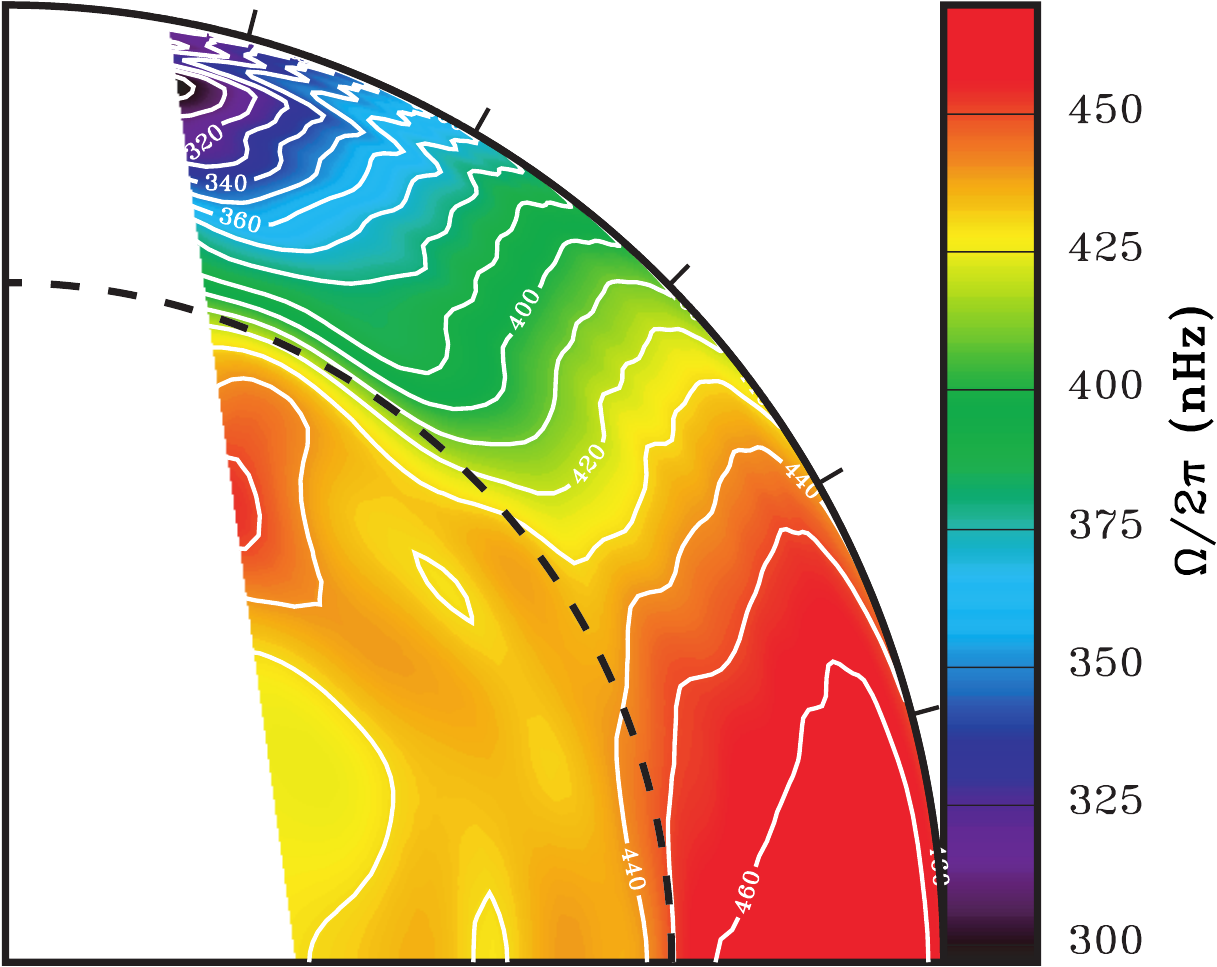
\includegraphics[width=0.5\textwidth]{images/Miesch2005_fig1a_interior_diff_rot.png}
		}{
			\caption{Angular rotation velocity in the solar interior. The radiation zone has a nearly solid rotation. Above the tachocline (dashed line) begins the differential rotation of the convection zone. The angular velocity is inferred from helioseismology via observations from the Michelson Doppler Imager (MDI) at the Solar and Heliospheric Observatory (SOHO) spacecraft. \citep[Fig.~3]{Thompson2003} get permission...}
			%(\citet[Fig.~1\,a]{Miesch2005}; based on \citet[Fig.~3]{Thompson2003})
			\label{fig:Miesch2005_fig1a_interior_diff_rot}
		}
		\ffigbox{
			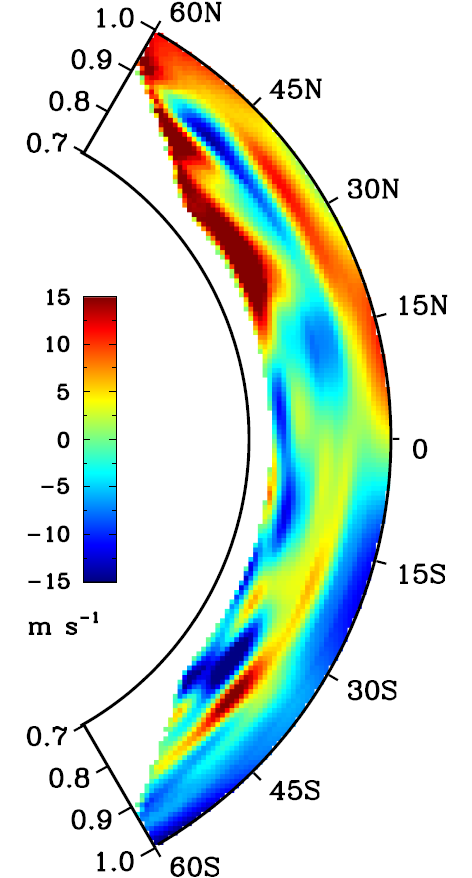
\includegraphics[width=0.28\textwidth]{images/Zhao2013_meridional_flow.png}
		}{
			\caption{Meridional flow velocity profile in part of the convection zone. Positive values are directed towards north. The velocity is inferred from helioseismology via observations from the Helioseismic Magnetic Imager (HMI) at the Solar Dynamics Observatory (SDO) spacecraft. \citep[Fig.~4\,a]{Zhao2013} get permission...}
			\label{fig:Zhao2013_meridional_flow}
		}
	\end{floatrow}
\end{figure}

%%% convection cycle + solar magnetic field + solar cycle
Helioseismic measurements reveal that the large-scale convective flow is agglomerated into large convection cells with slow meridional flows of a few \si{\m\per\s}. A poleward subsurface flow and equatorward backflow beneath is detected within each hemisphere, see \autoref{fig:Zhao2013_meridional_flow}. The cells have a convection cycle of about 22~years (cite...). As the magnetic field is carried by the plasma, it emerges at the surface with the same periodicity. Within one period the surface magnetic field configuration changes from a dipole structure to a reversed dipole structure with opposite polarity, thus the transition time from one dipole state to the next lasts about 11~years. In the transition phase magnetic flux emerges in belts above and below the solar equator, resulting in a multipolar structured magnetic field.\\

%%% sunspots
Since regions of strong magnetic flux are visible as sunspots on the photosphere, they were known well before the common era by chinese and greek scholars. %greek sunspot observation: http://adsabs.harvard.edu/abs/2007JBAA..117..346V
Systematic sunspot observations exist since 1610, shortly after the invention of the telescope (cite?). In 1843 Schwabe discovered the 11-year periodicity in the sunspot occurence (cite?). To record solar cycles in 1848 Wolf (et al?) introduced the sunspot number (SSN) and cycle number (with the zeroth occuring in 1749) (cite?), see \autoref{fig:ROB_ssn_wolfmms}.\\
\begin{figure}[htb]
	%\centering
	\fcapside[\FBwidth]{
		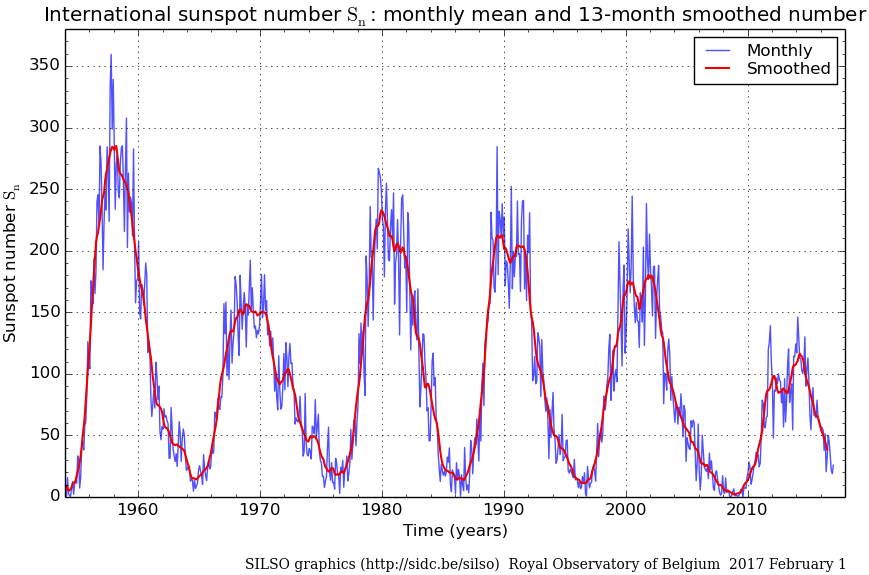
\includegraphics[width=0.6\textwidth]{images/ROB_ssn_wolfmms.png}
	}{
		\caption{The monthly mean sunspot number (blue) and 13-month smoothed monthly sunspot number (red) since 1954. Credit: SILSO data/image, Royal Observatory of Belgium, Brussels, \mbox{2017-02-01}. get permission... Update this figure before printing!!!}
		\label{fig:ROB_ssn_wolfmms}
	}
\end{figure}
%image from:	http://sidc.be/silso/
The large variations in cycle length ?(9--14~years) and intensity ?(0--350~Sn) make it difficult to predict the course of the next solar cycle (cite...).\\
lont-time variations like the Maunder minimum...\\

%butterfly
Observations of the surface radial magnetic field show the appearance of bipolar magnetic flux at belts of about \SI{+-20}{\degree} latitude at the beginning of a cycle and a shift to lower latitudes at the end of a cycle (magnetogram figure of sunspot?). Thus the plot of surface magnetic field over latitude and time reveals a butterfly pattern, see \autoref{fig:Hathaway_magbfly}. The emerging flux (its polarity alternates with each cycle) is carried by the slow meridional surface flow poleward, resulting in the polar field switch. The ordered dipole structure in solar cycle minimum leads to open polar field regions with coronal holes and a closed equatorial field belt.\\
\begin{figure}[htb]
	\centering
	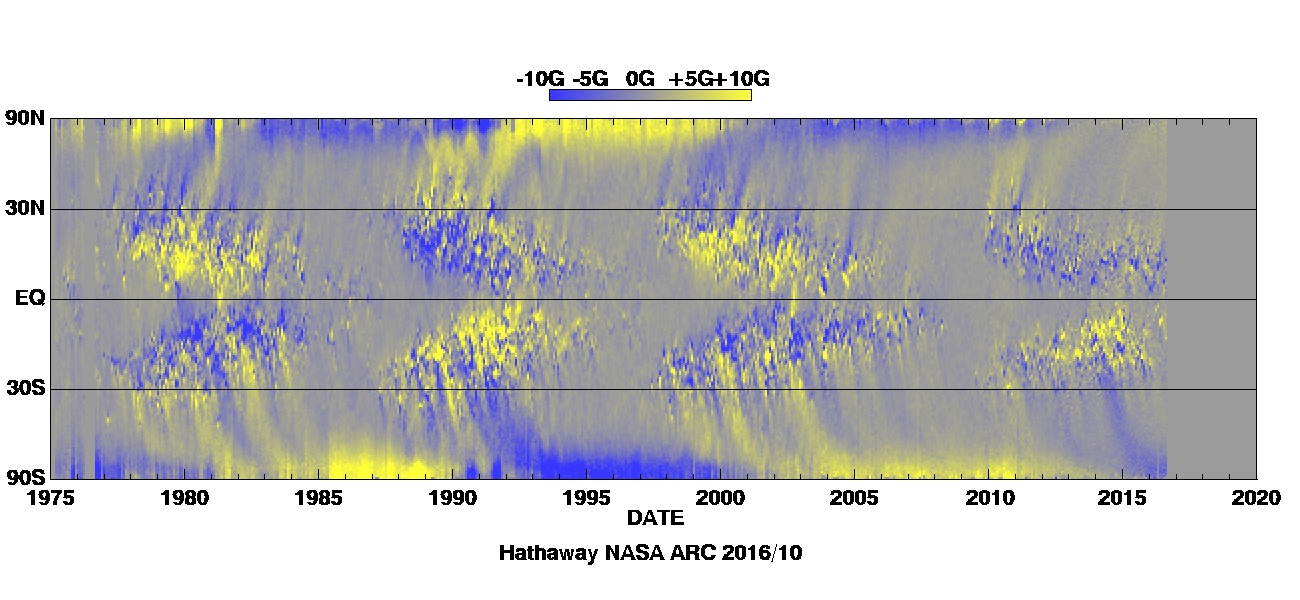
\includegraphics[width=\textwidth]{images/Hathaway_magbfly_201610.jpg}
	\caption{This magnetic butterfly diagram maps the synoptic radial magnetic field on the solar surface. Yellow represents an outward directed magnetic field (positive), blue inward (negative). The data is obtained from instruments on Kitt~Peak National Observatory and from the MDI at the SOHO spacecraft. Credit: David~Hathaway, NASA Marshall Space Flight Center; see also \citet[Fig.~17]{Hathaway2015}. Update this figure before printing!}
	\label{fig:Hathaway_magbfly}
\end{figure}
%figure source:	http://solarscience.msfc.nasa.gov/images/magbfly.jpg

compare with \autoref{fig:Tse2008_500_mo1}...\\

HMF geometry during maximum\\

fast solar wind emerges from CHs\\
\citet{Schwenn1983}: ``During the Skylab era in 1973/74 we learned that these high speed streams emerge from coronal holes (Hundhausen, 1977 and references therein).''\\

slow from closed field streamers\\

This is confirmed by the Ulysses spacecraft, which measured the solar wind speed in a polar orbit covering more than one solar cycle (\autoref{fig:McComas2008_Ulysses_orbit}).\\
\begin{figure}[htb]
	\centering
	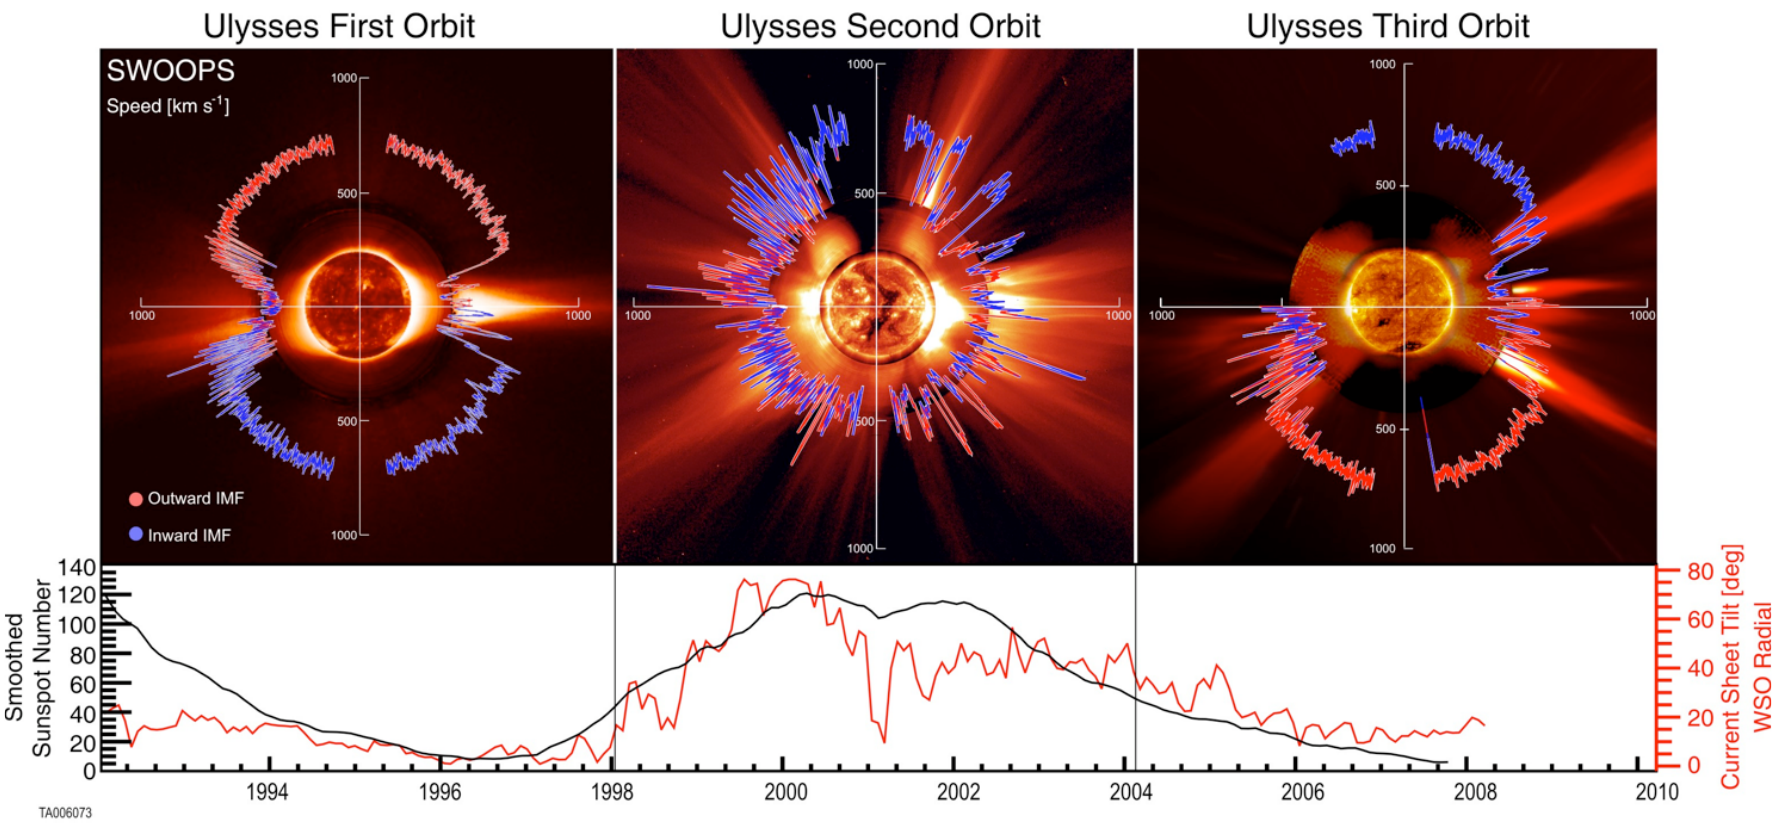
\includegraphics[width=\textwidth]{images/McComas2008_Ulysses_orbit_.png}
	\caption{Solar wind velocity and magnetic field polarity over latitude during low and high solar activity for the three orbits of the Ulysses spacecraft. The SSN and CS tilt angle are plotted as well. \citep[Fig.~1]{McComas2008}. ask for high res. image}
	\label{fig:McComas2008_Ulysses_orbit}
\end{figure}
%figure source: http://onlinelibrary.wiley.com/doi/10.1029/2003GL017136/full
%McComas2008: (a–c) Polar plots of the solar wind speed, colored by IMF polarity for Ulysses' three polar orbits colored to indicate measured magnetic polarity. In each, the earliest times are on the left (nine o'clock position) and progress around counterclockwise. (d) Contemporaneous values for the smoothed sunspot number (black) and heliospheric current sheet tilt (red), lined up to match Figures 1a–1c. In Figures 1a–1c, the solar wind speed is plotted over characteristic solar images for solar minimum for cycle 22 (8/17/96), solar maximum for cycle 23 (12/07/00), and solar minimum for cycle 23 (03/28/06). From the center out, we blend images from the Solar and Heliospheric Observatory (SOHO) Extreme ultraviolet Imaging Telescope (Fe XII at 1950 nm), the Mauna Loa K coronameter (700–950 nm), and the SOHO C2 white light coronagraph.

%++dynamics and magnetic field++\\
%rotating nebula to solar rotation\\
%rotation + convective motion -> differential rotation (first discovered by sunspot observations; helioseismology -> inner rotation, tachocline)\\
% meridional flow -> 22 year cycle || convective cells\\
% 22y convection cycle + magnetic field -> 11ys solar cycle (magnetic field activity cycle, polarity change, sunspot number)\\
SSN -> magnetic surface activity (butterfly diagram) => poloidal/toroidal field -> min/max polar CHs (quiet/active Sun figure) -> slow/fast sw pattern (Ulysses figure)) -> HMF (quiet B-field figure) -> Parker spiral (figure) -> solar wind\\

solar wind plasma composition and proberties -> visible solar wind structures (coronagraph image; with CME and streamer) -> stream interface (figure) -> in situ measurements (example in situ CIR/HSS plot)\\

stream interfaces (figure and link to previous CIR plot) -> HCS/HPS\\

CMEs (link to previous coronagraph image; in situ CME/MC plot; CME schema figure?)\\


switching between states of strong poloidal or toroidal field\\

differential rotation -> B-field\\
meridional flow -> solar cycle\\

dipole structure, open and closed field lines\\
polar coronal holes\\
streamer/equatorial streamer belt\\

solar wind\\

open field lines (coronal holes) -> HSSs\\
equatorial ballerina model -> CIRs (figure?)\\

%%% reconnections + CMEs
The solar differential rotation wraps the magnetic field lines, accumulating tension, leading eventually to relief with a magnetic reconfiguration by field line reconnections.\\
--> release of much energy --> flares, CMEs\\


solar wind's impact on Earth\\

the rotation axis is tilted from the normal of the ecliptic by $i_\odot = 7.25$\textdegree{} \citep{USNO2015} (refer to or put into appendix??).\\ %USNO2015 C3

%%%%%%%%%%%%%%%%%%%%%%%%%%%%%%%%%


\section{Solar wind}
\label{sec:solar_wind}

see Kivelson1995, p14+91\\
first observed at solar eclipses?, before? deduced by Parker from theory/Carrington from geomagnetic storms?\\

discovered via eclipses?\\
see eclipse photo from Druckmüller \autoref{fig:Tse2008_500_mo1}\\

in 1958 Parker predicted/postulated the solar wind \citep{Parker1958}\\
expanding isothermal atmosphere (solar wind model)\\
continuous supersonic radial outflow of plasma\\
-> also Parker spiral of HMF (see \autoref{fig:Owens2013_PFSS_Sectors_screenshot})


\section{Heliospheric magnetic field}	%better: interplanetary magnetic field??
%\label{sec:heliospheric_magnetic_field}

reviews: \citet{Balogh2009} (for heliosheath), \citet{Owens2013}\\

Winterhalter1994 The heliospheric plasma sheet:\\
"the narrow heliospheric current sheet (ca. 3000--10000 km thick), together with the heliospheric plasma sheet in which it is embedded. The heliospheric plasma sheet region is identified by a significantly enhanced plasma beta caused by density enhancements and diminished magnetic field strength and is about 20 to 30 times the thickness of the current sheet."\\
heliospheric current sheet (HCS)\\
heliospheric plasma sheet (HPS)\\
ballerina model... (search figure...)\\

%Cranmer2005:
%?insert their figure 1
Photosphere: magnetic bright points (MBP) 1--2~kG\\ %Cranmer2005
their convective motion result in wavelike fluctuations of the thin tubes\\
low chromosphere: thin flux tubes expand laterally and merge to a homogeneous network field\\
below the chromosphere-corona transition region: the network magnetic field expands laterally and merges again to a large-scale canopy (image)\\

[above the Alfv\'en critical point---where the wind speed equals the local Alfv\'en speed at about 10~$R_\odot$---both the inward and outward modes are advected (advect: convect horizontally) outward with the wind\\
superradially expanding magnetic flux tube\\
\citep{Cranmer2005}]\\
see also paper citations...\\

analytical solar magnetic field model for solar minimum conditions \citep{Banaszkiewicz1998}\\
dipole plus quadrupole plus current sheet (DQCS) solar magnetic field model\\
The DQCS model with its quadrupole part having a direct link from the solar equator to infinity along the equatorial plane and current sheet. (see \autoref{fig:Banaszkiewicz1998_DQCS_model_raw}) \citep{Banaszkiewicz1998}\\
compare with field geometry from eclipse \autoref{fig:Tse2008_500_mo1}...\\
\begin{figure}[htb]
	\begin{floatrow}
		\ffigbox{
			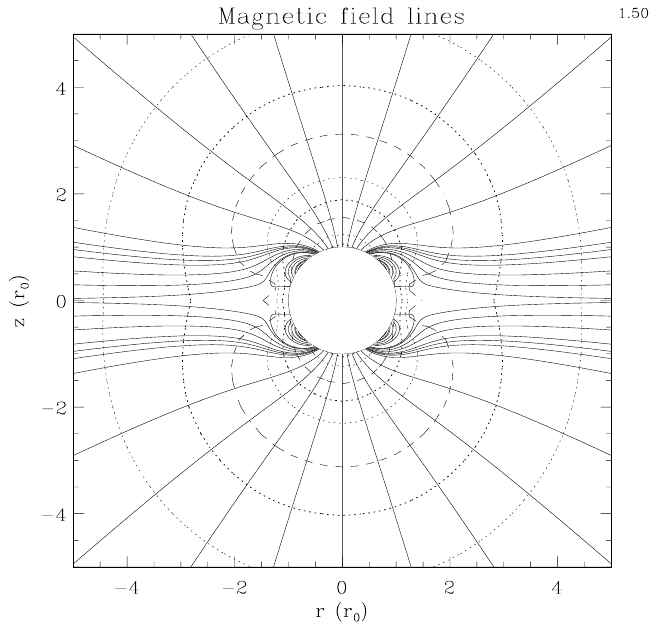
\includegraphics[width=0.45\textwidth]{images/Banaszkiewicz1998_DQCS_model_raw.png}
		}{
			\caption{Solar magnetic field geometry from the DQCS model with field lines (solid) and constant field strength surfaces (dashed). The quadrupole part allows equatorial outflows along the current sheet. \citep[Fig.~3]{Banaszkiewicz1998} get permission...}
			\label{fig:Banaszkiewicz1998_DQCS_model_raw}
		}
		\ffigbox{
			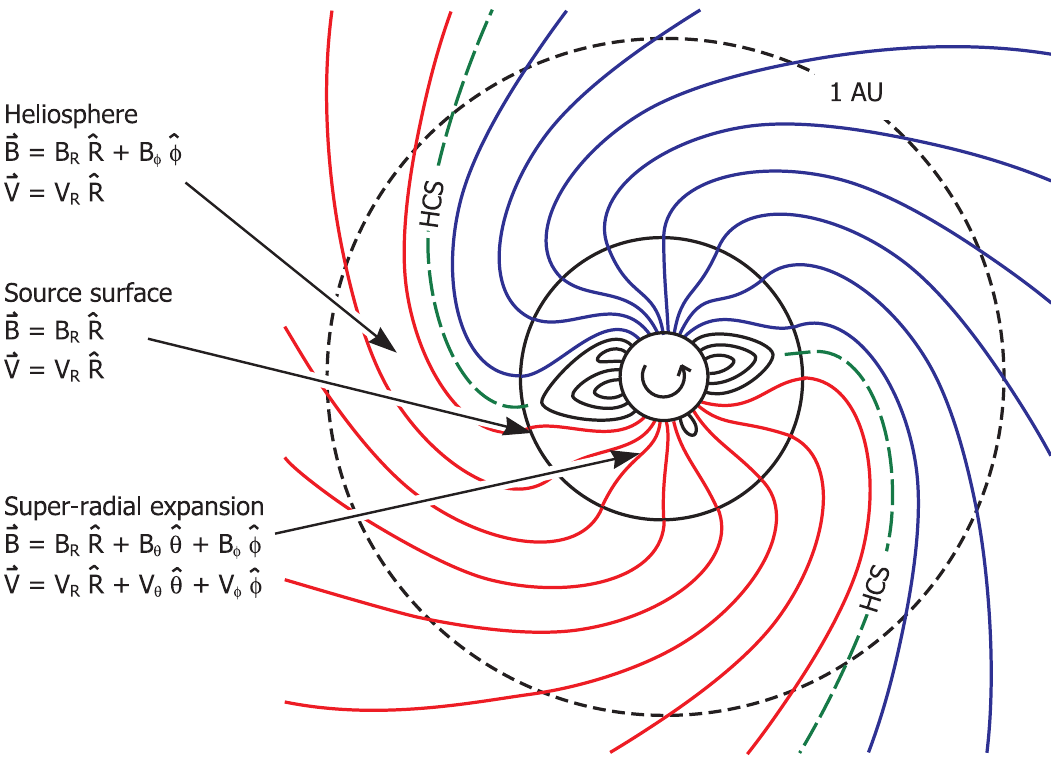
\includegraphics[width=\Xhsize]{images/Owens2013_PFSS_Sectors_screenshot.png}
		}{
			\caption{Illustration of the solar magnetic field Parker spiral formation by rotation of the solar wind source surface. Between solar wind flows of opposite magnetic field polarity a heliospheric current sheet (HCS) forms. (\citet[Fig.~1]{Owens2013}, adapted from \citet[Fig.~1]{Schatten1969}) get permission...}
			\label{fig:Owens2013_PFSS_Sectors_screenshot}
		}
	\end{floatrow}
\end{figure}

Parker spiral, source surface and HCS, see \autoref{fig:Owens2013_PFSS_Sectors_screenshot}\\
%A sketch of the steady-state solar magnetic field in the ecliptic plane. Close to the Sun, in a spatial region approximately bounding the solar corona, the magnetic field dominates the plasma flow and undergoes significant non-radial (or super-radial) expansion with height. At the source surface, typically taken to be a few solar radii, the pressure-driven expansion of the solar wind dominates and both the field and flow both become purely radial. In the heliosphere, rotation of the HMF footpoints within a radial solar wind flow generates an azimuthal component of the HMF, leading to a archimedean spiral geometry. Regions of opposite HMF polarity, shown as red and blue lines, are separated by the heliospheric current sheet (HCS), shown as the green dashed line. Image adapted from Schatten et al. (1969).

MHD simulations based on Voyager~1 and 2 measurements within the heliosheath indicate the formation of magnetic bubbles (reconnected sector regions) at the sector boundary caused by the compression before the heliopause, flowing away to the heliosheath tail \citep{Opher2011}.\\
%Opher2011: Is the Magnetic Field in the Heliosheath Laminar or a Turbulent Sea of Bubbles?


\section{Solar wind properties and structures}

list event/structure types\\
solar wind structures source regions: sunspots/active regions, coronal holes, filaments\\


\subsection{Solar wind plasma}
\label{sec:solar_wind_plasma}

Plasma in general (properties (H/He/metal composition; see paper...), Plasma-beta, etc.)\\
	solar wind properties, slow/fast wind, MHD waves (Alfv\'en waves)\\

special events/configurations, which can appear (CIRs, HCS/HPS, etc.)
HSS, sector boundaries, CIRs, CMEs\\


\subsection{Slow solar wind}

regions with closed lines\\
trapped plasma, slow solar wind from streamers\\


\subsection{High speed streams}

regions with open lines\\
coronal holes as sources of fast sw\\

sw plot of HSS with CIR to refer to\\


\subsection{Stream interaction regions}

Streams of fast wind catch slow wind\\
-> compressions, shocks, deflections\\

Corotating interaction regions (CIRs)\\
Stream interaction regions (SIRs)\\

formation of stream interface and stream deflection, see \autoref{fig:Owens2013_CIR_2panel_screenshot}\\
%A sketch of a stream interaction region. Left: Looking down on the ecliptic plane. Magnetic field lines within fast (slow) wind, shown in red (blue), become aligned with the stream interface by the reverse (forward) wave. Right: a view from Earth. The magnetic axis, M, and therefore the wind speed belts, are inclined to the rotation axis, R. The point in the heliosphere at which fast wind is able to catch up to the slow wind ahead of it is the stream interface (SI), which forms a spiral front in the heliosphere, shown as the black-outlined curved surface. In the frame of reference of the SI, both fast and slow wind flow toward the SI. Fast (slow) wind, shown by the red (blue) arrow, is slowed (accelerated) and deflected along the SI in the direction counter to (along) solar rotation. Right panel adapted from Pizzo (1991).
\begin{figure}[htb]
	%\centering
	\fcapside[\FBwidth]{
		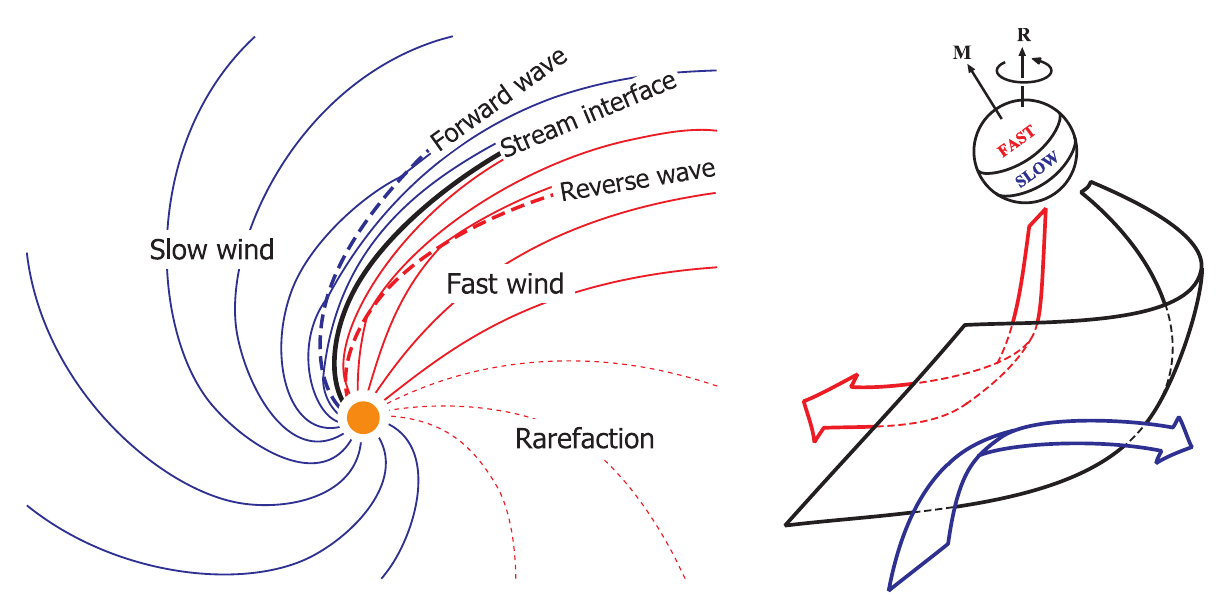
\includegraphics[width=0.6\textwidth]{images/Owens2013_CIR_2panel_screenshot.png}
	}{
		\caption{Schema of the formation of a stream interface (left) and deflection of streams (right), both generated from interactions between slow and fast solar wind. (\citet[Fig.~7]{Owens2013}; right panel adapted from \citet[Fig.~2]{Pizzo1991}) get permission...}
		\label{fig:Owens2013_CIR_2panel_screenshot}
	}
\end{figure}
refer to sw figure of CIR\\


\subsection{HCS / HPS}

from sector boundaries (ballerina skirt)\\


\subsection{Coronal mass ejections}
\label{sec:coronal_mass_ejections}

Coronal mass ejections (CMEs) (discovery (Carrington), definition (Hundthausen?), models, GCS (conception of 3-dim CME shape --> enables Earth arrival time forecast from modeled direction and velocity))\\

active regions:\\
sunspots, magnetic reconnections, flares, post-eruptive arcades\\

coronagraph figure of CME (COR2 image, SECCHI/STEREO)\\
in situ solar wind figure of same CME (recent one from 2016)\\

CME-plasma properties\\


\subsubsection{Magnetic clouds}
%\label{sec:magnetic_clouds}

magnetic cloud (MC); refer to in situ plot\\
See BS magnetic cloud model in analyses methods chapter
MVA...\\


\section{Space weather}
\label{sec:space_weather}

Solar wind influences the Earth's magnetosphere and can disturb sensitive technical systems\\
understanding its properties helps with prediction of events\\

influences on human infrastructure/technical systems\\

various space weather effects, for instance disturbances in magnetic fields, aurorae, episodes of enhanced radiation, atmospheric losses and stripping of cometary tails. figures of these effects?\\


\subsection{Solar influence on Earth}
\label{sec:solar_influence_on_earth}

Carrington made first connection between terrestrial magnetic field and solar flares. correct?\\

%see Bartels1962:
there are several types of solar-terrestrial relations, \citet{Bartels1962} listed:\\	%Zuordnung solarer Beobachtungen zu terrestrischen\\
a) irregular flare and CME effects (Carrington)\\
b) 11"~year solar cycle effects\\
c) 27"~day solar rotation effects\\
d) daily effects (x-ray and light)\\

seasonal effects from Earth orbital distance, inclination (solar rotation axis angle) and Earth tilt (get figure...)\\

solar wind and its species\\
solar radiation\\
solar energetic particles (SEPs)\\
gravitation\\

magnetosphere\\
ionosphere?\\
aurorae\\
geomagnetic storms (several days, from CMEs)\\
substorms (few hours, from CIRs??)\\

for humans and their technology important effects: enhanced radiation, geomagnetic storms\\
lovely, disruptive, dangerous consequences\\

at Earth the solar wind total energy flux ($1.45~\text{mW/m}^2$) is only about one millionth of the solar radiation flux (see \citet[p.~153]{Schwenn1990})\\


\subsection{Magnetosphere}
\label{sec:magnetosphere}

shape formed by dynamic pressure..., similar to heliosphere in ISM...\\

bow shock, magnetotail, magnetosheath, magnetopause\\
add ecliptic and terrestrial tilt angle; with plasmoid?\\
see \autoref{fig:heliosphere_image002}\\
\begin{figure}[htb]
	%\centering
	\fcapside[\FBwidth]{
		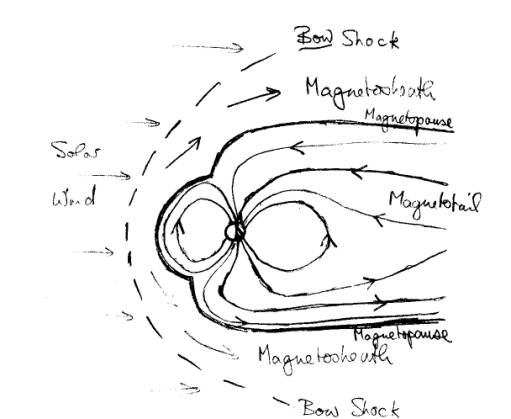
\includegraphics[width=0.5\textwidth]{images/heliosphere_image002.jpg}
	}{
		\caption{temp figure ``The cavity is called the magnetosphere. It has a relatively well-defined outer boundary, the magnetopause.''}
		\label{fig:heliosphere_image002}
	}
\end{figure}

turbulence with sw (KH or RT instabilities), see \autoref{sec:solar_wind_magnetosphere_coupling}\\

Earth magnetic field strength at a height of 36\,000~km (geostationary): ~100~nT\\
Earth magnetic field strength at the surface - equator: ~30\,000~nT - poles: ~60\,000~nT (cite?)\\

magnetopause = current layer??\\

two extreme cases of Bz orientation: parallel/antiparallel\\
compression/reconnection (with figure)\\

standoff distance:	\citep[p.~112]{Bothmer2007}
\begin{align}
	d = \frac{107.4}{1 R_\text{E}} (N V^2)^{-1/6}
\end{align}

Even in ``ancient'' times (when?) a correlation between solar particles and disturbances in the magnetosphere were known of (Bartels1962).\\

magnetosphere variations due to solar wind\\
magnetosphere protects from radiation (maybe from solar wind stripping atmosphere away?)\\

effects: aurorae, ...\\

ring current systems\\

definition of:\\
magnetic storm...\\
substorm...\\

subsection Ionosphere?\\
its variations due to solar radiation (day/night cycle and flares)\\
ionosphere -> TEC -> GNSS error\\


\subsection{Geomagnetic indices}
\label{sec:geomagnetic_indices}

%%% various indices
for Kp, AA and Dst read Section 7.4 in book \citet{Bothmer2007}...\\
Geomagnetic indices (variety of indices AA, AE, Dst, etc.)\\
Kp index, construction from 13 K stations... (-> look into early presentations)\\	%see GFZ Potsdam website
% http://isgi.unistra.fr/indices_kp.php (nice figure with Kp obs locations)
The Kp index is described in \autoref{sec:kp_index}.\\

AE - intensity of northern polar electrojet\\
Dst - intensity of magnetospheric ring current\\
Ring-Current Index Dst (read book Jursa1985 p. 4-31)\\


\subsection{Solar wind--magnetosphere coupling}
\label{sec:solar_wind_magnetosphere_coupling}

E"~field:	%VBth p124
\begin{align}
	\textbf{E}_\text{IMF?} = -\textbf{V} \times \textbf{B}_\text{IMF}
\end{align}
...derive from Lorentz force\\
(Because of high plasma conductivity the E"~field is not existent.)\\

Axford1964 viscous interaction (of turbulent nature, KH/RT instabilities, KH instabilities at the flanks of the magnetosphere) is a viable source of drag force/solar storm energy input into magnetosphere\\

Otto\&Nykyri1982 KH instabilities/vortices force magnetic reconnection even at northern IMF and are able to account for observed mass flux\\

\citet{Newell2007} and \citet{Newell2008}: coupling consists of merging and viscous part (reconnection and turbulence)\\
merging part: rate magnetic flux is opened at the magnetopause\\
viscous part: reconnection due to Kelvin-Helmholtz instabilies at the boundary\\

Merkin2013 MHD simulation of velocity shear at magnetosphere boundary with northern IMF; KH instabilities; double-vortex sheet structure\\


\chapter{Data}
\label{chap:data}

%COFI -- chapter outline and flow integration\\


\section{Instruments}
%\label{sec:instruments}

For analyzing the Sun and solar wind there are remote instruments (solar imager and coronagraphs) and in situ instruments (magnetometer and plasma detector).\\
Here the basic principles of latter are described, as we only use them...\\

several spectrometers with different energy ranges\\

isotope spectrometer - isotopic abundances of SEPs\\
ionic charge analyzer - charge state of SEPs\\
sw ion mass spectrometer - \\
sw ion composition spectrometer - \\
radio burst tracker\\


\subsection{Magnetometer}
%\label{sec:magnetometer}

Spacecraft nowadays carry two different magnetometer types, one for measuring the magnetic field direction and its strength and the other for observing the magnetic flux and detecting waves.\\

flux gate magnetometer -- two coils around core, one coil with alternating current, wich is compared with the induced current signal from the other; without external magnetic field both patterns match. the core is easier magnetized in direction of an existing external magnetic field -> patterns differ\\
search coil magnetometer -- a coil around a core; measures plasma waves\\

Because these magnetometer types are directional, they often are placed in two sets of triaxial configurations, attached on booms to decrease the influence of the spacecraft's own magnetic field.\\
L-> which is generated by surface charges?/electrons?/ionization?/the instruments?\\
%https://en.wikipedia.org/wiki/Spacecraft_magnetometer


\subsection{Plasma detector}
%\label{sec:plasma_detector}

A plasma detector measures the ion energy frequency distribution, which consists basically only of protons and alphas in solar wind (see \autoref{fig:ion_energy_spectrum_plot}). see also \autoref{sec:solar_wind_plasma}
\\
\begin{figure}[htb]
	%\centering
	\fcapside[\FBwidth]{
		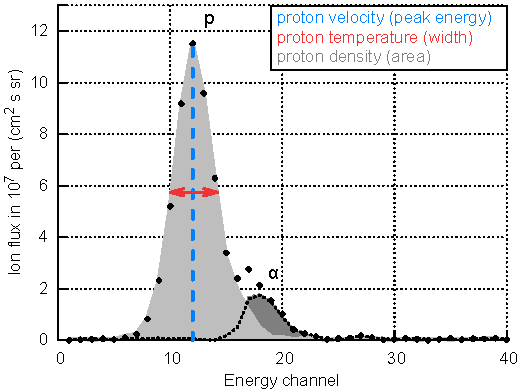
\includegraphics[width=0.5\textwidth]{images/gnuplots/ion_energy_spectrum_plot.pdf}
	}{
		\caption{Example of an ion energy spectrum with synthetic data. Here proton and helium (alpha) peaks are distinguishable...}
		\label{fig:ion_energy_spectrum_plot}
	}
\end{figure}
%figure adapted from source: http://www.goembel.biz/sun.html

From the energy spectrum the velocity, density and temperature an be derived.\\


average energy --> bulk velocity\\
distribution area --> number density\\
distribution width --> temperature\\

% source: ftp://spdf.gsfc.nasa.gov/pub/data/ulysses/plasma/swoops/ion/swoops_ion_users_guide_update_20030214.txt
% ``Plasma parameters are calculated by numerical integration of velocity-weighted
% ion distributions over an E/q range chosen to include the thermal proton and
% alpha-particle populations. Under extremely hot conditions, there can
% sometimes be some overlap between these populations. Additionally, during
% periods when the solar wind temperature is exceptionally low the experiment can
% not properly measure the temperature. Care has been taken to estimate the
% instrument background from channels that do not contain data, and the effects
% of background have been removed from the integration. The velocity space 
% resolution of the experiment is better in the energy dimension than in the
% angular dimensions.''


\section{Data sources}
%\label{sec:}

Spacecraft / data sets\\

Positions:\\
Earth:\\
	imager, magnetosphere\\
L1 - Lagrangian point:\\
	ACE (siehe auch space weather spacecraft Liste)\\
	Wind etc. (OMNI)\\
inner heliosphere:\\
	Helios~1 \& 2\\
outer heliosphere:\\
	Voyager~1 and 2\\
	Ulysses\\

also RT-data sources?\\


\subsection{Sunspot number}
%\label{sec:sunspot_number}

SSN history\\
add SSN figure of history incl. Maunder minimum?\\

SIDC/SILSO...\\
WDC-SILSO -- World Data Center-Sunspot Index and Long-term Solar Observations\\
%https://de.wikipedia.org/wiki/Sonnenfleck#Geschichte


\subsection{Kp index}
\label{sec:kp_index}

Kp index first introduced by \citet{Bartels1949}\\
it was maintained at the University of Göttingen...\\

insert figure of Kp musical diagram\\

mention IAGA...\\

The German Research Centre for Geosciences (GFZ) in Potsdam supplies indices of global geomagnetic activity, more precisely the Kp index and thereof derived indices. The GFZ provides historical and quicklook data of the indices via their website\footnote{GFZ website: \url{http://www.gfz-potsdam.de/sektion/erdmagnetfeld/daten-produkte-dienste/kp-index/} (existent in 2017-02-12)}.\\
list Kp derived indices\\
ap, Ap, K, Cp, ...\\


\subsection{OMNI data set}
\label{sec:omni_data_set}

a data set merged from different sources\\
The OMNI data \citep{King2005} were obtained from the GSFC/SPDF OMNIWeb interface.\\

from spacecraft located near the Lagrange point L1 upstream of Earth\\
time-shifted to the bow shock of the magnetosphere\\

OMNI2 H0 MRG1HR (1963-201308)
Cite from CDAweb: Hourly near-Earth solar wind magnetic field and plasma data, energetic proton fluxes (>~1 to >~60~MeV), and geomagnetic and solar activity indices.

NASA, Goddard Space Flight Center (GSFC), Space Physics Data Facility (SPDF): \url{http://spdf.gsfc.nasa.gov/}\\	%exintent in 2016-08-18
- Coordinated Data Analysis Web (CDAWeb): \url{http://cdaweb.gsfc.nasa.gov/}\\	%exintent in 2016-08-18
- OMNIWeb Plus: \url{http://omniweb.gsfc.nasa.gov/}\\	%exintent in 2016-08-18
%OMNIWeb Data Documentation: http://omniweb.gsfc.nasa.gov/html/ow_data.html


OMNI spacecraft data coverage (see also talk 2014-02-18)\\
see \autoref{fig:omni_data_coverage_1963-2013_plot}
\begin{figure}[htb]
	%\centering
	\fcapside[\FBwidth]{
		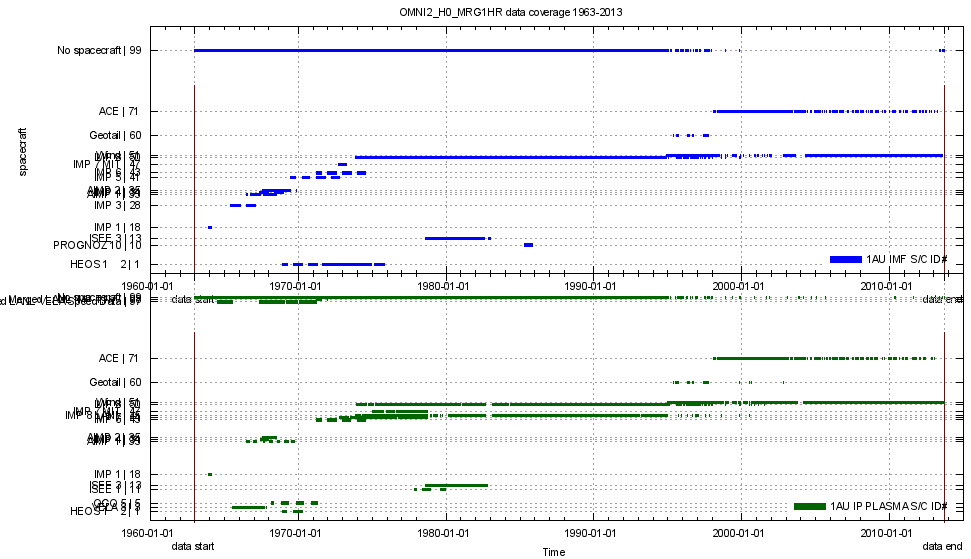
\includegraphics[width=0.5\textwidth]{images/gnuplots/omni_data_coverage_1963-2013_plot.png}
		\caption{OMNI intercalibrated multi-spacecraft data coverage per spacecraft. renew plot until 2016-11; integrate into 1 panel...}
	}{
		\label{fig:omni_data_coverage_1963-2013_plot}
	}
\end{figure}


\subsubsection{Advanced Composition Explorer}

s/c figure, launch date was 25 August 1997\\

MAG -- fluxgate magnetometer\\
SWEPAM\\	%https://sci-hub.ac/10.1023/A:1005040232597

data errors/gaps...\\

DSCOVR as replacement..., launched on 11 February 2015, NOAA's SWPC real-time solar wind prime source since 27 July 2016\\
\url{http://www.swpc.noaa.gov/products/real-time-solar-wind}\\


\subsubsection{Solar Wind Structures}

Solar Wind Structures (SWS) list\\
derived by Richardson.... from OMNI data (only?)

permission received.\\

%http://cedarweb.vsp.ucar.edu/wiki/index.php/Tools_and_Models:Solar_Wind_Structures
characterization of near-Earth solar wind structures since 1963\\
SWS lists \citep{Richardson2000} and \citep{Richardson2012}


\subsection{Helios probes}
\label{sec:helios_probes}

see Helios data readme.txt\\

two different fluxgate magnetometers and a search coil magnetometer\\

see \autoref{fig:MPS_Helios}
\begin{figure}[htb]
	\begin{floatrow}
		\ffigbox[\FBwidth][]{
			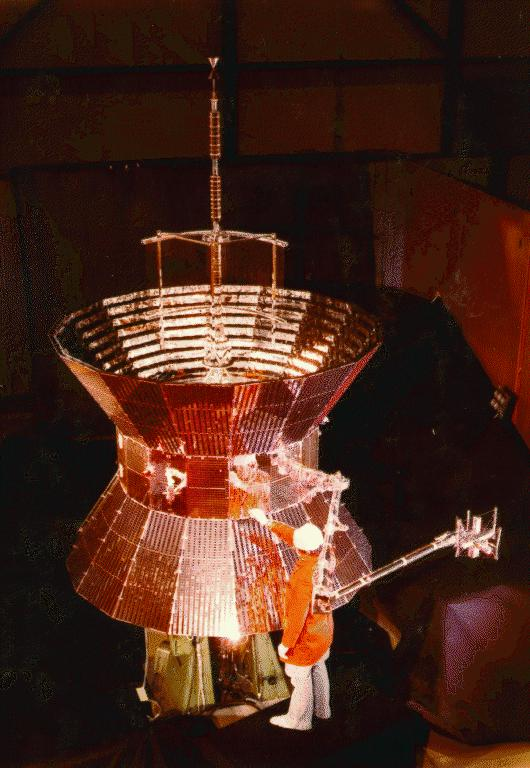
\includegraphics[width=0.3\textwidth]{images/MPS_Helios.jpg}
		}{
			\caption{One of the nearly identical twin Helios spacecraft. Credit: Max Planck Institute for Solar System Research. get permission...}
			\label{fig:MPS_Helios}
		}
		\ffigbox[\Xhsize]{
			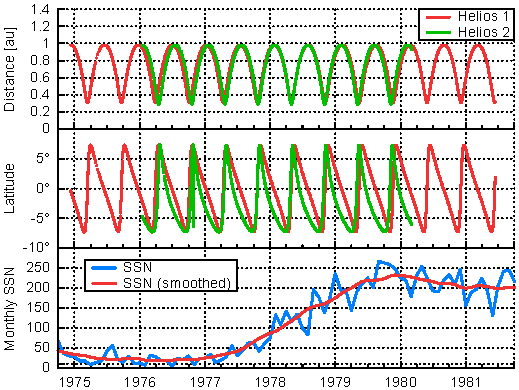
\includegraphics{images/gnuplots/Helios12_1h_r_b_ssn_plot.pdf}
		}{
			\caption{Plot of the Helios probes' solar distance and HGI latitude over their mission time, together with the monthly SSN and 13-month smoothed monthly SSN.}
			\label{fig:Helios12_1h_r_b_ssn_plot}
		}
	\end{floatrow}
\end{figure}

solar distance, HGI latitude and sunspot number during the Helios missions; see \autoref{fig:Helios12_1h_r_b_ssn_plot}\\

Helios orbit in the ecliptic plane (see \autoref{fig:Helios12_1h_magswe_ecliptic_plot}) and in the latitude polar plane (see \autoref{fig:Helios12_1h_magswe_polar_plot}); make 2-panel figure...\\
\begin{figure}[htb]
	\begin{floatrow}
		\ffigbox{
			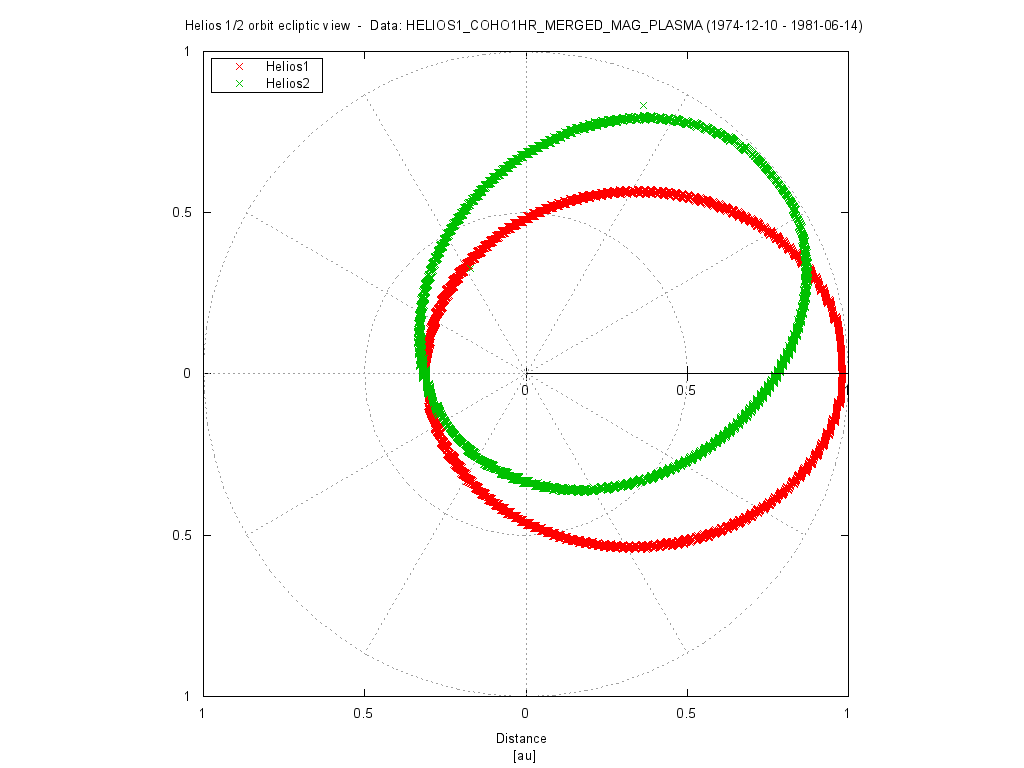
\includegraphics[width=0.45\textwidth]{images/gnuplots/Helios12_1h_magswe_ecliptic_plot.png}
		}{
			\caption{Plot of the Helios orbits in the ecliptic plane (left) and polar plane (right) (in HGI-coordinates). combine with polar plane plot...}
			\label{fig:Helios12_1h_magswe_ecliptic_plot}
		}
		\ffigbox{
			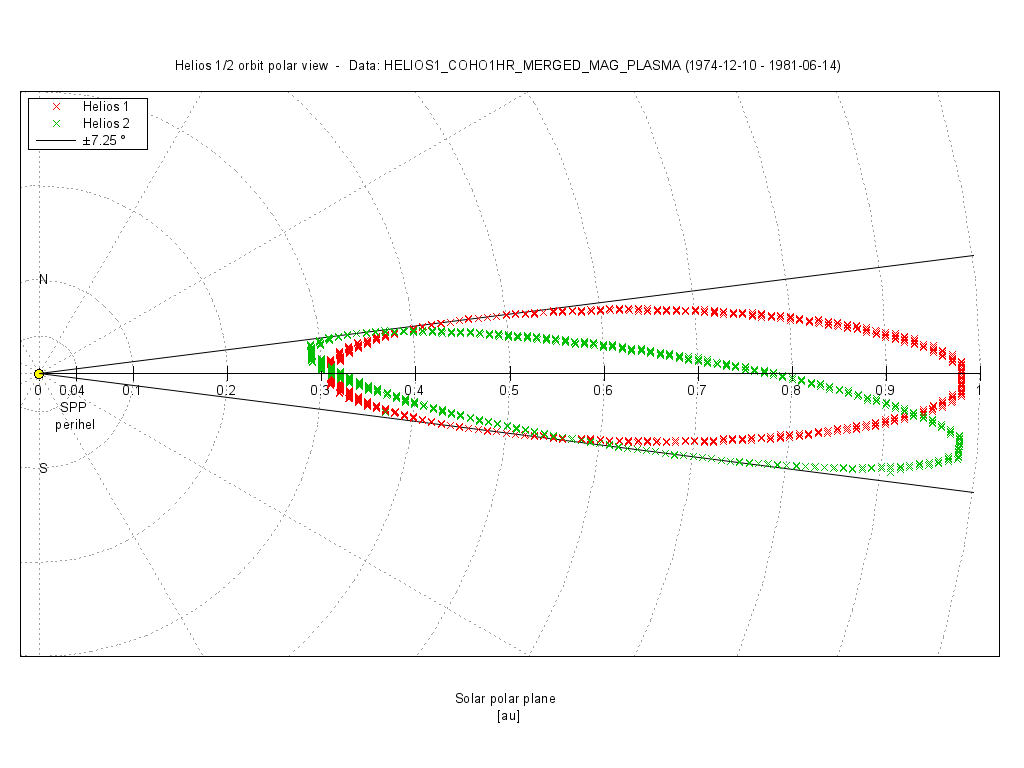
\includegraphics[width=\Xhsize]{images/gnuplots/Helios12_1h_magswe_polar_plot.png}
		}{
			\caption{combine with other plot...}
			\label{fig:Helios12_1h_magswe_polar_plot}
		}
	\end{floatrow}
\end{figure}

The Helios magnetic field and plasma data counts over solar distance are plotted in \autoref{fig:Helios12_1h_magswe_r-count_plot} and over latitude are plotted in \autoref{fig:latitude_frequency_plot}. build 2-panel figure...\\
\begin{figure}[htb]
	\begin{floatrow}
		\ffigbox{
			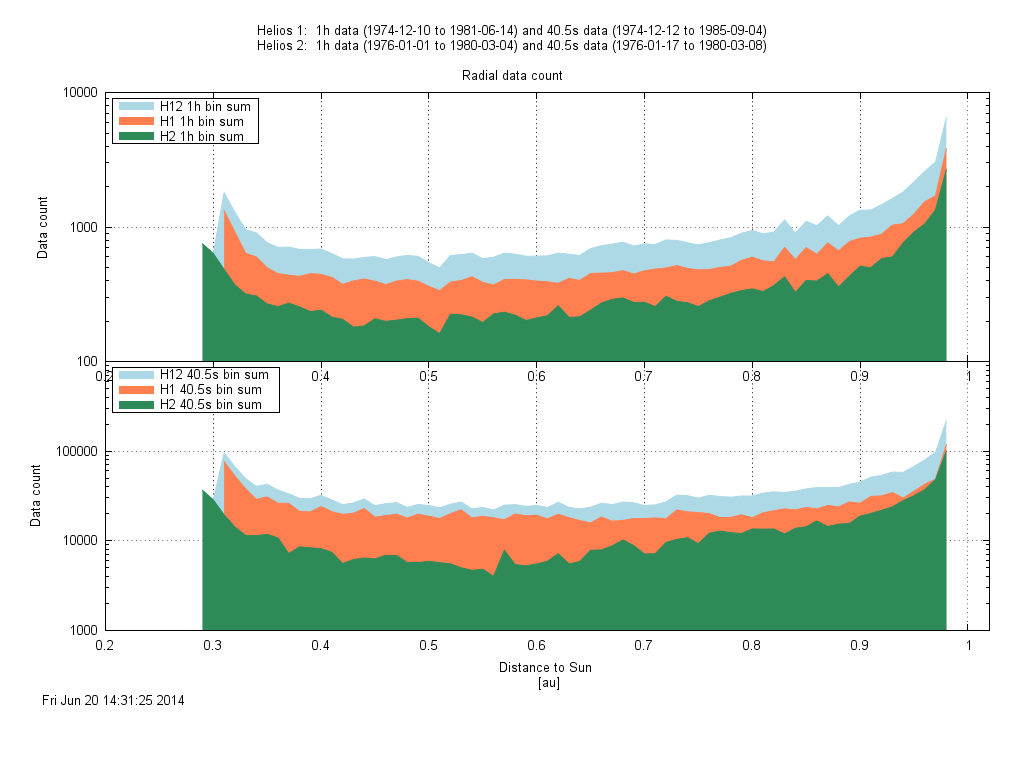
\includegraphics[width=0.45\textwidth]{images/gnuplots/Helios12_1h_magswe_r-count_plot.png}
		}{
			\caption{Plot of the Helios data count per 0.01~au solar distance bins. plot for mag and plasma individually..., combine with latitude plot...}
			\label{fig:Helios12_1h_magswe_r-count_plot}
		}
		\ffigbox{
			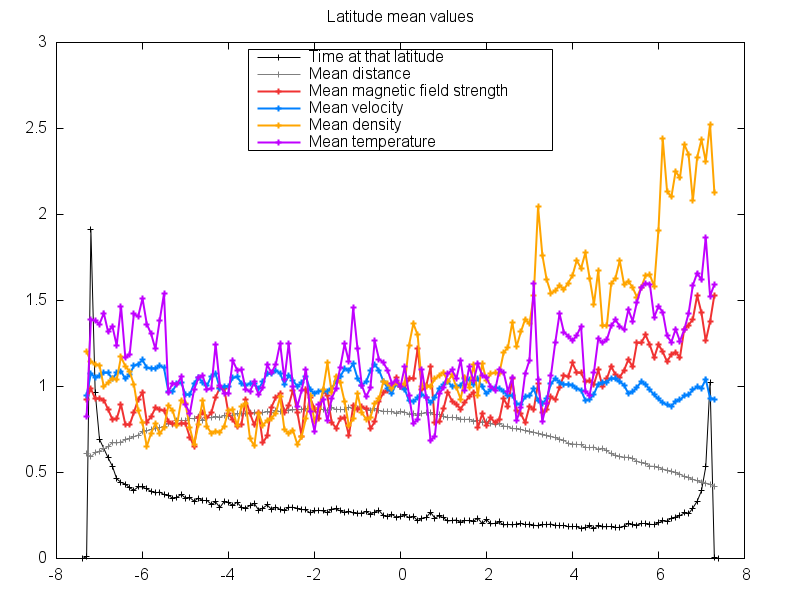
\includegraphics[width=\Xhsize]{images/gnuplots/latitude_frequency_plot.png}
		}{
			\caption{Plot of the Helios data count per 0.1° latitude. plot for mag and plasma individually... remove all other curves...}
			\label{fig:latitude_frequency_plot}
		}
	\end{floatrow}
\end{figure}

Solar wind data courtesy of R.~Schwenn, Max-Planck-Institut für Aeronomie, Lindau, magnetic field data courtesy of F.~Neubauer, Universität zu Köln. (see paper; into acknowledgements...)\\

%see presi 1.07 Inside Helios-Origins and Evolution-Salem.ppt
%see book Schwenn1990 https://books.google.de/books?id=W1DuCAAAQBAJ&printsec=frontcover&dq=Physics+of+the+Inner+Heliosphere+I.+Large-Scale+Phenomena&hl=de&sa=X&redir_esc=y#v=onepage&q=Physics%20of%20the%20Inner%20Heliosphere%20I.%20Large-Scale%20Phenomena&f=false



data sources -- see paper for replacing the following data\\
solar wind parameters: ACE, Helios, OMNI\\
geomagnetic indices: Kp, OMNI\\

Space Physics Data Facility (SPDF)\\

HELIOS 1 and 2 - orbital Parameters\\
\url{http://spdf.sci.gsfc.nasa.gov/pub/data/helios/helios1/traj/}\\
\url{http://spdf.sci.gsfc.nasa.gov/pub/data/helios/helios2/traj/}\\

Helios hourly merged mag \& plasma data:\\
HELIOS1\_COHO1HR\_MERGED\_MAG\_PLASMA\_2965.txt\\
HELIOS2\_COHO1HR\_MERGED\_MAG\_PLASMA\_3096.txt\\
\url{http://cdaweb.gsfc.nasa.gov}\\
temporal coverage of merged data\\
Helios 1: 1974-12-10 - 1981-06-14\\
Mag data availability: 42.6~\%\\
Plasma \& orbit data availability: 76.4~\%\\
Helios 2: 1976-01-01 - 1980-03-04\\
Mag data availability: 54.4~\%\\
Plasma \& orbit data availability: 91.8~\%\\

		%introduction and basics
	\chapter{Data}
\label{chap:data}


	%####--  Chapter2  --####
	
\chapter{Solar wind and CME influence on the magnetosphere}
\label{chap:chapter2}

Impact estimations derived from empirical correlations between in-situ solar wind measurements and the geomagnetic \Kp{}~index\\

%context
Variations in the Earth's magnetosphere are largely evoked by influence through the solar wind. These magnetospheric disturbances have diverse effects on the terrestrial environment. Especially the effects of severe geomagnetic storms created by coronal mass ejections (CMEs) pose various threats to sensitive technical systems and exposed humans. Thus, the development of quantitative forecasts for magnetospheric impacts caused by solar wind and CMEs is of major importance. The analyses in this chapter are based on my work done for the EU~FP7 project Advanced Forecast For Ensuring Communications Through Space (AFFECTS).

%aims
The goals of this study are to estimate the magnetospheric impact from solar wind and also to predict it for remotely forecasted CMEs and streams in particular. Empirical dependencies between the solar wind and the magnetospheric disturbance index~\Kp{} are presented. These relations allow nowcasts from upstream (L1) solar wind in-situ measurements and allow forecasts from remote observations of the corona. The \Kp{} nowcast is derived via a relation with the solar wind electric field. The \Kp{} forecasts are based on solar wind velocity and split into CME and stream forecasts. The magnetospheric impact of CMEs is estimated solely based on their arrival velocities that may be predicted from coronagraph observations. The prediction of solar wind stream velocities, e.g., obtained from coronal hole observations, enables to estimate their impact as well.

% data
The solar wind data considered in these analyses consists of 35~years (1981--2016) of high-resolution minutely OMNI data, which is composed of multi-spacecraft intercalibrated in-situ measurements from \SI{1}{\au}. I analyze the \Kp{} frequency distributions with respect to the depending parameters E"~field and velocity, derive their mean \Kp{} values and further compile functional dependencies via logarithmic fitting.

%methods
In order to nowcast the \Kp~index from general solar wind conditions, I apply a correlation with the solar wind electric field -- the product of the parameters velocity and magnetic field z-component in GSM coordinates: $E = v B_\text{z}$. A suitable logarithmic function is constructed and its fit to the data results in a functional relation between E"~field and \Kp{}. For the purpose of forecasting the \Kp~index from estimated CME and stream velocities, I furthermore filter the solar wind data, using flagged CME times from the solar wind structures (SWS) list provided by \citet{Richardson2012}. Logarithmic fits to the data yield in separate \Kp{} relations for CMEs and streams.

I evaluate the relations' prediction performance by analyzing their forecast errors and comparing their true skill statistic.

%results
As the obtained functional relations are simple, they cannot compete with current models based on artificial neural networks, \Kp{} persistence, or full-fledged solar wind coupling functions. However, they enable empirical estimations of the mean \Kp{} impact for special forecast situations, that is, \Kp{} can directly be quantified from measured solar activity, in-situ solar wind, and remotely determined CME and stream velocities.

%conclusions

%results
With the results presented in this chapter, I elaborate the step from solar wind properties at Earth to the forecast of the possible impact strength on the terrestrial magnetosphere. I derive empirical correlations and functional dependencies between solar wind properties and the geomagnetic \Kp~index, in order to obtain the capability to nowcast/forecast \Kp{} values.

Remote solar observations provide enhanced forecast lead times of CMEs and streams, however, the benefit comes with major limitations on the predicted magnetic field and plasma parameters.
%CME velocity forecast
The velocity and the direction of CMEs can still be determined in their early near-Sun stages via remote tracking with coronagraph white-light observations. Using these parameters as input for CME propagation models, their possible arrival time and arrival velocity at Earth can be derived, see \autoref{sec:solar_wind_nowcast_and_forecast_to_earth}.
% stream velocity forecast
Similarly, the Earth arrival time and velocity of solar wind streams can be estimated remotely. Images of the solar surface and the corona reveal the distinct sources of solar wind and indicate the emitted type of solar wind and its properties.\\

%%% synopsis
The objectives of the analyses performed and presented in this chapter are to estimate the magnetospheric impact of solar wind and to predict it for CMEs and streams in particular. In \autoref{sec:long_term_variations} I determine the magnitudes of the long-term \Kp{} changes due to solar activity and measure the extent of seasonal variations stemming from the Earth's orbit. In order to nowcast the \Kp{}~index, I quantify the solar wind influence on \Kp{} by deriving a functional relation with the solar wind E"~field in \autoref{sec:relation_between_sw_efield_and_kp}. For the purpose of enabling \Kp{} forecasts from remote observations, I estimate the \Kp{} impact coming from CMEs and streams separately by deriving functional dependencies with their velocities in \autoref{sec:relations_between_cme_stream_v_and_kp}. Finally, the obtained \Kp{} relations are evaluated for their prediction performance in \autoref{sec:prediction_performance}. At the end of this chapter, the results are further discussed, applications are highlighted, and a short outlook is given.


\section{The \Kp{}~index and its long-term variations}
\label{sec:long_term_variations}

% intro
As magnetospheric activity is driven by the approaching solar wind, it also reflects the solar wind's long-term variations. The long-term variations of \Kp{} originate from the change in solar activity and the changes due to the Earth's orbit around the Sun. Here the influence of both effects is quantified.\\

I estimate the long-term variations of the \Kp~index which are contributed by solar activity and seasonal effects. A functional dependency of the average yearly \Kp~index on the yearly sunspot number (SSN) is derived.\\

% data
\Kp{} is designed to measure solar particle radiation by its magnetic effects. I use this magnetospheric disturbance index to correlate it with near-Earth solar wind measurements. More detailed information on the \Kp{}~index can be found in \autoref{sec:kp_index}.\\

The \Kp{} data is obtained from the GFZ~Potsdam, where the index is currently maintained\footnote{GFZ~Potsdam \Kp~index website: \urlfoot{http://www.gfz-potsdam.de/en/kp-index/}}. The data used in this analysis covers the time period 1932--2016, see also \autoref{sec:kp_data}. Its frequency distribution shows that the highest frequencies occur around low \Kp{} values of 1+, see \autoref{fig:Kp_histogram_b}. Going to higher \Kp{} values, the frequencies decline asymptotically towards zero -- a \Kp{} value of 9o occurred only 29 times in this time interval.\\
\begin{figure}[htb]
	\begin{floatrow}
		\ffigbox{
			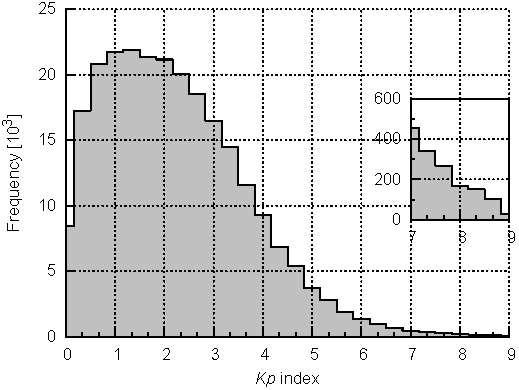
\includegraphics[width=0.46\textwidth]{figures_of_mine/chapter2/Kp_histogram_b.pdf}
		}{
			\caption{\Kp{} frequency distribution for the time period 1932--2016. The inset shows a zoomed-in view of the high-value tail. The \Kp{} data is obtained from the GFZ~Potsdam.}
			\label{fig:Kp_histogram_b}
		}
		\ffigbox{
			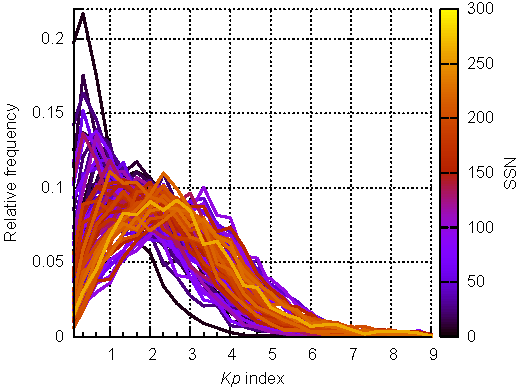
\includegraphics[width=0.95\Xhsize]{figures_of_mine/chapter2/Kp_histogram_yearlySSN_b.pdf}
		}{
			\caption{Yearly \Kp{} frequency distributions during the period 1932--2016, sorted and colored by yearly SSN. All distributions are normed to be of equal area. The \Kp{} data is obtained from the GFZ~Potsdam and the yearly SSN data from the SILSO World Data Center.}
			\label{fig:Kp_histogram_yearlySSN_b}
		}
	\end{floatrow}
\end{figure}

\subsection{Solar activity influence}
Obviously, the general \Kp{} distribution as seen in \autoref{fig:Kp_histogram_b} averages over solar activity. Solar activity is generally tracked with the international sunspot number (SSN). SSN data from the time period 1917--2016 is used in the present analyses. The data is obtained from the International Sunspot Number Monthly Bulletin and online catalog\footnote{WDC-SILSO website: \urlfoot{http://www.sidc.be/silso/}} provided by the World Data Center -- Sunspot Index and Long-term Solar Observations (WDC-SILSO), Solar Influences Data Analysis Center (SIDC), Royal Observatory of Belgium (ROB).

The \Kp{} frequency distributions' shape varies with solar activity (cite?). This is visible in the yearly distributions, sorted and colored by yearly SSN in \autoref{fig:Kp_histogram_yearlySSN_b}.

The distribution's peak position scales with SSN, that is, a high yearly SSN results in a higher abundance of large \Kp{} values as well (cite?).

The time series of yearly average \Kp{} values from the years 1932--2016 shows a solar cycle imprint, see the top graphs in \autoref{fig:yearly_kp-ssn_correlation_c}.
\begin{figure}
	\fcapside[\FBwidth]{
		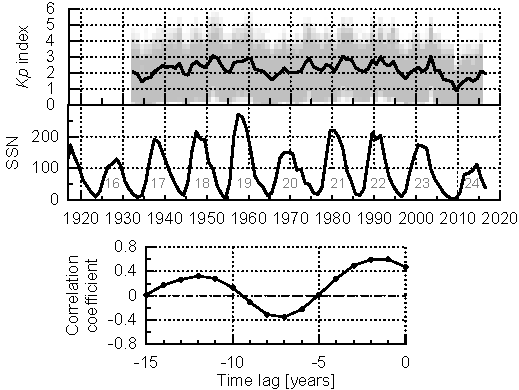
\includegraphics[width=0.6\textwidth]{figures_of_mine/chapter2/yearly_kp-ssn_correlation_c.pdf}
	}{
		\caption{Yearly \Kp~index distributions (shaded area) with their mean values for the time period 1932--2016 and yearly SSN with cycle number for the time period 1917--2016 (top panels). The Pearson correlation coefficients with the yearly SSN are calculated for time lags back to \num{-15}~years (bottom panel). The \Kp{} data is obtained from the GFZ~Potsdam and the yearly SSN data from the SILSO World Data Center.}
		\label{fig:yearly_kp-ssn_correlation_c}
	}
\end{figure}
The \Kp{} pattern follows the solar cycle minima and maxima as well as the changes in magnitude between solar cycles. The yearly mean \Kp{} shifts about 1~\Kp~unit for both variations separately. As expected, the correlation with solar activity shows an 11-year period, see bottom graph in \autoref{fig:yearly_kp-ssn_correlation_c}. The highest correlation coefficient of 0.60 is found with a time lag of $-1$~year, that is, the yearly average \Kp{} follows the SSN of the previous year.
%Kp-ssn cc: 0.5971

The yearly mean \Kp~index with respect to the 1-year lagged SSN shows a raise with increasing SSN, as seen from \autoref{fig:Kp_SSN_fit_d}.
\begin{figure}
	\fcapside[\FBwidth]{
		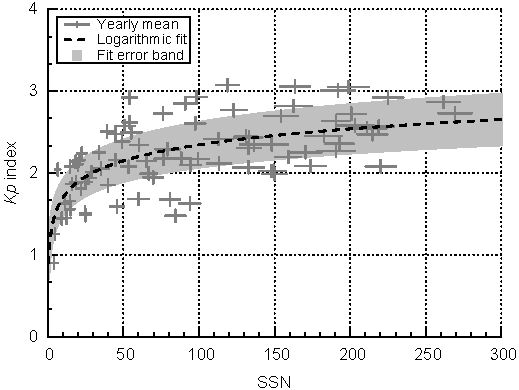
\includegraphics[width=0.6\textwidth]{figures_of_mine/chapter2/Kp_SSN_fit_d.pdf}
	}{
		\caption{Yearly mean \Kp~index with respect to 1-year lagged SSN (+) with the weighted logarithmic fit (dashed line). The error bars denote the SSN standard deviation and the relative weight from the yearly data coverage. The shaded area represents the fit error band derived from the estimated standard deviations of the fit parameters. The logarithmic function (\autoref{eq:log_fit_function}) is used for the weighted fit. The yearly \Kp{} mean values are calculated from GFZ~Potsdam data and the yearly SSN is obtained from the SILSO World Data Center.}
		\label{fig:Kp_SSN_fit_d}
	}
\end{figure}
In order to obtain an analytical relation for this dependency, I perform a least-squares regression fit. \Kp{} itself is a quasi-logarithmic index, so it is apparent to use a logarithmic fit function:
\begin{align}
	f(x) = a \cdot \ln(x) + b	\,.	\label{eq:log_fit_function}
\end{align}
The resulting fit parameters are $a = 0.281(43)$ and $b = 1.05(19)$; the numbers in parentheses are the estimated standard deviations.
They lead to the relation
\begin{align}
	\Kp(ssn) = 0.28 \cdot \ln(ssn) + 1.1	\,,	\label{eq:kp_ssn_relation}
\end{align}
% log fit parameters:
% a 0.281126         +/- 0.04267
% b 1.04923          +/- 0.19
which is plotted in \autoref{fig:Kp_SSN_fit_d}. This means that for an average yearly SSN of 1 the mean \Kp{} is $1.05(20)$ and for a SSN of 300 it is $2.65(31)$. The numbers in parentheses are the errors on the corresponding last digits of the quoted value. They are calculated via error propagation from the estimated standard deviations of the fit parameters.
% SSN	Kp	Kp_err
% 1	1.0492	0.189
% 10	1.6965	0.213
% 50	2.1489	0.252
% 100	2.3438	0.273
% 200	2.5387	0.295
% 300	2.6527	0.308

This relation is a practical resource for estimating the yearly average \Kp~index from the last year's average SSN. In 2017 the yearly SSN was \num{21.7(25)} -- applying this into the relation gives an average \Kp{} of \num{1.91} for 2018.

\subsection{Seasonal variations}
On top of the yearly variations, seasonal variations exist in the magnetospheric disturbances as well. In the months May--August the \Kp{} peak frequency is higher than in the remaining months of the year, whereas in March/April and September/October \Kp{} values larger than 3 are more abundant. This is apparent from looking at the monthly \Kp{} frequency distributions plotted in \autoref{fig:Kp_histogram_monthly}.
\begin{figure}[htb]
	\begin{floatrow}
		\ffigbox{
			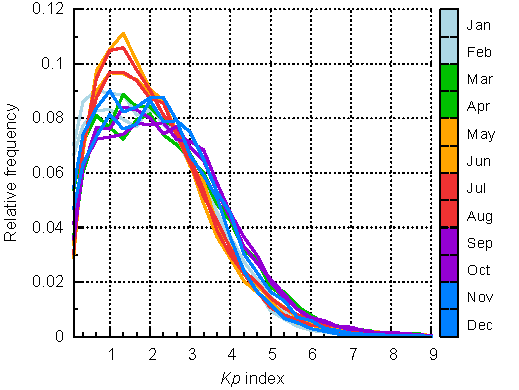
\includegraphics[width=0.46\textwidth]{figures_of_mine/chapter2/Kp_histogram_monthly.pdf}
		}{
			\caption{Average monthly \Kp{} frequency distributions of the time period 1932--2016, colored by month of the year. The \Kp{} data is obtained from the GFZ~Potsdam.}
			\label{fig:Kp_histogram_monthly}
		}
		\ffigbox{
			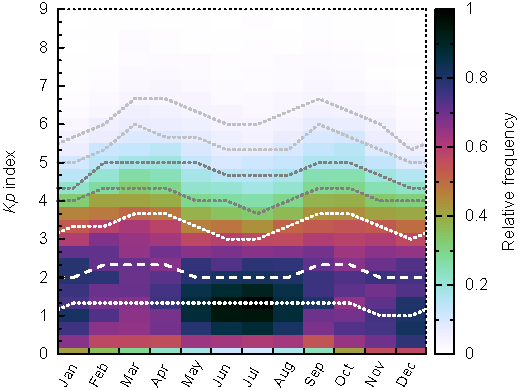
\includegraphics[width=0.46\textwidth]{figures_of_mine/chapter2/Kp_seasonal_e.pdf}
		}{
			\caption{\Kp{} frequency distributions by month for the time period 1932--2016 with median (white dashed) and quartile isolines (white dotted). The other dotted isolines mark the upper eighth, 16th, 32nd, and 64th parts. The bin size is 1~month and \SI{1/3}{\Kp}~unit respectively.}
			\label{fig:Kp_seasonal_e}
		}
	\end{floatrow}
\end{figure}
These \Kp{} changes arise from seasonal variations of the solar wind parameters at Earth, which stem from Earth's yearly changes in orbital distance and heliographic latitude. The Earth's rotation axis tilt adds another seasonal effect, the tilt changes the direction of the Earth's magnetic dipole axis to the Sun during the year.

Earth's distance to the Sun varies over the course of a year by \SI{+-1.67}{\percent}, see Appendix~\ref{sec:sun_earth_orbit_geometry}. The solar wind parameters scale via power-law dependencies with solar distance, as it is described in the following \autoref{chap:empirical_solar_wind_model_for_the_inner_heliosphere} and accordingly in \citet{Venzmer2018}. For example, the solar wind proton density scales with about $r^{-2}$, this leads to a yearly variation in density of about \SI{6.7}{\percent}. These yearly solar wind variations have direct influence on the \Kp{}~index.

The Sun's rotation axis tilt angle to the ecliptic is \SI{+-7.25}{\degree} and that for Earth is \SI{+-23.44}{\degree}, see also Appendix~\ref{sec:sun_earth_orbit_geometry}. The solar wind magnetic field strength varies with heliographic latitude (cite?). The solar wind influence on the \Kp{}~index depends on its coupling efficiency with the magnetosphere. Furthermore, the rate of magnetic reconnection between solar wind and the Earth's magnetosphere depends on both fields' orientation to each other (parallel/antiparallel). Additionally, the tilt of the magnetic dipole axis to the rotation axis -- only a few degrees for the Sun during cycle minima and extreme during solar maxima; and about \SI{10}{\degree} for the Earth -- complicates this system even more.
%geomagnetic dipole tilt: Planetary fact sheet: 11.2 (Model GSFC-12/83)
%variation range in the time period 1930--2016: 9.6--11.5° (http://wdc.kugi.kyoto-u.ac.jp/poles/polesexp.html)

So the \Kp{} variation effects originate from the seasonal change in the solar tilt, the Earth's tilt, and the Earth's solar distance. Thorough analyses of the seasonal variations were already early performed by \citet{Cortie1912} (more cites?). Thus, I just quantify the bulk magnitude of these effects in order to consider them as relative uncertainties when using the solar activity relation (\ref{eq:kp_ssn_relation}). Looking at the \Kp{} frequency distributions by month -- seen in \autoref{fig:Kp_seasonal_e} -- it is apparent that for high values ($\Kp{} > 4$), there exist yearly frequency maxima at the equinoxes and frequency minima at the solstices, as was early described by \citet{Cortie1912}. It is evident from the plotted quantiles that this semiannual variation amounts to $1/3$~\Kp~unit at small \Kp~values and up to 4/3~\Kp~units at higher \Kp~values.


\section{Relation between solar wind electric field and \Kp~index}
\label{sec:relation_between_sw_efield_and_kp}

\Kp{} nowcast from in-situ solar wind measurements at L1. Real-time solar wind make reliable measurements of all solar wind parameters available. It has a short lead-time and can therefore provide a nowcast.\\

The coupling between the solar wind and the magnetosphere is governed by reconnection and compression of the magnetic field lines, as described in \autoref{sec:solar_wind_coupling_mechanisms}. There exist quite a few coupling functions relating solar wind quantities with geomagnetic activity, see \autoref{sec:coupling_functions}. However, in this work I settle and work with the solar wind electric field as the coupling function. The reasons for using the electric field are that it is a simple coupling function and still reaches a high correlation...\\

% electric field
see \autoref{eq:coupling_vxBz}\\

The solar wind electric field y"~component $E_\text{y}$ approximates $\vect{E}$ under special circumstances, see derivation in \autoref{sec:electric_field_at_the_magnetopause}. It is the product of the radial proton velocity $v_\text{x}$ and the magnetic field z"~component $B_\text{z}$:
\begin{align}
	E_\text{y} = -v_\text{x} \, B_\text{z}\,.
\end{align}
If not specified otherwise, $B_\text{z}$ is always meant to be in GSM coordinates hereafter.\\


%velocity relation
The solar wind velocity sticks mostly to its radial flow direction, that is, it rarely deviates up to \SI{0.0}{\degree} (correct and cite...). Thus, the absolute flow speed $v$ can be used instead of the vector component.\\

argue for \vBz:\\
vs vBs vs vBT (Newell2007)\\
large northward fields still contribute to geomagnetic activity.\\
3hmin(\vBz) performs in rank correlation slightly better than the sophisticated Newell formula. really?\\


\subsection{Data correlation}
\label{sec:data_correlation}
%determine data basis
The \Kp{} time series started in 1932 when there existed no spacecraft to measure solar wind in~situ. Thus, the maximal surveyed time range is defined by the available in-situ solar wind data.\\

Savani2017:\\
``Although Kp is defined for 3 h periods, predicted variations in the IMF are made on shorter time scales and can influence the level of geomagnetic activity (e.g., geomagnetically induced currents). Hence, averaging the IMF over intervals that match those of Kp may suppress features that are important drivers of geomagnetic activity. Nevertheless, for the purpose of this paper, we choose to average the Kp estimate from the field vectors predicted by the BSS model over the same 3 h intervals as the Kp values, as this currently represents the service provided by NOAA/SWPC.''\\

Commonly the \Kp{} is estimated from 3-hour and 1-hour averages \citep{Savani2017} (more cites...).\\

%argue for averaging method
The \Kp{}~index represents maximal variations within 3-hour time intervals (see \autoref{sec:kp_index}). Any solar wind parameter that will be correlated with \Kp{}, obviously also has to have the same time resolution. In addition to adapting the time resolution, it has to be considered by which means this should be done. Simple 3-hour average values are expected to have a weaker correlation than the solar wind parameter's 3-hourly maximal variation.
%argue for high resolution, deliberate between hourly and minutely data
It is self-evident that the 3"~hour maximal variations are higher when using high resolution data. Thus, to be able to correlate \Kp{} with solar wind data in a proper way, high resolution data, that is, much shorter than the 3"~hour resolution, are needed to determine the maximal solar wind variations within each 3"~hour interval.\\

The OMNI data collection constitutes the longest continuous solar wind measurements made at \SI{1}{\au}. There exist two OMNI data sets with different time resolution -- the hourly version extends back to 1963 and the minutely version extends back to 1981. Although it is shorter, I choose to apply the minutely data, in order to benefit from the higher resolution. Thus, the work presented in this chapter is based on the minutely OMNI data set with a time duration spanning from 1981 until end of 2016.\\

vBz data...\\
The reduction to 3"~hour minimum values shifts the \vBz{} frequency distribution asymmetrically to negative values, whereas the averaged data is scattered around zero, see \autoref{fig:histogram_VBzgsm}.\\
\begin{figure}[htb]
	\begin{floatrow}
		\ffigbox{
			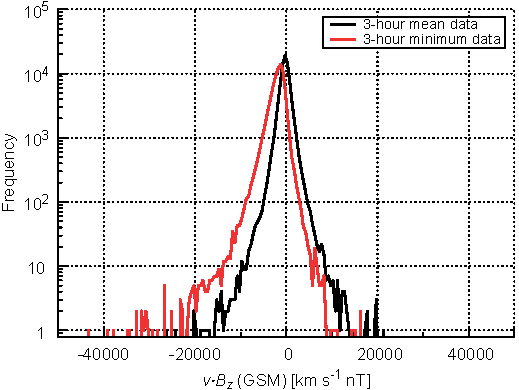
\includegraphics[width=0.46\textwidth]{figures_of_mine/chapter2/histogram_VBzgsm.pdf}
		}{
			\caption{Frequency distributions for the \vBz{} product. The minutely OMNI data from 1981--2016 is reduced to 3"~hour averages (black line) and 3"~hour minima (red line).}
			\label{fig:histogram_VBzgsm}
		}
%vBz frequency shifts:
% min shift: -1250
% mean shift: -250
% max shift: -750
		\ffigbox{
			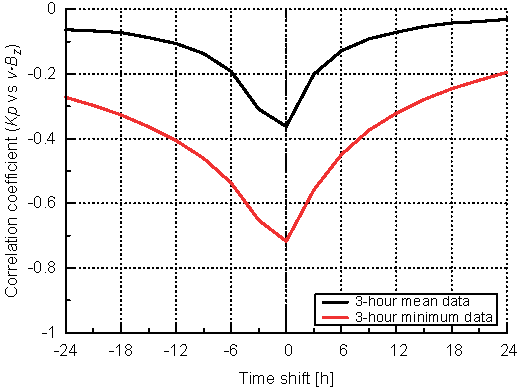
\includegraphics[width=0.46\textwidth]{figures_of_mine/chapter2/cc_lag_data_d_KpvsVBzgsm.pdf}
		}{
			\caption{\Kp--\vBz{} correlation coefficients for different time shifts up to \num{+-24}~hours. The minutely OMNI data from 1981--2016 is reduced to 3"~hour averages (black line) and 3"~hour minima (red line).}
			\label{fig:cc_lag_data_d_KpvsVBzgsm}
		}
%highest correlation coefficients:
%min:	0.00000    -0.717240
%mean:	0.00000    -0.362237
%max:	0.00000     0.293137
	\end{floatrow}
\end{figure}

The data is reduced to 3"~hour averages and 3"~hour minima in order to match the \Kp{} data resolution and evaluate the advantage of high resolution data. The \Kp{}--\vBz{} Pearson correlation coefficients for the two differently processed data versions are plotted over time shift in \autoref{fig:cc_lag_data_d_KpvsVBzgsm}. The data with 3"~hour minimum processing shows a much better correlation than the 3"~hour average data. Both curves show a negative correlation and their minima lie at a time shift of zero, with coefficients of $r_\text{min} = -0.72$ and $r_\text{avg} = -0.36$.

The best correlation at the time shift of zero is expected as the OMNI data represents the solar wind at the location of the magnetospheric bow shock. It takes the plasma only a couple of minutes to arrive at the magnetopause and influence the geomagnetic field.\\

Zhang2015 do with their data: ``The (OMNI) data have been lagged by 5~min to allow for propagation from the nose of bow shock to the magnetopause.''\\


\subsection{Functional dependency for solar wind electric field}
An empirical relation between \vBz{} and \Kp{} is sought by processing the data distribution and fitting an appropriate function to it.
%distribution
The frequency distribution in \Kp--\vBz{} space is shaped like a candle flame, inclined to negative values by a light breeze, see top panel in \autoref{fig:Kp_2dhistogram_VBzgsm_sws_e}. The negative correlation is already apparent.
\begin{figure}
	\fcapside[\FBwidth]{
		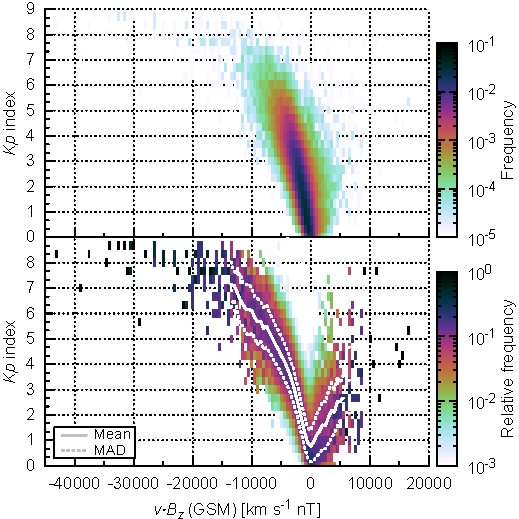
\includegraphics[width=0.6\textwidth]{figures_of_mine/chapter2/Kp_2dhistogram_VBzgsm_sws_e.pdf}
	}{
		\caption{\Kp{} versus \vBz{} frequency distribution (top panel) and its relative distribution (bottom panel) with the mean \Kp{} values (solid line) and their mean absolute deviation (dotted lines). It is 3-hour minimum data from the minutely OMNI data set (1981--2016). The bin size is \SI{500}{\km\per\s\nano\tesla} and \SI{1/3}{\Kp}~unit respectively.}
		\label{fig:Kp_2dhistogram_VBzgsm_sws_e}
	}
\end{figure}
%dependency
In order to determine a functional dependency, I focus on the relative frequencies per \vBz-interval and their mean \Kp{} values, which are plotted in the bottom panel of \autoref{fig:Kp_2dhistogram_VBzgsm_sws_e}. The mean absolute deviation (MAD) of the mean has a mean size of \SI{0.7}{\Kp}~units. This probability distribution is asymmetrically V-shaped around zero, having a larger and steeper negative arm than positive arm.
%MAD: 2.211/3 = 0.737 Kp units

The asymmetry also exists for 3"~hour mean data, thus this effect is not a result of the data reducing method (3-hour minimum). Rather the steeper negative arm is a consequence of the asymmetric coupling of the solar wind magnetic field direction to the magnetosphere, as described in \autoref{sec:solar_wind_coupling_mechanisms}.\\

%determine fitting functions
The appropriate type of function has to be constructed for the empirical fit. Since the \Kp~index has a quasi-logarithmic scaling (see \autoref{sec:kp_index}), a logarithmic function is the obvious choice as a fit function. Furthermore, the depending argument consists of a product of two solar wind parameters which individually scale logarithmically with \Kp{}. These reasons are why I use the logarithm of a parabola for the fitting approach:
\begin{align}
	f(x) &= \ln\left(x^2\right)	\,.	\label{eq:log_square_function}
\end{align}
I also introduce a horizontal shifting parameter $x'$ because the distribution's center is slightly offset. To be able to replicate the asymmetry in both arms, I further split the fit function at the minimum ($x + x'$) into arms of negative and positive slope:
\begin{align}
	f(x) &=
	\begin{cases}
		\,f_-(x) &\text{for } x + x' < 0	\,,\\
		\,f_+(x) &\text{for } x + x' \ge 0	\,.
	\end{cases}	\label{eq:log_square_fit_function}
\end{align}
This way, both arms can be scaled individually with scaling factors for the negative and positive parts $a_-$ and $a_+$. The resulting logarithmic fit function parts are
\begin{align}
	f_-(x) &= a_- \cdot \ln\left(\left(x + x'\right)^2 + b\right) + y'	\,,\\
	f_+(x) &= a_+ \cdot \left(f_-(x) - f_-\left(-x'\right)\right) + f_-\left(-x'\right)	\,,
\end{align}
with the vertical shifting parameter $y'$ and the depth parameter $b$. The resulting fit curve is plotted in \autoref{fig:Kp_2dhistogram_VBzgsm_sws_fit_e} with the fit coefficients $a_- = 1.258(19)$, $x' = 163(20)$, $b = \num{1.416(68)e6}$, $y' = -17.04(33)$, and \mbox{$a_+ = 0.467(20)$} for units of [\si{\km\per\s \nano\tesla}].
%high precision values:
% a_- = 1.25788(0.019)\\
% y' = -17.0394(0.33)\\
% a_+ = 0.467039(0.0197)\\
% b = 1.41639e6(0.067795e6)\\
% x' = 162.907(20.642)\\
\begin{figure}
	\fcapside[\FBwidth]{
		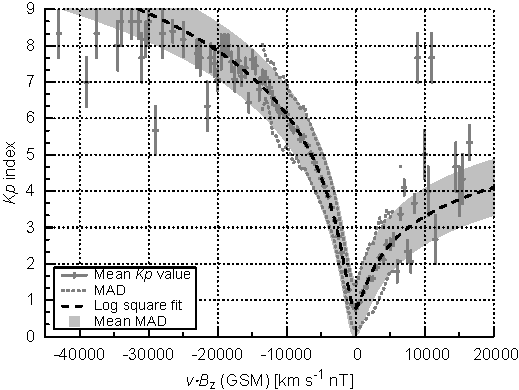
\includegraphics[width=0.6\textwidth]{figures_of_mine/chapter2/Kp_2dhistogram_VBzgsm_sws_fit_e.pdf}
	}{
		\caption{Mean \Kp{} values (+) and MAD values (dotted lines) per \vBz~interval. The error bars represent the relative data count. The logarithmic fit (dashed line) is plotted with a mean MAD band (shaded area). The splitted function (\ref{eq:log_square_fit_function}) is used for the weighted fit.}
		\label{fig:Kp_2dhistogram_VBzgsm_sws_fit_e}
	}
\end{figure}
Thus, the solar wind dependency relation 'condenses' to:
\begin{align}
	\text{\Kp}_-\left(vB_\text{z}\right) &= 1.258 \cdot \ln\left(\left(vB_\text{z} + 163\right)^2 + \num{1.416e6}\right) - 17.04	\,,	\label{eq:kpvsvbz_dependency_function_negative}\\
	\text{\Kp}_+\left(vB_\text{z}\right) &= 0.467 \cdot \left(\text{\Kp}_-\left(vB_\text{z}\right) - \text{\Kp}_-(-163)\right) + \text{\Kp}_-(-163)	\,.	\label{eq:kpvsvbz_dependency_function_positive}
\end{align}

% warning lead time
This derived E"~field relation can well be applied with the solar wind real-time measurements that are continuously being made by spacecraft located at L1, see \autoref{sec:solar_wind_nowcast_and_forecast_to_earth}. However, the heads-up time for warnings from this location is relatively short with a few tens of minutes, whereas remote observations via solar imagers and coronagraphs allow for longer lead times of a few days.

The E"~field relation derived above could also be applied to remote forecast situations, however, IMF strength and orientation are not yet properly predictable from current prediction methods that rely on remote observations.


\section{Relations between CME/stream velocities and \Kp~index}
\label{sec:relations_between_cme_stream_v_and_kp}

In order to still make use of the enhanced warning lead times from remote observations, the solar wind velocity is the only parameter left which is to a certain degree reliably forecastable. In fact, solar wind velocity and \Kp~index correlate quite well, \citet{Machol2013} even proposed a linear function of the \Kp~index as a best proxy for corrupted real-time velocity measurements made by the ACE spacecraft. For one, the velocity can even be used for persistence forecast, as it has the highest autocorrelation time of all major solar wind parameters -- with \SI{59}{\hour} it is much higher than that with the lowest autocorrelation time of \SI{4}{\hour}, which is indeed the $B_\text{z}$~GSM component \citep{Elliott2013}.

It is clear that the strength of the southward IMF component is the most dominant solar wind parameter for the driving of geomagnetic activity. The velocity shows a strong correlation during CME conditions as well, however, infact during HSSs the velocity is considered the most dominant parameter for driving the geomagnetic activity \citep{Holappa2014}.\\

% separating CMEs and streams
The distinct generation mechanisms of solar wind streams and CMEs show in their different appearance: streams are of continuous nature and CMEs are event-like. Therefore they require completely different forecast methods, see also \autoref{sec:solar_wind_nowcast_and_forecast_to_earth}. Thus, in order to forecast the \Kp~index from remotely derived velocity values, it is apparent and makes sense to analyze CMEs and solar wind streams separately.\\

% velocity relation
It is also known that the solar wind velocity itself already correlates strongly with the \Kp~index.\\

I use this velocity relationship for obtaining \Kp{} proxies from CME and solar wind stream data.\\


\subsection{Solar Wind Structures list}
For the separation of CME and stream data, I use the list of solar wind structures (SWS) created and updated by \citet{Richardson2000} and \citet{Richardson2012}. They characterized the near-Earth solar wind into periods related to slow wind, fast wind, and CMEs. Their list extends back to 1963 and is mostly based on 1"~hour averages of solar wind parameters from the OMNI data set. However, in the cases where there are gaps in the in-situ data, they consider other indicators for identifying solar wind structures. They achieve a fairly complete classification with the inclusion of data from geomagnetic activity, energetic particles, and cosmic rays.
Their work identifies solar wind structures and flags the time series into four categories: HSSs, slow solar wind, CME-associated flows, and undetermined intervals. Periods related to CMEs are defined to also comprise the associated ambient solar wind plasma, which consists of upstream shocks and compressed material. The criterion for differentiating between slow and fast solar wind is a velocity threshold of \SI{400}{\km\per\s}.

The SWS list is made available via registration at CEDARweb: \urltext{http://cedarweb.vsp.ucar.edu/wiki/index.php/Tools_and_Models:Solar_Wind_Structures}.
%List of near-Earth ICMEs since January 1996 by \citet{Cane2003,Richardson2010}. Available as ACE Level~3 data for the period 1995--mid2016\footnote{ACE Level~3 data website -- list of near-Earth ICMEs: \urlfoot{http://www.srl.caltech.edu/ACE/ASC/DATA/level3/icmetable2.htm}}.\\
The updated SWS list (until the end of 2016) was kindly provided by Ian~Richardson.

According to the SWS list, the CME fraction during the 36-year time period considered in the present study, 1981--2016, is \SI{15.4}{\%}, which accumulates to 5.53~years. %and that for the period 1963--2016 is \SI{16.9}{\%} (9.01~years).\\
This percentage is an average value, as the actual fraction varies heavily with the solar activity cycle and with the appearance of individual active regions on the solar surface.

In the following part of the study, I refer to the combination of the SWS categories slow and fast solar wind simply as solar wind streams. These periods are composed entirely from a mixture of slow wind flows, fast wind streams, and their interaction regions.


\subsection{Data correlation}
Again, as done before for the data processing of the E"~field analysis in \autoref{sec:data_correlation}, I calculate 3-hour extreme values using the minutely OMNI data in order to profit from the higher correlation. The comparison between the 3-hour maximum and the 3-hour mean frequency distributions shows that their mean positions are shifted slightly, having velocities of \SI{405}{\km\per\s} and \SI{425}{\km\per\s} respectively, as is shown in \autoref{fig:histogram_V_b}.
%the SWS1 mean raises from 435 to 455~km/s in 3hmax data...\\
\begin{figure}[htb]
	\begin{floatrow}
		\ffigbox{
			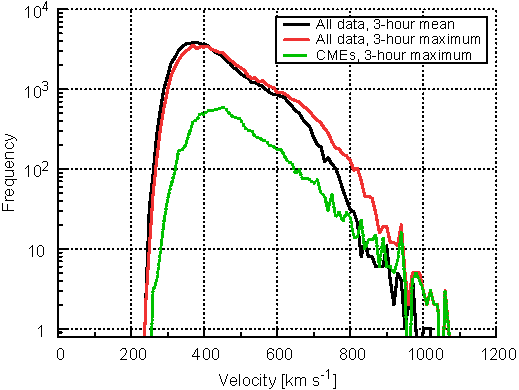
\includegraphics[width=0.5\Xhsize]{figures_of_mine/chapter2/histogram_V_b.pdf}
		}{
			\caption{Solar wind velocity frequency distributions for 3-hour mean, 3-hour maximum, and 3-hour maximum of the CME part. The minutely OMNI data from the period 1981--2016 is used.}
			\label{fig:histogram_V_b}
		}
		\ffigbox{
			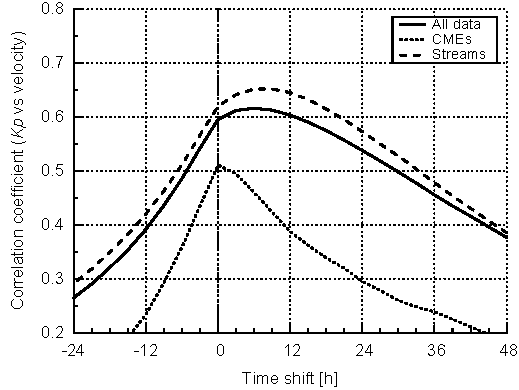
\includegraphics[width=\Xhsize]{figures_of_mine/chapter2/cc_lag_sws_d.pdf}
		}{
			\caption{\Kp{}--velocity correlation coefficients for time shifts in the range from $-24$ to 48~hours. The correlations are plotted for the whole solar wind data (solid line), for solar wind streams without CMEs (dashed line), and for CMEs only (dotted line). The data used is the 3-hour maximum of the minutely high resolution OMNI data from the period 1981--2016.}
			\label{fig:cc_lag_sws_d}
		}
	\end{floatrow}
\end{figure}
The CME part of the data is examined separately, filtering the related periods using the SWS list. The frequency distribution shows that the CME share is rising in faster solar wind, until eventually in the region above about \SI{900}{\km\per\s} there only exist CMEs.\\

The CME and stream parts of the data are correlated independently with the \Kp~index. The correlation for CME related data is lower than that for all solar wind, see \autoref{fig:cc_lag_sws_d}. Its maximal correlation coefficient has a value of 0.51 and is without time shift, see Table~\ref{tab:correlation_coefficients_kpvsv}.
\begin{table}
	\caption{Time lags with the highest correlation coefficients for the \Kp{}--velocity relation for all solar wind data, for stream data, and for CME data. The values are based on the 3-hour maximum of the minutely high resolution OMNI data from the time period 1981--2016.}
	\label{tab:correlation_coefficients_kpvsv}
	\centering
	\begin{tabular}{lcc}
		\hline\hline
		Data	&Time lag [hours]	&Correlation coefficient\\
		\hline
		All data	&6	&0.622\\
		Streams	&9	&0.661\\
		CMEs	&0	&0.511\\
		\hline
	\end{tabular}
\end{table}
% the best lag times are:\\
% sws: +6 h\\
% sws1: 0 h\\
% sws23: +9 h\\
% 
% correlation coefficients\\
% SWS1\\
% 0	0.511093\\
% SWS23\\
% lag	cross	auto x	auto y\\
% -3	0.660694\\
% 0	0.620113\\
% SWS\\
% lag	cross	auto x	auto y\\
% -2	0.621539\\
% 0	0.595784\\
Solar wind streams show a higher correlation with \Kp{} and the correlation's maximum value 0.66 has a positive time shift of 9~hours. That means the \Kp~index forecasts the velocity of solar wind streams 9~hours in advance.

This positive time shift can be explained from the occurence of interaction regions followed by HSSs. When a slow solar wind stream is followed by a fast one, the compression at their interface leads to enhanced solar wind densities and magnetic field strengths. The peak velocity of a HSS naturally appears after the interaction region. Therefore the \Kp-impact from the enhanced magnetic field is correlated with the higher velocity of the HSS, resulting in the observed positive time shift.\\


\subsection{Functional dependency for CME velocity}
The general \Kp--velocity dependency in the solar wind is apparent from the tilt of its distribution, see top panel of \autoref{fig:Kp_2dhistogram_V_sws_d}.
\begin{figure}
	\fcapside[\FBwidth]{
		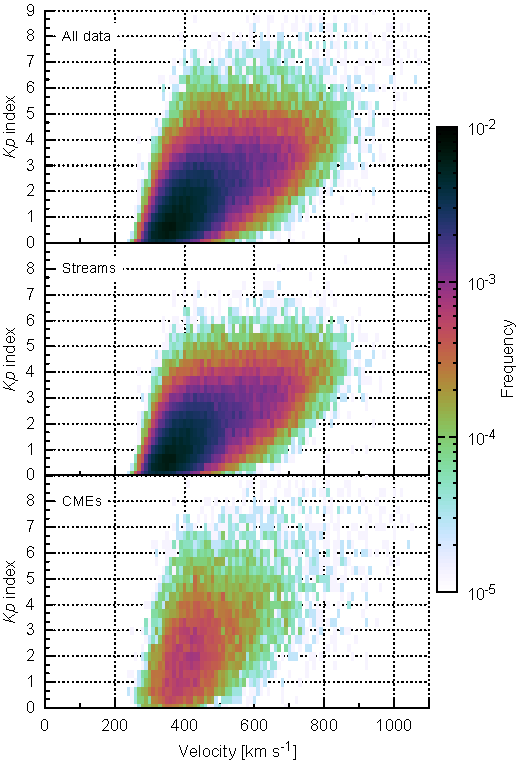
\includegraphics[width=0.6\textwidth]{figures_of_mine/chapter2/Kp_2dhistogram_V_sws_d.pdf}
	}{
		\caption{\Kp--velocity distributions for all solar wind data, for solar wind streams, and for CMEs. The data used is the 3"~hour maximum of the minutely high resolution OMNI data from the time period 1981--2016. The SWS list from \citet{Richardson2012} is used for the separation between CME and stream data. The bin size is \SI{10}{\km\per\s} and \SI{1/3}{\Kp}~unit respectively.}
		\label{fig:Kp_2dhistogram_V_sws_d}
	}
\end{figure}
The distribution is inclined to positive values but very broad, that is, in the typical solar wind velocity range it spans over more than half of the total \Kp{} range. The comparison with the filtered data shows that \Kp{} values \num{>6} and velocities \SI{>850}{\km\per\s} are almost always associated with CME related periods, see middle and bottom panel of \autoref{fig:Kp_2dhistogram_V_sws_d}.

In order to determine a functional relation between \Kp{} and velocity, I look at the relative \Kp{} frequencies for each \SI{10}{\km\per\s} velocity interval. The relative frequencies are plotted in the bottom panel of \autoref{fig:Kp_2dhistogram_V_sws1_c2}.
\begin{figure}
	\fcapside[\FBwidth]{
		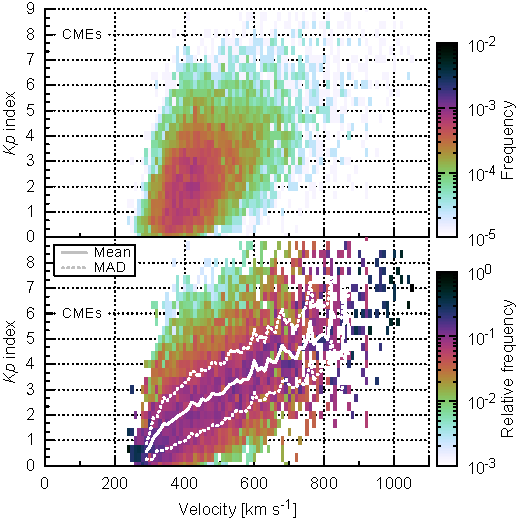
\includegraphics[width=0.6\textwidth]{figures_of_mine/chapter2/Kp_2dhistogram_V_sws1_c2.pdf}
	}{
		\caption{CME part of the \Kp--velocity distribution (same as third panel of \autoref{fig:Kp_2dhistogram_V_sws_d}) and its relative distribution per velocity interval with the mean \Kp{} values (solid line) and their mean absolute deviation (dotted lines). The bin size is \SI{10}{\km\per\s} and \SI{1/3}{\Kp}~unit respectively.}
		\label{fig:Kp_2dhistogram_V_sws1_c2}
	}
\end{figure}
The mean \Kp{} value seems to scale almost linear with the solar wind velocity. The MAD of the mean has a mean size of about \SI{1.1}{\Kp~units}.
%MAD: 3.338/3 = 1.113 Kp units

%determine fitting function
Again, as the \Kp~index has a quasi-logarithmic scaling, a logarithmic function is the obvious choice for the fitting process. Thus, the logarithmic function
\begin{align}
	f(x) = a \cdot \ln\left(x + x'\right) + y'	\label{eq:log_offset_fit_function}
\end{align}
is used for the fit, with the scaling factor $a$, the location parameter $x'$, and the vertical shifting parameter $y'$. The resulting fit is plotted in \autoref{fig:Kp_2dhistogram_V_sws1_fit_e} and its parameters are $a = \num{10.6(34)}$, $x' = \num{8.1(43)e2}$, and $y' = \num{-73(28)}$, with the velocity in units of [\si{\km\per\s}].
%10.6075 (3.4)\\
%-73.1694 (28.)\\
%806.943 (430)\\
\begin{figure}
	\fcapside[\FBwidth]{
		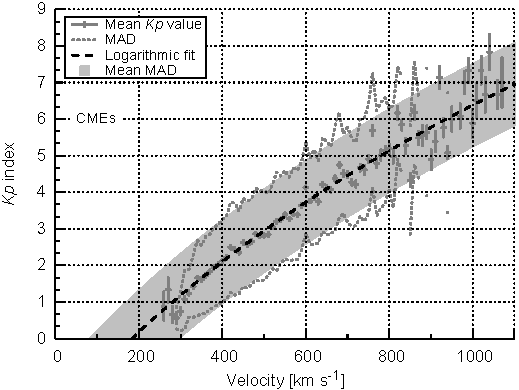
\includegraphics[width=0.6\textwidth]{figures_of_mine/chapter2/Kp_2dhistogram_V_sws1_fit_e.pdf}
	}{
		\caption{Mean \Kp{} values (+) and MAD values (dotted lines) per velocity interval for the CME part of the data. The error bars represent the relative data count. The logarithmic fit (dashed line) is plotted with a mean MAD band (shaded area). The function (\ref{eq:log_offset_fit_function}) is used for the weighted fit.}
		\label{fig:Kp_2dhistogram_V_sws1_fit_e}
	}
\end{figure}
This leads to the CME dependency function
\begin{align}
	\text{\Kp}_\text{CME}(v) = 10.6 \cdot \ln(v + 810) - 73	\,,	\label{eq:kpvsv_CME_dependency_function}
\end{align}
which can be used to forecast the \Kp{}~index from the estimated CME arrival velocity, e.g., obtained from analyses of remote coronagraph observations.


\subsection{Functional dependency for stream velocity}
The procedure in this section is the same as that in the previous section. However, in the case of solar wind stream velocities, the correlation coefficient is higher when the data is shifted by 9~hours, see \autoref{fig:cc_lag_sws_d}.
I use this shifted data and look at the relative frequencies per velocity interval in order to find a functional dependency between \Kp{} and velocity, see bottom panel of \autoref{fig:Kp_2dhistogram_V_sws23_d}.
\begin{figure}
	\fcapside[\FBwidth]{
		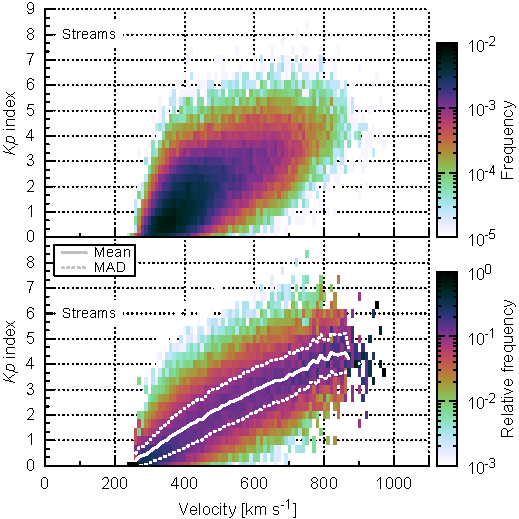
\includegraphics[width=0.6\textwidth]{figures_of_mine/chapter2/Kp_2dhistogram_V_sws23_d.pdf}
	}{
		\caption{Stream part of the \Kp--velocity distribution (similar to second panel of \autoref{fig:Kp_2dhistogram_V_sws_d}, but with the data shifted by 9~hours) and its relative distribution per velocity interval with the mean \Kp{} values (solid line) and their mean absolute deviation (dotted lines). The bin size is \SI{10}{\km\per\s} and \SI{1/3}{\Kp}~unit respectively.}
		\label{fig:Kp_2dhistogram_V_sws23_d}
	}
\end{figure}
Again, the mean \Kp{} value scales almost linear with the velocity. The distribution is much more narrower than that for CMEs -- the MAD of the mean has only a mean size of about \SI{0.7}{\Kp~units}.
%MAD: 2.226/3 = 0.742 Kp units
%MAD: 2.332/3 = 0.777 Kp units for 300--900km/s
%MAD: 2.389/3 = 0.796 Kp units for 350--900km/s
%MAD: 2.454/3 = 0.818 Kp units for 350--850km/s

%determine fitting function
Again, I use the logarithmic function (\ref{eq:log_offset_fit_function}) for the fitting process. The resulting fit is plotted in \autoref{fig:Kp_2dhistogram_V_sws23_fit_e} and the fit parameters are $a = \num{5.88(38)}$, $x' = \num{2.99(49)e2}$, and $y' = \num{-3.70(29)e1}$, with the velocity in units of [\si{\km\per\s}]. The MAD is about \SI{0.7}{\Kp}~units.
%a1 = 5.88(38)
%b1 = -37.0(29)
%x1 = 299(49)
\begin{figure}
	\fcapside[\FBwidth]{
		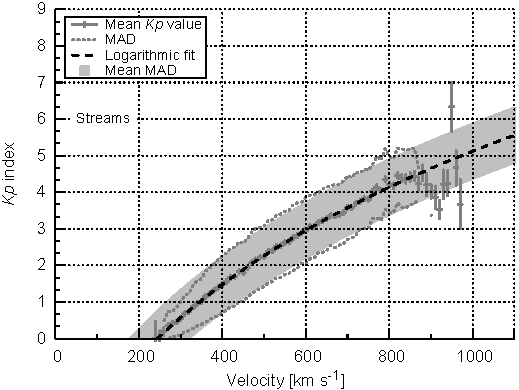
\includegraphics[width=0.6\textwidth]{figures_of_mine/chapter2/Kp_2dhistogram_V_sws23_fit_e.pdf}
	}{
		\caption{Mean \Kp{} values (+) and MAD values (dotted lines) per velocity interval for the stream part of the data, shifted by 9~hours. The error bars represent the relative data count. The logarithmic fit (dashed line) is plotted with a mean MAD band (shaded area). The function (\ref{eq:log_offset_fit_function}) is used for the weighted fit.}
		\label{fig:Kp_2dhistogram_V_sws23_fit_e}
	}
\end{figure}
This leads to the solar wind stream dependency function
\begin{align}
	\text{\Kp}_\text{Stream}(v) = 5.88 \cdot \ln(v + 299) - 37.0	\,,	\label{eq:kpvsv_stream_dependency_function}
\end{align}
which can be used to forecast the \Kp{}~index from the estimated stream velocity, e.g., obtained from remote coronal hole analyses.


\section{Prediction performance}
\label{sec:prediction_performance}
% prediction model performances
The derived empirical relations are chosen for their high correlation coefficients. However, the correlation coefficient itself does not represent the performance of a model as the coefficient depends highly on the scatter of the underlying distribution. Therefore \citet{Wing2005} advise to additionally provide scatterplots and skill scores for the evaluation of predictive models. In the following, I present the forecast errors and determine the true skill statistics as measures for the prediction performance of the drived empirical models.

% persistence
The quality of predictions can be assessed by how they compare to a simple persistence model \citep{Detman1999}. In the case at hand, the persistence consists of the official \Kp{} value from the previous 3"~hour interval.
% prediction performance
In order to evaluate the models' prediction performances, their forecast errors are calculated. Forecast errors are the differences between the predicted and the actual values. The resulting performances of the persistence and the three models are displayed in \autoref{fig:model_performance_c}, together with the corresponding standard deviations.
\begin{figure}
	\fcapside[\FBwidth]{
		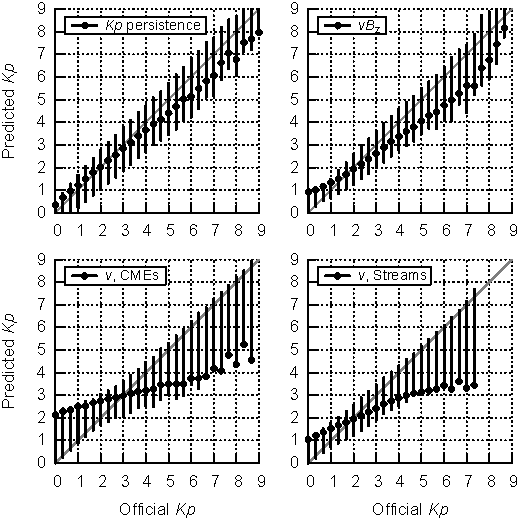
\includegraphics[width=0.6\textwidth]{figures_of_mine/chapter2/model_performance_c.pdf}
	}{
		\caption[\lofimage{figures_of_mine/chapter2/model_performance_c.pdf}]
		{Prediction performance of \Kp{} persistence and the three derived empirical \Kp{} relations. The forecast errors are the differences between the predicted and the actual values. They are calculated from the same data and time range as the relations themselves. The errorbars denote one positive and one negative standard deviation. Perfect predictions are indicated by the gray diagonal lines.}
		\label{fig:model_performance_c}
	}
\end{figure}
The persistence performance is obtained from the complete \Kp{} time span 1981--2016. It does fairly well, as its forecast error is less than 0.7~\Kp{} units up to a \Kp{} of 5.7. At and above a \Kp{} of 6 the error is underestimated with a maximum deviation of 1.3~\Kp{} units.

The derived empirical functions do not cover the whole \Kp{} range from 0 to 9 within the distributions of observed values. Only the \Kp{} values with more than one observed data point are considered for deriving the relations' prediction performances. This excludes the \Kp{}~9 values and in case of the velocity relation for streams also the values \Kp{}~7.7 and above.

% vBz performance
The derived \vBz{} function (\ref{eq:kpvsvbz_dependency_function_negative} + \ref{eq:kpvsvbz_dependency_function_positive}) does only coincide with significant data in the \Kp{} range 1 to 8.7. Especially because the minimum of the \vBz{} function is larger than 0.7~\Kp{}, as can be seen from \autoref{fig:Kp_2dhistogram_VBzgsm_sws_fit_e}. The model performs reasonably well at and below a \Kp{} of 5 with forecast errors smaller than 1~\Kp~unit. Larger \Kp~values are underestimated and deviate up to 1.7~\Kp~units from the predicted values.

% v CME performance
In the case of the velocity relation for CMEs, the derived function (\ref{eq:kpvsv_CME_dependency_function}) does only coincide with significant data in the \Kp{} range 1.3 to 6.3, as can be seen from \autoref{fig:Kp_2dhistogram_V_sws1_fit_e}. The magnitude is overestimated below a \Kp{} of 3 and underestimated above. In the range between a \Kp{} of 1 to 5 the forecast errors are smaller than 1.3~\Kp~units. Above, the error rises up to 4~\Kp~units at a \Kp{} of 8.7.

% v stream performance
For the velocity relation for streams, the derived function (\ref{eq:kpvsv_stream_dependency_function}) does only coincide with significant data in the \Kp{} range 0.3 to 4.3, as can be seen from \autoref{fig:Kp_2dhistogram_V_sws23_fit_e}. The magnitude is overestimated below a \Kp{} of 2 and underestimated above. The forecast errors are smaller than 1.3~\Kp~units throughout the valid range. Above, the error rises up to 4~\Kp~units at a \Kp{} of 7.3.

The model based on the \vBz{} relation is more accurate than those based purely on the velocity. This is expected, however, the \vBz{} relation is still eclipsed by the persistence model.\\

% true skill score
In order to further test the derived models for their predictive value, I derive their true skill statistic (TSS) -- a common tool for forecast verification. The TSS is a skill score based on the contingency table that categorizes forecasted and observed events. The score is the difference between the forecast hit rate and the false alarm rate. Its range goes from $-1$ to 1, where 1 indicates an ideal prediction and 0 a random prediction. I give a more detailed description on the TSS in the Appendix~\ref{sec:true_skill_statistic}. This method is the prevalent form of forecast verification in \Kp{} models \citep{Detman1999,Wing2005,Savani2017}. It is defined that each single 3"~hour \Kp{} interval represents an event and a hit occurs when both the forecasted and observed \Kp{} exceed a specified threshold. I adopt these criteria to make the results comparable. Therefore the TSS is derived as a function of \Kp{} threshold -- the results for persistence and the three models are plotted in \autoref{fig:true_skill_score}.
\begin{figure}
	\fcapside[\FBwidth]{
		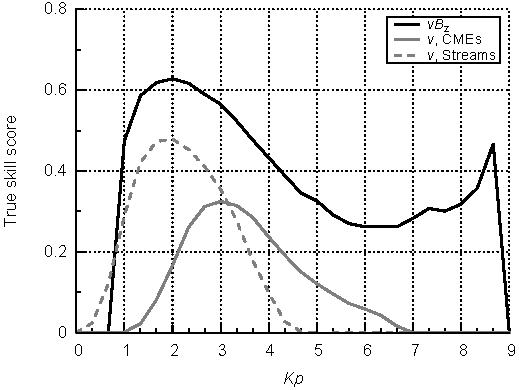
\includegraphics[width=0.6\textwidth]{figures_of_mine/chapter2/true_skill_score.pdf}
	}{
		\caption{True skill scores for the \Kp{} persistence and the three prediction relations as a function of \Kp{} threshold. The scores are calculated from the same data and time range as the relations themselves.}
		\label{fig:true_skill_score}
	}
\end{figure}

The E"~field relation reaches its peak at a \Kp{} of 2 with a TSS of 0.63, it then decreases to a local minimum at \Kp{} 6 with a TSS of 0.26. To higher \Kp{} values, the TSS increases again and reaches 0.47 at a \Kp{} of 8.7. This increase is due to the dominant number of correct null forecasts that make the TSS approach the hit rate \citep{Doswell1990}. It is a bias inherent to the TSS in case of rare event forecasting. Both velocity relations have throughout their \Kp{} ranges a significantly lower TSS. The CME relation shows a peak TSS of 0.32 at a \Kp{} of 3 and the stream relation a peak TSS of 0.48 at a \Kp{} of 2. Thus, the TSS gain from the additional $B_\text{z}$ component is about \numrange{0.15}{0.2}.\\

The persistence forecast clearly outperforms the other prediction models, especially in the high \Kp{} range. However, as \citet{Detman1999} stated, it has no warning value because it can only predict a high \Kp{} value after a high \Kp{} value was already observed. Thus, the persistence always misses the onset of a geomagnetic storm, whereas solar wind based models can provide at least a nowcast if not actually a short lead time from the distance of the in-situ measurement location at L1.

% statistics summary table
In order to compare the \Kp{} forecast skill metrics with other models, \citet{Savani2017} use a threshold of $\Kp{} \geq 5$. They choose this value because of the geomagnetic storm scale (G"~scale) developed by NOAA's SWPC. The G"~scale relates the \Kp~index to five levels from G1 to G5\footnote{NOAA Space Weather Scales website: \urlfoot{http://www.swpc.noaa.gov/noaa-scales-explanation}}. The starting level G1 translates to a \Kp{} of 5. I stick to this definition and provide a statistics summary of the \Kp{} persistence and the three derived models in \autoref{tab:model_statistics_table}.
\begin{table}[htb]
	\caption{Statistics of the different prediction models. The metrics are calculated for a threshold hit criteria of $\Kp{} \geq 5$ for the same data and time range as the relations themselves.}
	\label{tab:model_statistics_table}
	\centering
	\begin{tabular}{lcccc}
		\hline\hline
		\multirow{2}{*}{Parameter}	&\Kp{} persistence	&E"~field	&CME velocity 	&Stream velocity\\
			&$\Kp(t-1)$	&$\Kp(\text{\vBz})$	&$\Kp(v_\text{CME})$	&$\Kp(v_\text{Streams})$\\
		\hline
		Time shift [hours]	&3	&0	&0	&9\\
		Event count	&\num{105192}	&\num{79276}	&\num{12116}	&\num{65774}\\
		Correlation coefficient	&0.81	&\num{-0.72}	&0.51	&0.66\\
		\hline
		Proportion correct	&0.96	&0.97	&0.88	&0.98\\
		Hit rate	&0.55	&0.33	&0.13	&0\\
		False alarm rate	&0.02	&0	&0.01	&0\\
% 		FAR	&0.45	&0.24	&0.35	&1\\
% 		DFR	&0.02	&0.03	&0.11	&0.02\\
		True skill score	&0.53	&0.33	&0.12	&0\\
		Valid \Kp{} range	&\numrange{0.3}{8.7}	&\numrange{1.0}{8.7}	&\numrange{1.3}{6.3}	&\numrange{0.3}{4.3}\\
		\hline
	\end{tabular}
\end{table}
Obviously the defined \Kp{} threshold is of little use for the stream velocity relation as its valid \Kp~range is below the defining geomagnetic storm value of \Kp{} 5, that is, storms cannot be predicted via the stream relation.

% comparison
The E"~field model has a TSS of 0.33 at a \Kp{} of 5, this can be compared with the Wing APL models \citep[Fig.~13]{Wing2005}. The Wing APL model~3 predicts \Kp{} 1~hour in advance and uses the solar wind parameters velocity, density, magnetic field strength, and $B_\text{z}$ as input sources for a neural network based model. The additionally considered parameters (density and absolute magnetic field strength) boost the corresponding TSS to about 0.7. The Wing APL model~1 incorporates \Kp{} nowcast values in addition to the solar wind parameters and achieves this way a TSS of about 0.8.

The BSS model developed by \citet{Savani2015,Savani2017} predicts the magnetic field in CMEs arriving at Earth and derives their geomagnetic response. For a total of eight CME events the BSS model shows a TSS of 0.34, when investigating only the periods of ``active solar wind'' \citep[Tab.~3]{Savani2017}.
% Costello model (neural network, input: sw): about 0.45\\
% Wing APL model 1 (1 h, neural network, input: Kp nowcast + sw): about 0.8\\
% Wing APL model 2 (4 h, neural network, input: Kp nowcast + sw): about 0.7\\
% Wing APL model 3 (1 h, neural network, input: sw): about 0.7\\
% BSS model for eight CME events has $\mathit{TSS} = 0.34$ \citep[Tab.~3]{Savani2017}\\



\section{Discussion}
The following results are obtained from the \Kp{} analyses in this chapter:
\begin{itemize*}
	\item A functional dependency for the yearly \Kp{} averages that relates \Kp{} with solar activity via the SSN. The error to it is about 1/3~\Kp{}~unit, whereas seasonal variations further contribute up to 4/3~\Kp{}~units.
	\item A functional dependency for enabling a \Kp{} nowcast. It relates \Kp{} with the solar wind E"~field.
	\item A functional dependency for enabling a CME forecast. It relates \Kp{} with the velocity of CME-associated flows.
	\item A functional dependency for enabling a stream forecast. It relates \Kp{} with the velocity of solar wind streams.
\end{itemize*}


% extreme CME speeds
CMEs can be faster than the maximal velocities included in the OMNI data. Solar wind plasma spectrometers are only able to measure speeds up to about \SI{1100}{\km\per\s} reliably, leading to data gaps during these periods. Yet, CME speeds of up to \SI{2000}{\km\per\s} were observed at \SI{1}{\au} \citep{Russell2013}. According to \autoref{eq:kpvsv_CME_dependency_function}, a CME speed of this value would lead on average to a theoretical \Kp{} of 12.2, however, the \Kp{} scale is capped at 9o and a \Kp{} of 9o is reached already at a velocity of \SI{1489}{\km\per\s}, see \autoref{fig:Kp_2dhistogram_V_sws123_fit_f}.
% 2000 km/s -> 12.17~Kp
\begin{figure}
	\fcapside[\FBwidth]{
		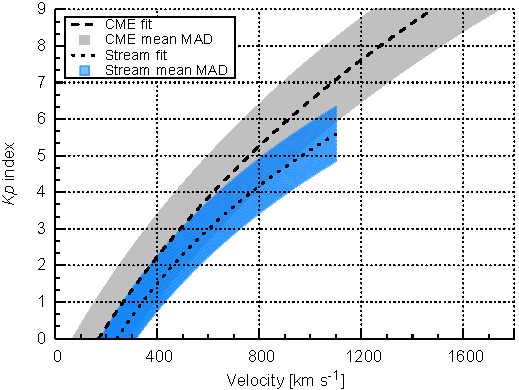
\includegraphics[width=0.6\textwidth]{figures_of_mine/chapter2/Kp_2dhistogram_V_sws123_fit_f.pdf}
	}{
		\caption{Logarithmic fit curves for CMEs (dashed line) and streams (dotted line) with their corresponding mean MAD bands (shaded areas). The curve for solar wind streams is cut because streams do not occur at these high velocities. The curves are the same as in Figures~\ref{fig:Kp_2dhistogram_V_sws23_fit_e} and \ref{fig:Kp_2dhistogram_V_sws23_fit_e}.}
		\label{fig:Kp_2dhistogram_V_sws123_fit_f}
	}
\end{figure}
Future studies have to show how accurate the CME relation is in predicting \Kp{} from extreme CMEs with velocities higher than \SI{1100}{\km\per\s}. (check with Niclas...)\\

The maximal velocity of regular solar wind is limited by the coronal temperatures \citep{Parker1958} and is observed to be around \SI{900}{\km\per\s}. That is why solar wind plasma associated with streams on average provoke \Kp{} values below 5o.\\

In order to demonstrate this relation with actual in-situ data, I calculate the \Kp{} estimate for the example CME from \autoref{fig:ACE_64s_v7_thesis_CME_2013-6-26_6} and include the 3"~hour minimum value of \vBz{} in the plot, see \autoref{fig:example_sw_plot_vBz_b_2013-6-26_6}.
\begin{figure}[htb]
	\centering
	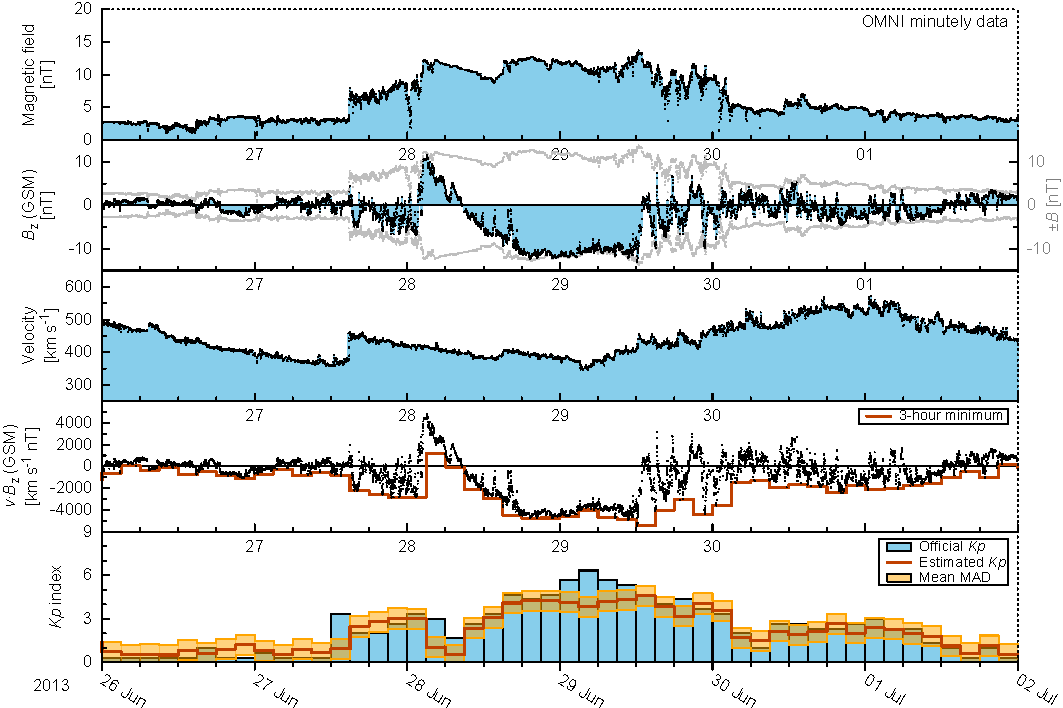
\includegraphics[width=\textwidth]{figures_of_mine/chapter2/example_sw_plot_vBz_b_2013-6-26_6.pdf}
	\caption[\lofimage{figures_of_mine/chapter2/example_sw_plot_vBz_b_2013-6-26_6.pdf}]
	{Solar wind measurements, official \Kp{}~index, and estimated \Kp{} for the time period from 26~June to 2~July 2013. The solar wind parameters are the magnetic field strength, its z"~component in GSM coordinates, and the velocity. I also plot the product \vBz{} with its 3"~hour minimum for illustration. The solar wind data are from the minutely OMNI data set. The official \Kp{}~index is obtained from the GFZ~Potsdam. The \Kp{} estimate is derived via Equations~\ref{eq:kpvsvbz_dependency_function_negative} and \ref{eq:kpvsvbz_dependency_function_negative}. The orange band indicates the mean MAD.}
	\label{fig:example_sw_plot_vBz_b_2013-6-26_6}
	\addtocontents{lof}{\smallskip\protect\center I created the figure myself.\medskip}
\end{figure}
It can be seen that in this period the \Kp{} estimate traces the actual \Kp{}~index pretty well within the mean MAD band. However, deviations are found at the times of the initial shock, and the start and middle of the MC.

It becomes obvious how important the influence of the magnetic field z"~component is, when looking at the same example CME from \autoref{fig:example_sw_plot_vBz_b_2013-6-26_6}. I plot its in-situ magnetic field strength and velocity in \autoref{fig:example_sw_plot_v_b_2013-6-26_6} together with the official \Kp{}~index and the derived \Kp{} estimate.
\begin{figure}[htb]
	\centering
	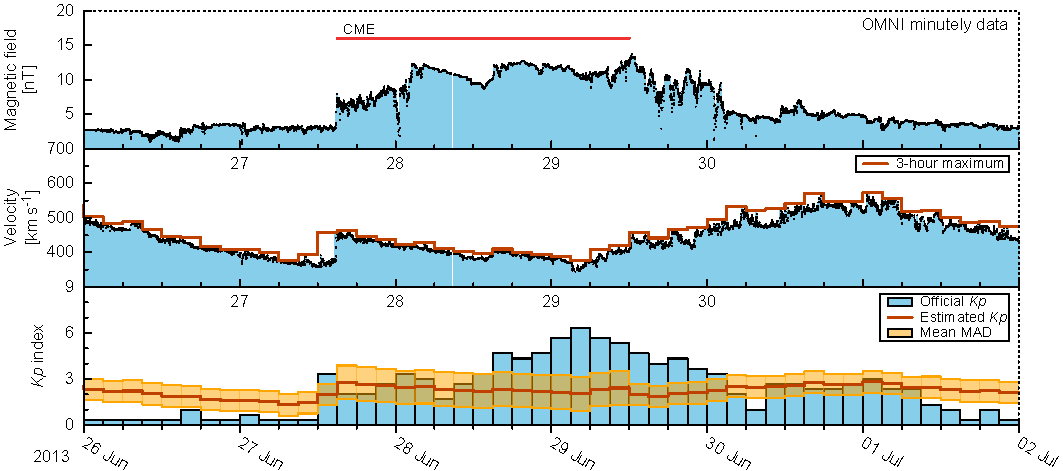
\includegraphics[width=\textwidth]{figures_of_mine/chapter2/example_sw_plot_v_b_2013-6-26_6.pdf}
	\caption[\lofimage{figures_of_mine/chapter2/example_sw_plot_v_b_2013-6-26_6.pdf}]
	{Solar wind measurements, official \Kp{}~index, and estimated \Kp{} for the time period 26~June to 2~July 2013. The solar wind parameters are the magnetic field strength and the velocity. I also plotted the velocity's 3"~hour maximum for illustration. The solar wind data are from the minutely OMNI data set. The official \Kp{}~index is obtained from the GFZ~Potsdam. I plot the \Kp{} estimate depending on whether the period is flagged as a CME in the SWS list (red line in top panel) or not, that is, via \autoref{eq:kpvsv_CME_dependency_function} or \autoref{eq:kpvsv_stream_dependency_function}. The orange band indicates the mean MAD.}
	\label{fig:example_sw_plot_v_b_2013-6-26_6}
	\addtocontents{lof}{\smallskip\protect\center I created the figure myself.\medskip}
\end{figure}
The latter do not coincide well during this period. The \Kp{} estimate performs okay during the initial sheath region and around the peak of the trailing HSS. The rarefaction regions of declining velocity at the start and end of the considered interval are overestimated, whereas the MC and the trailing compression region are underestimated.

solar wind stream example in \autoref{fig:example_sw_plot_v_c_2013-5-1_65}\\
\begin{figure}[htb]
	\centering
	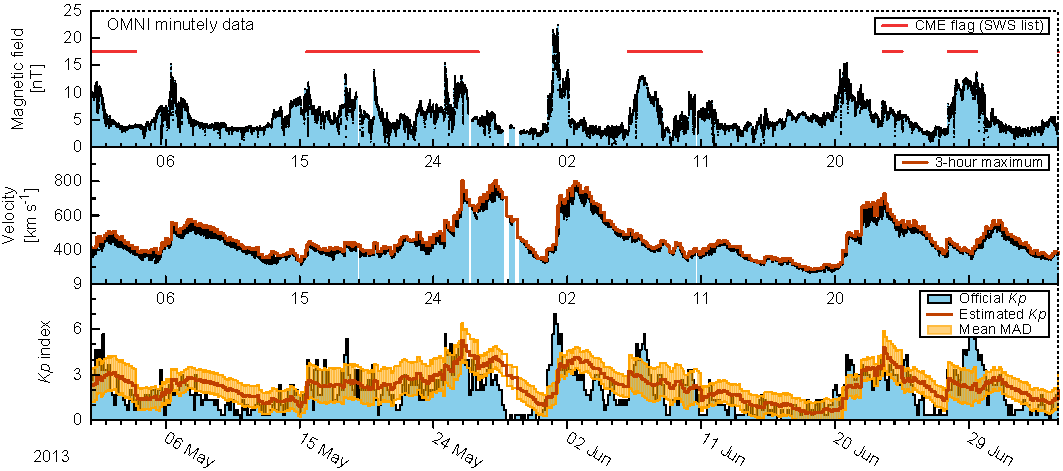
\includegraphics[width=\textwidth]{figures_of_mine/chapter2/example_sw_plot_v_c_2013-5-1_65.pdf}
	\caption[\lofimage{figures_of_mine/chapter2/example_sw_plot_v_c_2013-5-1_65.pdf}]
	{Solar wind measurements, official \Kp{}~index, and estimated \Kp{} for the time period 1~May to 5~July 2013. The solar wind parameters are the magnetic field strength and the velocity. I also plotted the velocity's 3"~hour maximum for illustration. The solar wind data are from the minutely OMNI data set. The official \Kp{}~index is obtained from the GFZ~Potsdam. I plotted the \Kp{} estimate depending on whether the period is flagged as a CME in the SWS list (red line in top panel) or not, that is, via \autoref{eq:kpvsv_CME_dependency_function} or \autoref{eq:kpvsv_stream_dependency_function}. The orange band indicates the mean MAD.}
	\label{fig:example_sw_plot_v_c_2013-5-1_65}
	\addtocontents{lof}{\smallskip\protect\center I created the figure myself.\medskip}
\end{figure}


The present study adds more empirical \Kp{} relations -- for the specific forecast situations when only the solar wind velocity $v$ or its E"~field are obtainable.\\

differences to existing studies -> Elliott2013\\
It can be looked at how well the solar wind stream velocity relation compares to the compression/rarefaction relations derived by \citet{Elliott2013}.\\

comparison:\\
\Kp--velocity correlation\\
similar to \citet{Elliott2013}; different data time period, resolution and averaging method (3-hour maximum of 1~min data)\\
see Akasofu1981 p.~126, table\\


\section{Applications and outlook}

\subsection*{Applications}
Prototype \Kp{} relations are integrated into applications developed within the Advanced Forecast For Ensuring Communications Through Space (\mbox{AFFECTS}) project which ran from 2011 to 2013. The following services are accessible via the \mbox{AFFECTS} website\footnote{AFFECTS website: \urlfoot{http://www.affects-fp7.eu/services/}} and contain early results from this \Kp{} study:
\begin{itemize*}
	\item Real-time solar wind plot: \href{http://www.affects-fp7.eu/rssfeeds/ace_ap_forecast_plot/ace_realtime_ap_CH_GFT_plot.png}{Solar Wind and \Kp{} forecast plot} -- ACE/DSCOVR real-time solar wind and \Kp{} forecast plot.
	\item RSS feed: \href{http://www.affects-fp7.eu/rssfeeds/rssfeed_kp/rssfeed_kp.xml}{L1 Kp Alert} -- threshold-based RSS feed that gets triggered when the estimated \Kp{} surpasses a threshold specified as being $7-$.
	\item RSS feed: \href{http://www.affects-fp7.eu/rssfeeds/rssfeed_gnss/rssfeed_gnss.xml}{L1 GNSS Alert} -- threshold-based RSS feed that gets triggered when a specified GNSS error is reached. The value is derived from the \Kp{} estimate.
	\item RSS feed: \href{http://www.affects-fp7.eu/rssfeeds/rssfeed_aurora/rssfeed_aurora.xml}{L1 Aurora Alert} -- threshold-based RSS feed that gets triggered when a specified auroral location is reached. The value is derived from the \Kp{} estimate.
\end{itemize*}

\noindent Further applications of the derived \Kp{}-relations:
\begin{itemize*}
	\item The derived \Kp{} relations are integrated into the UGOE/IAG CME forecast chain (DDC), which consists of CME source region and coronal environment analysis, 3D modeling of the CME structure, CME acceleration and propagation modeling, CME arrival time and parameter prediction, and the subsequent forecast of relevant space weather quantities, such as its impact on the \Kp~index and the ionospheric TEC.
	\item iPhone app L1 Alerts (Solar wind latest 2-hour extreme values and derived forecast values):\\
	\urltext{http://www.affects-fp7.eu/app-services/L1-Alerts/dataL1Alerts.txt}\\
	\urltext{https://itunes.apple.com/au/app/affects/id893579846}
% 	\item Android app L1 Alerts... \urltext{https://play.google.com/store/apps/details?id=com.afects.forecasts}
	\item has SW-Display Kp forecast??
\end{itemize*}


\subsection*{Outlook}

In the present study, the solar activity is neglected for deriving the empirical solar wind--\Kp{} relations. It would be worth examining the solar cycle's influence on the relations, especially as \citet{Wing2005} note that the predictability of \Kp{} slightly scales with solar activity.\\

% low solar activity influence on geomagnetic storms/space weather
\textit{The weaker solar activity cycle 24 seems to have important consequences for CMEs in the heliosphere: CMEs expand anomalously due to reduced heliospheric pressure leading to the increased observed rate of small CMEs, halos originating far from the disk center, and mild space weather (\citep{Gopalswamy2014}, 2015a; Petrie 2015).\\
The total pressure in the heliosphere (magnetic + plasma) is reduced by ca. 40\%, which leads to the anomalous expansion of CMEs explaining the increased slope. The excess CME expansion contributes to the diminished effectiveness of CMEs in producing magnetic storms during cycle 24, both because the magnetic content of the CMEs is diluted and also because of the weaker ambient fields \citep{Gopalswamy2014}.\\
}
maybe the derived relations are less valid during these current conditions?\\

Separate small-scale solar wind structures, such as CIRs and HCSs, for their \Kp{} impact. Filter CME-associated flows into their substructures, such as compressed solar wind plasma and MC plasma, and evaluate their \Kp{} impact individually.\\

\bigskip
{\small
\textit{Acknowledgments.} Part of the research leading to the results presented in this chapter has received funding from the EU~FP7 project AFFECTS under grant 263506.
The analyses in this chapter rely on the \Kp~index, calculated and made available by the GFZ~Potsdam from data collected at magnetic observatories. Thank goes to the involved national institutes, the INTERMAGNET network and ISGI (\urltext{isgi.unistra.fr}). The author thanks the WDC-SILSO at the SIDC (ROB) for maintaining and providing the international sunspot number series. Additional thank gos to the OMNI PIs/teams for creating and making available the solar wind in-situ data. The OMNI data are supplied by the SPDF at GSFC (NASA). The hourly SWS list, updated until the end of 2016, was kindly provided by Ian~Richardson of the GSFC and CRESST/University of Maryland.
}

\section*{notes...}

Savani2017:\\
The Kp difference of 1.5 is tested as there is evidence that a limitation in accuracy is present in the underlying empirical Kp formulation [Mays et al., 2015a]. [...] which is approximately consistent with recent results by Mays et al. [2015a], the Kp empirical formulation is accurate to about Kp = 1.5.\\

What kind of solar wind structures create the individual regions in this distribution? (B--v--\Kp{} circle plot)\\
What is their individual contribution to the \Kp{} ranges (e.g. high \Kp{}: CMEs 70\% and CIRs 30\%)?\\

How can the impact field strength of CMEs be forecasted (v->B correlation for CMEs)?\\
Internal solar wind correlations: B--v correlation\\
ACE MAGSWE 64~s data -> yearly overlay plot\\

Using \vBz{} implies that both quantities are sufficiently independent. $B$ and $v$ are dependent, as can be seen from fig~XX, however, as $v$ and $\theta_c$ are, so are $v$ and $B_\text{z}$, see fig~XX.\\

rt data errors/gaps... vs science data (see paper Kp as V replacement: \citet{Machol2013})\\
DSCOVR as replacement was launched on 11~Februar 2015. It is NOAA's SWPC real-time solar wind prime source since 27 July 2016.\footnote{\urlfoot{http://www.swpc.noaa.gov/products/real-time-solar wind}}\\




	\chapter{Solar wind time variations}
\section{Solar wind variation with solar cycle}
\section{Solar wind variation with season}
\section{Solar wind empirical forecast}

\chapter{Solar wind distance variations}
\section{Solar wind back-extrapolation}


%COFI -- chapter outline and flow integration\\

see paper...\\

McGregor2011 analyzed the empirical magnetic topology–velocity relationship, using Helios perihelion data with the Wang-Sheeley-Arge (WSA) coronal model, and found indications, that the fast and slow solar wind are generated from distinct sources. (not only superradial expansion)\\


	
	%####--  PaperMVVB  --####
	
\autoref{sec:frequency_distributions_of_the_solar_wind_parameters}\\
replace paper with actual published A\&A version...\\
\includepdf[openright,addtotoc={
1,chapter,1,Paper: Solar-wind predictions for the Parker Solar Probe orbit,chap:solar_wind_predictions_for_the_parker_solar_probe_orbit,
1,subsection,3,Abstract,sec:abstract,
1,section,2,Introduction,sec:introduction,
2,section,2,Frequency distributions of the solar-wind parameters,sec:frequency_distributions_of_the_solar_wind_parameters,
3,section,2,Solar activity dependence of the solar-wind frequency distributions,sec:solar_activity_dependence_of_the_solar_wind_frequency_distributions,
6,section,2,Solar distance dependency,sec:solar_distance_dependency,
9,section,2,Empirical solar-wind model,sec:empirical_solar_wind_model,
10,section,2,Model extrapolation to PSP orbit,sec:model_extrapolation_to_psp_orbit,
12,section,2,Discussion and summary,sec:discussion_and_summary,
13,subsection,3,References,sec:references
},pages={-}]{paperMVVB/aa31831-17.pdf}

%paper issue: first page toc links wrong because of openright

	%%\chapter{PaperMVVB}
%\section{Abstract}

\titley{Solar wind and CME influence on the magnetosphere}
\subtitley{Impact estimations derived from empirical correlations between in~situ solar-wind measurements and the geomagnetic \Kp{}~index}

% \author{M.~S.~Venzmer}
% 
% \institute{University of Goettingen, Institute for Astrophysics, Friedrich-Hund-Platz~1, 37077~Göttingen, Germany}
% 
% \date{First draft 28 April 2017; received date; accepted date }

\abstracty
{Variations in the Earth's magnetosphere are largely evoked by influence through the solar wind. These magnetospheric disturbances have diverse effects on the terrestrial environment. Especially the effects of severe geomagnetic storms created by coronal mass ejections (CMEs) pose various threats to sensitive technical systems and exposed humans. Thus, the development of quantitative forecasts for magnetospheric impacts caused by solar wind and CMEs is very important.}	%context
{This study's goals are to estimate the magnetospheric impact from solar activity in general, from solar wind and also to predict it for CMEs in particular. We present empirical dependencies between specific solar-wind parameters and the magnetospheric disturbance index~\Kp{}. These dependencies allow to nowcast the \Kp~index from upstream (L1) solar-wind in situ measurements. Hence, also the magnetospheric impact of CMEs is estimated solely based on their arrival velocities, predicted from coronagraphic observations. The prediction of solar-wind stream velocities from coronal hole (CH) observations, enables to estimate their impact as well.}	%aims
{First, we estimate the long-term variations of the yearly average \Kp{}~values, which are contributed by solar activity. This is achieved via logarithmic fitting of a yearly sunspot number (SSN) dependency. For the \Kp{} nowcast from general solar-wind conditions, we use a correlation with the product of the parameters velocity and magnetic field z\~component in GSM coordinates (\vBz{}). For the \Kp{} forecast from estimated CME and stream velocities, we furthermore filter the solar-wind data using flagged CME times from the solar-wind structures (SWS) list provided by \citet{Richardson2012}. The solar-wind data considered in our analyses consists of 35~years (1981--2016) of high-resolution minutely OMNI data, which is composed of multi-spacecraft intercalibrated in situ measurements from \SI{1}{\au}. We evaluate various data processing methods and choose the methods resulting in the highest correlation coefficients with \Kp{}. We analyze the \Kp{} frequency distributions with respect to the depending parameters \vBz{} and velocity, derive their mean \Kp{} per interval and further compile functional dependencies via logarithmic fitting.}	%methods
{The obtained functional relations enable us to empirically estimate the mean \Kp{} impact from measured solar activity, in situ solar wind, and remotely observed CHs and CMEs.}	%results
{}	%conclusions

% \keywords{solar wind -- sun: coronal mass ejections (CMEs) -- earth}
% 
% \maketitle

%\tableofcontents

\section{Introduction}
%motivation
It is long known (since the early 19th~century) that variations in the solar wind evoke disturbances in the magnetosphere \citep{Bartels1962}. Especially strong disturbances, called geomagnetic storms, can be provoked by coronal mass ejections (CMEs), which are embedded within the solar wind. The causes of the strongest geomagnetic storms are the compression of the solar wind magnetic field lines within the CME shock front and the in CMEs enclosed magnetic clouds with their enhanced field strenghts \citep{Bothmer1993}.

These strong geomagnetic disturbances are a threat to sensitive technical systems and exposed humans. Therefore it is important to know when magnetospheric disturbances will occur and how large they will be.\\

%aim
The goal of this paper is to estimate the magnetospheric impact of solar wind in general and to predict it for CMEs in particular.\\


%outline of structure
First we determine the magnitudes of the long-time \Kp{} changes due to solar activity (Sect.~...) and second we measure the extent of seasonal variations stemming from the Earth's orbit (Sect.~...).\\

%general solar wind nowcast
In situ measurements of solar wind are made almost continuously (e.g., at the first Lagrange point (L1)) in front of the magnetosphere. Since 1963 several spacecraft collected more than 50~years of data. The latest spacecraft, e.g., Wind, ACE and DSCOVR (launched in early 2015), provide real-time solar wind data.\footnote{Wind: \url{https://pwg.gsfc.nasa.gov/windnrt/}} \footnote{ACE: \url{http://www.swpc.noaa.gov/products/ace-real-time-solar-wind}} \footnote{DSCOVR: \url{http://www.swpc.noaa.gov/products/real-time-solar-wind}}

This real-time data can be used to estimate various solar wind effects, e.g., the position of the magnetospheric bow shock in front of the Earth, the magnitude of geomagnetic disturbances (\Kp~index), the positions of the polar auroral ovals, the variation of the total electron content (TEC) of the ionosphere, the positional error of global navigation satellite systems (GNSS),...\\

The equatorward auroral boundary position correlates with the \Kp~index.\\

The total electron content (TEC) of the ionosphere has influence on global navigation satellite systems (GNSS). A part of their positional error scales directly with the TEC (in extreme cases up to about \SI{30}{\m}).\\

%CME velocity forecast
The velocity and direction of CMEs can be determined in their early near\~Sun stages via remote tracking with coronagraph white-light observations. Using these parameters as input for propagation models, their possible arrival time and arrival velocity at Earth can be derived.\\

%stream velocity forecast from CHs
As coronal holes are the origin of the fast solar wind, their area on the solar disk, seen in EUV images, correlates with the measured velocity of solar wind streams \citep{Vrsnak2007}. This is used to predict the Earth arrival velocity of solar wind streams about 4~days in advance \citep{Rotter2012}.\footnote{\url{http://swe.uni-graz.at/index.php/services/solar-wind-forecast}}\\

With our results presented here we elaborate the step from the predicted CME and stream velocities to the forecast of the possible impact strength on the Earth's magnetosphere.\\

%differences to existing studies
[\citet{Elliott2013}: The \Kp~index and solar wind speed relationship: Insights for improving space weather forecasts]\\

We make an empirical correlation of the solar wind speed with the geomagnetic \Kp~index to obtain the capability to forecast \Kp{} values solely based on the predicted CME and stream velocities.\\

The used OMNI data set consists of minutely data in the time range 1981-01-01 to 2016-12-31.\\

The derived functional dependencies can be used to nowcast/forecast the \Kp~index.\\


%motivation
why use the \Kp{} index?\\


\section{Long-term variations of the \Kp{}~index}

\subsection{\Kp{} data}
The \Kp{} data is obtained from the GFZ~Potsdam\footnote{\url{http://www.gfz-potsdam.de/de/kp-index/}}, where the index is now maintained. The data used in this analysis covers the time period 1932--2016.\\

The \Kp{} frequency distribution for the time period 1932--2016 shows that the highest frequencies occur around low \Kp{} values of 1+ and to higher \Kp{} values the frequencies seem to decline exponentially (see Fig.~\ref{fig:Kp_histogram}). A \Kp{} value of 9o occurred only 29 times in this time interval.\\
\begin{figure}
	\fcapside[\FBwidth]{
		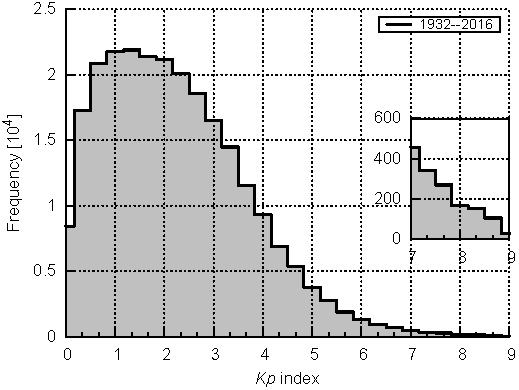
\includegraphics[width=0.5\textwidth]{chapter2/figures/Kp_histogram.pdf}
	}{
		\caption{\Kp{} frequency distribution for the time period 1932--2016. \Kp{} data from the GFZ~Potsdam.}
		\label{fig:Kp_histogram}
	}
\end{figure}

\subsection{\Kp{} variations with solar activity}
solar activity is tracked with the sunspot number (SSN); SSN data\\
The general \Kp{} distribution, seen before in Fig.~\ref{fig:Kp_histogram}, averages over solar activity. With different states of solar activity the \Kp{} frequency distributions' shape varies. This can be seen from the yearly distributions, sorted and colored by yearly SSN (see Fig.~\ref{fig:Kp_histogram_yearlySSN}). The distribution's peak position scales with SSN, that is, a high yearly SSN results also in more large \Kp{} values.\\
\begin{figure}
	\fcapside[\FBwidth]{
		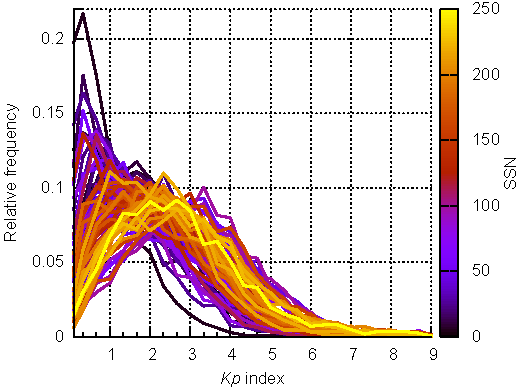
\includegraphics[width=0.5\textwidth]{chapter2/figures/Kp_histogram_yearlySSN.pdf}
	}{
		\caption{Yearly \Kp{} frequency distributions of the period 1932--2016 sorted and colored by SSN. \Kp{} data from the GFZ~Potsdam and the yearly SSN from the SILSO World Data Center.}
		\label{fig:Kp_histogram_yearlySSN}
	}
\end{figure}

The time series of yearly average \Kp{} values in the time span 1932--2016 shows an imprint of the solar cycles (see the top graphs in Fig.~\ref{fig:yearly_kp-ssn_correlation_c}).
\begin{figure}
	\fcapside[\FBwidth]{
		\includegraphics[width=0.5\textwidth]{chapter2/figures/yearly_kp-ssn_correlation_c.pdf}
	}{
		\caption{Yearly \Kp~index from GFZ~Potsdam and yearly SSN from the SILSO World Data Center (1932--2016) with cycle number (top). The correlation coefficients with the yearly SSN are calculated for time lags back to -15~years (bottom).}
		\label{fig:yearly_kp-ssn_correlation_c}
	}
\end{figure}
The \Kp{} pattern follows the solar cycle minima and maxima as well as the changes in magnitude between solar cycles. The yearly mean \Kp{} shifts about 1~unit for both variations.

As expected, the \Kp{}~index correlation with solar activity shows an 11-year period (see bottom graph in Fig.~\ref{fig:yearly_kp-ssn_correlation_c}). The highest correlation coefficient 0.60 is found with a time lag of $-1$~year, that is, the yearly average \Kp{} follows the SSN of the previous year.
%Kp-ssn cc: 0.5971

cause are CHs, see paper...\\

The yearly mean \Kp~indices with respect to the 1-year lagged SSN show a raise in \Kp{} with increasing SSN, which is seen in Fig.~\ref{fig:Kp_SSN_fit_d}.
\begin{figure}
	\fcapside[\FBwidth]{
		\includegraphics[width=0.5\textwidth]{chapter2/figures/Kp_SSN_fit_d.pdf}
	}{
		\caption{Yearly mean \Kp~index over 1-year lagged SSN (+) with the weighted logarithmic fit (dashed). The error bars denote the SSN standard deviation and the relative weight from the yearly data coverage. The shaded area represents the fit error band derived from the estimated standard deviations of the fit parameters. The function (\ref{eq:log_fit_function}) is used for the weighted fit. The yearly \Kp{} mean values are obtained from GFZ~Potsdam data and the yearly SSN from the SILSO World Data Center.}
		\label{fig:Kp_SSN_fit_d}
	}
\end{figure}

We perform a fit to obtain an analytical relation for this dependency. \Kp{} itself is a quasi-logarithmic index, so it is apparent to use a logarithmic fit function:
\begin{align}
	f(x) = a \cdot \ln(x) + b	\,.	\label{eq:log_fit_function}
\end{align}
The fitted parameter values are $a = 0.281(43)$ and $b = 1.05(19)$ and lead to the relation
\begin{align}
	\Kp(ssn) = 0.28 \cdot \ln(ssn) + 1.1	\,.
\end{align}
% log fit parameters:
% a 0.281126         +/- 0.04267
% b 1.04923          +/- 0.19
In the fit result, plotted in Fig.~\ref{fig:Kp_SSN_fit_d}, the mean \Kp{} is 1.05(19) for a SSN of 1 and 2.53(30) for a SSN of 200. The fit error band has a width of about half a \Kp~unit.\\


\subsection{Seasonal \Kp{} variations}
There also are seasonal variations in the magnetospheric disturbances. Looking at the monthly \Kp{} frequency distributions for different seasons of the year, it is apparent that in the months May--August the \Kp{} peak frequency is higher than in the rest of the year (see Fig.~\ref{fig:Kp_histogram_monthly}). In March/April and September/October the \Kp{} values \num{>3} are more abundant.\\
\begin{figure}
	\fcapside[\FBwidth]{
		\includegraphics[width=0.5\textwidth]{chapter2/figures/Kp_histogram_monthly.pdf}
	}{
		\caption{Monthly \Kp{} frequency distributions colored by months of the year. \Kp{} data of the time period 1932--2016 from the GFZ~Potsdam.}
		\label{fig:Kp_histogram_monthly}
	}
\end{figure}
These seasonal \Kp{} changes arise from seasonal variations of the solar wind parameters at Earth, which stem from Earth's yearly changes in orbital distance and heliographic latitude (as discussed in Sect.~XX of MVVB\~Paper). Another seasonal effect comes from the Earth's rotation axis tilt (\SI{+-23.44}{\degree}) (obliquity to the ecliptic), which changes the direction of the Earth's magnetic dipole axis to the Sun over the year (see bottom panel of Fig.~\ref{fig:Kp_seasonal}). The rate of magnetic reconnection between solar wind and magnetosphere depends on both fields' direction to each other (parallel/antiparallel) (see Figure in Basics...).\\

\Kp{} seasonal variation effects from seasonal changing Sun tilt, Earth tilt and Earth distance.\\
causes (see citet{Rangarajan1997} p.~1282 and mention Bartels1963 too):\\
- Earth's rotation axis tilt (\SI{+-23.44}{\degree}) (obliquity to orbit/inclination of equator)\\
- solar rotation axis tilt (\SI{+-7.25}{\degree}) (cite 'NASA Earth fact sheet')\\
- Earth's varying solar distance of \SI{+-1.67}{\percent}\\
read Bothmer1998 Ch 3...\\


We quantify the magnitude of these effects. \Kp{} frequency distributions by month, see Fig.~\ref{fig:Kp_seasonal}.\\
\begin{figure}
	\fcapside[\FBwidth]{
		\includegraphics[width=0.5\textwidth]{chapter2/figures/Kp_seasonal.pdf}
	}{
		\caption{\Kp{} frequency distributions by month for the time period 1932--2016 with median and quartile values (top). Solar tilt angle to Earth, Earth tilt angle to Sun and Earth distance to Sun are approximated with trigonometric fuctions (bottom). switch panels...}
		\label{fig:Kp_seasonal}
	}
\end{figure}
for high \Kp{} values (>~4?) there are yearly frequency maxima at the equinoxes and minima at the solstices. this variation amounts to more than 1?~\Kp~unit...\\

The magnitudes of the SSN variation $\Kp(ssn)$ and the seasonal variation \Kp(month) are of a similar order...?\\

Both variations are an indirect influence through solar wind (see paper).\\


\section{\Kp{} nowcast from in situ solar wind measurements}

\subsection{Solar wind-magnetosphere coupling}
%literature
The coupling between the solar wind and the magnetosphere is governed by reconnection and compression of the magnetic field lines (see Basics...).\\

the dayside reconnection is asymmetric\\

To describe this, some coupling functions with different complexity were proposed (Newell, cites? and list).\\

dayside reconnection:\\
``$E_\text{y}$ is the rate at which southward magnetic flux is convected to the magnetosphere by the solar wind ($-v_\text{x} \cdot B_\text{z}$) in GSM coordinates,'' \citep{Russell2007}\\

the product of the proton velocity $v$ and the magnetic field z\~component in geocentric solar magnetospheric (GSM) coordinates $B_\text{z}$:
\begin{align}
	?check vectors  E_\text{y} = -v_\text{x} \times B_\text{z}\,\text{(GSM)}	\label{eq:coupling_vxB}
\end{align}
If not specified otherwise, $B_\text{z}$ is always meant to be in GSM coordinates hereafter.\\

argue for \vBz:\\
- 3hmin(\vBz) performs in rank correlation slightly better than the sophisticated Newell formula. really?\\
- simple to calculate\\
- ...\\

We settle for \vBz{} as the coupling function to analyze.\\

It also is known that the solar wind velocity itself already correlates strongly with the \Kp~index. In fact \citet{Machol2013} even proposed a linear function of the \Kp~index as a best proxy for corrupted real-time velocity measurements made by the Advanced Composition Explorer (ACE) spacecraft.\\

\subsection{Data set, data processing and correlation}
\label{sec:data_set__data_processing_and_correlation}
%determine data basis
The \Kp{} time series started in 1932 when there were no spacecraft to measure in situ solar wind. Thus, the surveyed time range is defined by the available in situ solar wind data. The OMNI data set collects the longest continuous solar wind measurements at \SI{1}{\au},
it covers hourly data since 1963; 5\~minute and minutely data since 1981.\\

why this data set? - because of long time coverage, to magnetospheric bow shock calculated solar wind and integrated geomagnetic indices (see Paper...)\\

%argue for averaging method
The \Kp{}~index represents maximal variations within 3-hour time intervals. Any solar wind parameter that will be correlated with it also has to have the same time resolution. Additionally to adapting the time resolution, we have to consider by which means it should be done. Simple 3\~hour average values should have a lower correlation coefficient than the solar wind parameter's 3\~hourly maximal variation.\\

%argue for high resolution, deliberate between hourly and minutely data
The 3\~hour maximal variations are obviously higher when using high resolution data. Thus, to be able to correlate \Kp{} with solar wind data, high resolution data (e.g., 1~min) is needed to determine the maximal solar wind variations within each 3\~hour interval.\\

%compare data sets (hourly/minutely->what is good for 3hmax?\\
The longest time coverage has the hourly OMNI data set (since 1963), however we prefer to use the minutely OMNI data with the time range 1981--2016, to benefit from higer correlation coefficients (see Figs?).\\

% Velocity-\Kp{} correlation coefficients for maximum, mean and minimum, see Fig.~\ref{fig:cc_lag_data_b}.\\
% \begin{figure}
% 	\resizebox{\hsize}{!}{\includegraphics{chapter2/figures/cc_lag_data_b.pdf}}
% 	\caption{Velocity-\Kp{} correlation coefficients for different time shifts. Hourly and minutely OMNI data from 1981--2016 with max, mean and min averaging.}
% 		\label{fig:cc_lag_data_b}
%	}
% \end{figure}
% 3-hour max data has a higher correlation coefficient than 3-hour mean data. Max averaging achieves highest cc.\\
% hourly data has slightly lower cc's than minutely data. Why? mean of mean is mean.\\

Pearson correlation coefficients; use Spearman rank instead?\\
correlate positive and negative values separately?\\

\Kp{}-\vBz{} Pearson correlation coefficients for mean and minimum, see Fig.~\ref{fig:cc_lag_data_d_KpvsVBzgsm}.\\
\begin{figure}
	\fcapside[\FBwidth]{
		\includegraphics[width=0.5\textwidth]{chapter2/figures/cc_lag_data_d_KpvsVBzgsm.pdf}
	}{
		\caption{\Kp-\vBz{} correlation coefficients for different time shifts. Minutely OMNI data from 1981--2016 processed with mean (black) and minimum (red) 3\~hour averaging.}
		\label{fig:cc_lag_data_d_KpvsVBzgsm}
	}
\end{figure}
%highest correlation coefficients:
%min:	0.00000    -0.717240
%mean:	0.00000    -0.362237
%max:	0.00000     0.293137
The largest correlation is found for the 3\~hour minimum data without time shift. It is a negative correlation with a coefficient of $-0.72$.\\

We use \vBz{} 3\~hour minimum values, as a result their frequency distribution and its peak is asymmetrically shifted to negative values, as seen in Fig.~\ref{fig:histogram_VBzgsm}.\\
\begin{figure}
	\fcapside[\FBwidth]{
		\includegraphics[width=0.5\textwidth]{chapter2/figures/histogram_VBzgsm.pdf}
	}{
		\caption{Frequency distributions of \vBz{} for 3\~hour mean (black) and minimum (red) minutely OMNI data from 1981--2016.}
		\label{fig:histogram_VBzgsm}
	}
\end{figure}
%vBz frequency shifts:
% min shift: -1250
% mean shift: -250
% max shift: -750
even the 3\~hour mean shows a slight offset in position (why?)\\


\subsection{Functional dependency}
%distribution
The frequency distribution over the \Kp-\vBz{} space is shaped like a candle flame inclined to negative values by a light breeze, see top panel in Fig.~\ref{fig:Kp_2dhistogram_VBzgsm_sws_d}.
\begin{figure}
	\fcapside[\FBwidth]{
		\includegraphics[width=0.5\textwidth]{chapter2/figures/Kp_2dhistogram_VBzgsm_sws_d.pdf}
	}{
		\caption{\Kp{} versus \vBz{} frequency distribution (top) and its relative distribution (bottom) with the mean \Kp{} values (solid) and their mean absolute deviation (dotted). It is 3\~hour minimum data from the minutely OMNI data set (1981--2016). The bin size is \SI{500}{\km\per\s\nano\tesla} and \SI{1/3}{\Kp~unit} respectively.}
		\label{fig:Kp_2dhistogram_VBzgsm_sws_d}
	}
\end{figure}

%dependency
To determine a functional dependency we look at the relative frequencies per \vBz\~interval and their mean \Kp{} values, which are plotted in the bottom panel of Fig.~\ref{fig:Kp_2dhistogram_VBzgsm_sws_d}. The mean absolute deviation (MAD) of the mean has a mean size of \SI{0.7}{\Kp~units}. This probability distribution is asymmetrically V\~shaped around zero, having a larger and steeper negative arm. This effect is not a result of the data reducing method (3\~hour minimum), because for 3\~hour mean data the asymmetry also exists (fig...?). Rather the steeper negative arm is a consequence of the half-wave rectifier coupling of the solar wind magnetic field direction to the magnetosphere as described in Sect~(coupling section...).\\
%MAD: 2.211/3 = 0.737 Kp units

%determine fitting functions
Since the \Kp~index has a quasi-logarithmic scaling (see Basics...), a logarithmic function is the obvious choice as a fit function. Furthermore, the depending argument consists of a product of two solar wind parameters which individually scale logarithmically with \Kp{}. These reasons are why we use the logarithm of a parabola for the fitting approach:
\begin{align}
	f(x) &= \ln(x^2)	\,.	\label{eq:log_square_function}
\end{align}
We introduce a horizontal shifting parameter $x2$ because the distribution's center is slightly offset. To be able to replicate the asymmetry in both arms, we split the fit function into a negative and a positive part:
\begin{align}
	f(x) &=
	\begin{cases}
		\,f_-(x) &\text{for } x < 0	\,,\\
		\,f_+(x) &\text{for } x \ge 0	\,.
	\end{cases}	\label{eq:log_square_fit_function}
\end{align}
This way both arms can be scaled individually with the scaling factors for the negative and positive parts $a$ and $c$. The resulting logarithmic fit functions are
\begin{align}
	f_-(x) &= a \cdot \ln((x + x2)^2 + d) + b	\,,\\
	f_+(x) &= c \cdot (f_-(x) - f_-(-x2)) + f_-(-x2)	\,,
\end{align}
with the vertical shifting parameter $b$ and the depth parameter $d$.\\

The resulting fit is plotted in Fig.~\ref{fig:Kp_2dhistogram_VBzgsm_sws_fit_e} with the fit coefficients $a = 1.258(19)$, $b = -17.04(33)$, $c = 0.467(20)$, $d = \num{1.416(68)e6}$ and $x2 = 163(20)$ for units of [\si{\km\per\s \nano\tesla}].\\
%high precision values:
% a = 1.25788(0.019)\\
% b = -17.0394(0.33)\\
% c = 0.467039(0.0197)\\
% d = 1.41639e6(0.067795e6)\\
% x2 = 162.907(20.642)\\
\begin{figure}
	\fcapside[\FBwidth]{
		\includegraphics[width=0.5\textwidth]{chapter2/figures/Kp_2dhistogram_VBzgsm_sws_fit_e.pdf}
	}{
		\caption{Mean \Kp{} values (+) and MAD values (dotted) per \vBz~interval. The error bars represent the relative data count. The logarithmic fit (dashed) is plotted with a mean MAD band (shaded area). The splitted function (\ref{eq:log_square_fit_function}) is used for the weighted fit. OMNI data from the time period 1981--2016 is used.}
		\label{fig:Kp_2dhistogram_VBzgsm_sws_fit_e}
	}
\end{figure}

Thus, the solar wind dependency relation condenses to:
\begin{align}
	\text{\Kp}_-(vB_\text{z}) &= 1.26 \cdot \ln((vB_\text{z} + 160)^2 + \num{1.42e6}) - 17.0	\,,	\label{eq:kpvsvbz_dependency_function_negative}\\
	\text{\Kp}_+(vB_\text{z}) &= 0.47 \cdot (\text{\Kp}_-(vB_\text{z}) - \text{\Kp}_-(-160)) + \text{\Kp}_-(-160)	\,.	\label{eq:kpvsvbz_dependency_function_positive}
\end{align}
This relation can be used together with real-time in situ measurements from spacecraft located at L1 to nowcast the actual \Kp~index.\\


\section{\Kp{} forecast from remote CME observations}
Compared to the steady solar wind, which can be measured reliably only from in situ measurements, CMEs can already be sighted raising from their source region on the solar surface. From remote coronagraph observations some CME properties can be estimated and modeled to Earth, like its propagation direction and its arrival time and velocity (cites...). Thus, early observations enable a heads\~up time only depending on the CME's propagation speed to Earth. This travel duration can be more than 4~days for slow events with average solar wind speeds, about 40~hours for fast events with average speeds of \SI{1000}{\km\per\s} and down to 20~hours and even below for the rare extreme cases, e.g., 19~hours for the event observed by \citet{Carrington1859} on 1~September 1859 and about 21~hours for the event on 23~July 2012 \citep{Russell2013,Temmer2015}.\\

To make use of the heads-up time for CMEs, we simplify the coupling relation from before (\ref{eq:coupling_vxB}) by neglecting its magnetic field part, which cannot be determined from remote observations. Only the solar wind velocity is left as a coupling parameter.\\

\subsection{CME velocity estimation}
methods and modeling...?\\
GCS, CAD modeling -> propagation direction and apex height-time profile -> acceleration and velocity kinematics...\\
-> example event CME?\\

\subsection{SWS CME list}
For the following analysis we use the list of solar wind structures (SWS) created and updated by \citet{Richardson2000,Richardson2012}, who characterized the near-Earth solar wind structures since 1963. All periods related to ICMEs in the OMNI solar wind data set were identified and flagged.\\

The SWS list for 1963--2016 was kindly provided by Ian~Richardson (private communication).\\

SWS list for 1963--2015 by \citep{Richardson2000,Richardson2012} is available via registration at CEDARweb\footnote{CEDARweb website for Solar Wind Structures: \url{http://cedarweb.vsp.ucar.edu/wiki/index.php/Tools_and_Models:Solar_Wind_Structures} (existent in 2017-10-29)}.\\
List of near-Earth ICMEs since January 1996 by \citet{Cane2003,Richardson2010}. Available as ACE Level~3 data for the period 1995--mid2016\footnote{ACE Level~3 data website -- list of near-Earth ICMEs: \url{http://www.srl.caltech.edu/ACE/ASC/DATA/level3/icmetable2.htm} (existent in 2017-10-29)}.\\

The CME fraction of the OMNI time series for the period 1981--2016 is \SI{15.8}{\%} (5.53~years) and that for the period 1963--2016 is \SI{17.0}{\%} (9.01~years).\\

% acknowledgments:\\
% The hourly solar wind structure list was kindly provided by Ian~Richardson of the NASA Goddard Space Flight Center and CRESST/University of Maryland via the CEDAR Database at the National Center for Atmospheric Research, which is supported by the National Science Foundation.\\


\subsection{Data processing and correlation}
Again we calculate 3\~hour extreme values using the minutely OMNI data to profit from higher correlation coefficients, like done for the data processing of the \vBz{} analysis in Sect.~\ref{sec:data_set__data_processing_and_correlation}. For the velocity these are 3\~hour maximum values. The comparison between the 3\~hour maximum and the 3\~hour mean frequency distributions show that their mean position raises from 405 to \SI{425}{\km\per\s}, see Fig.~\ref{fig:histogram_V_b}.\\
%the SWS1 mean raises from 435 to 455~km/s in 3hmax data...\\
\begin{figure}
	\fcapside[\FBwidth]{
		\includegraphics[width=0.5\textwidth]{chapter2/figures/histogram_V_b.pdf}
	}{
		\caption{Solar wind velocity frequency distributions for 3\~hour mean (black), maximum (red) and maximum of the CME part (green). Minutely OMNI data from the period 1981--2016 is used.}
		\label{fig:histogram_V_b}
	}
\end{figure}

Using the CME periods from the SWS list as a filter, the CME part and non\~CME part of the data can be examined separately. Their frequency distributions show that in faster solar wind the CME share is rising until eventually in the region above about \SI{900}{\km\per\s} there exist only CMEs, see Fig.~\ref{fig:histogram_V_b}.

The CME part of the data is correlated with the \Kp~index independently from the remaining solar wind, see Fig.~\ref{fig:cc_lag_sws_d}.
\begin{figure}
	\fcapside[\FBwidth]{
		\includegraphics[width=0.5\textwidth]{chapter2/figures/cc_lag_sws_d.pdf}
	}{
		\caption{\Kp{}-velocity correlation coefficients for different time shifts. The correlations for the whole solar wind data (solid), for solar wind without CMEs (dashed) and for CMEs only (dotted) are plotted. The used data is the 3\~hour maximum of the minutely high resolution OMNI data.}
		\label{fig:cc_lag_sws_d}
	}
\end{figure}
The correlation for CME related data is smaller than that for the regular solar wind. Its maximal correlation coefficient with a value of 0.51 is without time shift, see Table~\ref{tab:correlation_coefficients_kpvsv}.
\begin{table*}
	\caption{Time lags with the highest correlation coefficients for the \Kp{}-velocity relation. The used data is the 3\~hour maximum of the minutely high resolution OMNI data.}
	\label{tab:correlation_coefficients_kpvsv}
	\centering
	\begin{tabular}{lcc}
		\hline\hline
		Data	&Time lag [hours]	&Correlation coefficient\\
		\hline
		All data	&6	&0.622\\
		w/o CMEs	&9	&0.661\\
		CMEs	&0	&0.511\\
		\hline
	\end{tabular}
\end{table*}
% the best lag times are:\\
% sws: +6 h\\
% sws1: 0 h\\
% sws23: +9 h\\
% 
% correlation coefficients\\
% SWS1\\
% 0	0.511093\\
% SWS23\\
% lag	cross	auto x	auto y\\
% -3	0.660694\\
% 0	0.620113\\
% SWS\\
% lag	cross	auto x	auto y\\
% -2	0.621539\\
% 0	0.595784\\
The regular solar wind without CMEs shows a higher correlation with \Kp{} and its maximal coefficient of 0.66 is at a positive time shift of 9~hours, that is, the \Kp~index forecasts the velocity of regular solar wind 9~hours in advance.

The positive time shift can be explained with the occurence of interaction regions followed by high speed streams (HSS). When a slow solar wind stream is followed by a fast one, the compression at their interface leads to enhanced solar wind densities and magnetic field strengths. The peak velocity of a HSS naturally appears after the interaction region. Therefore the \Kp\~impact of the enhanced magnetic field is correlated with the higher velocity of the HSS, yielding the observed positive time shift.\\


\subsection{Functional dependency for CMEs}
The general \Kp\~velocity dependency is apparent in the tilt of its distribution, see top panel of Fig.~\ref{fig:Kp_2dhistogram_V_sws_c}.
\begin{figure}
	\fcapside[\FBwidth]{
		\includegraphics[width=0.5\textwidth]{chapter2/figures/Kp_2dhistogram_V_sws_c.pdf}
	}{
		\caption{\Kp-velocity distributions for the whole solar wind data, for solar wind without CMEs and for CMEs only. The used data is the 3\~hour maximum of the minutely high resolution OMNI data. For the CME separation the SWS list from \citet{Richardson2012} is used. The bin size is \SI{10}{\km\per\s} and \SI{1/3}{\Kp~unit} respectively.}
		\label{fig:Kp_2dhistogram_V_sws_c}
	}
\end{figure}
The comparison with the CME data shows that \Kp{} values \num{>7} and velocities \SI{>900}{\km\per\s} are almost always associated with CME related periods, see middle and bottom panel of Fig.~\ref{fig:Kp_2dhistogram_V_sws_c}.\\

To find a functional dependency for the mean \Kp{} value we look at the relative frequencies per velocity interval, which are plotted in the bottom panel of Fig.~\ref{fig:Kp_2dhistogram_V_sws1_c}.
\begin{figure}
	\fcapside[\FBwidth]{
		\includegraphics[width=0.5\textwidth]{chapter2/figures/Kp_2dhistogram_V_sws1_c.pdf}
	}{
		\caption{CME part of the \Kp-velocity distribution (same as third panel of Fig.~\ref{fig:Kp_2dhistogram_V_sws_c}) and its relative distribution per velocity interval with the mean \Kp{} values (solid) and their mean absolute deviation (dotted). The bin size is \SI{10}{\km\per\s} and \SI{1/3}{\Kp~unit} respectively.}
		\label{fig:Kp_2dhistogram_V_sws1_c}
	}
\end{figure}
The mean \Kp{} value seems to scale almost linear with the solar wind velocity. The mean absolute deviation of the mean has a mean size of about \SI{1.1}{\Kp~units}.\\
%MAD: 3.338/3 = 1.113 Kp units

%determine fitting function
Again, as the \Kp~index has a quasi-logarithmic scaling, a logarithmic function is the obvious choice for the fitting process, for which thus the logarithmic function
\begin{align}
	f(x) = a \cdot \ln(x + x1) + b	\label{eq:log_offset_fit_function}
\end{align}
is used, with the scaling factor $a$, the location parameter $x1$ and the vertical shifting parameter $b$.\\

The resulting fit is plotted in Fig.~\ref{fig:Kp_2dhistogram_V_sws1_fit_e}, with velocity in units of [\si{\km\per\s}] its parameters are $a = \num{10.6(34)}$, $b = \num{-73(28)}$ and $x1 = \num{8.1(43)e2}$.\\
%10.6075 (3.4)\\
%-73.1694 (28.)\\
%806.943 (430)\\
\begin{figure}
	\fcapside[\FBwidth]{
		\includegraphics[width=0.5\textwidth]{chapter2/figures/Kp_2dhistogram_V_sws1_fit_e.pdf}
	}{
		\caption{Mean \Kp{} values (+) and MAD values (dotted) per velocity interval for the CME part of the data. The error bars represent the relative data count. The logarithmic fit (dashed) is plotted with a mean MAD band (shaded area). The function (\ref{eq:log_offset_fit_function}) is used for the weighted fit. The CME part of the OMNI data from the period 1981--2016 is obtained using the SWS list from \citet{Richardson2012}.}
		\label{fig:Kp_2dhistogram_V_sws1_fit_e}
	}
\end{figure}
This leads to the CME dependency function
\begin{align}
	\Kp(v) = 11 \cdot \ln(v + 800) - 70	\,,	\label{eq:kpvsv_dependency_function}
\end{align}
which can be used to forecast the \Kp{}~index from the estimated CME arrival velocity.\\

\subsection{Functional dependency for non-CMEs}

use of by 9\~hours shifted data..., see Fig.~\ref{fig:cc_lag_sws_d}\\

To find a functional dependency for the mean \Kp{} value we look at the relative frequencies per velocity interval, which are plotted in the bottom panel of Fig.~\ref{fig:Kp_2dhistogram_V_sws23_c}.
\begin{figure}
	\fcapside[\FBwidth]{
		\includegraphics[width=0.5\textwidth]{chapter2/figures/Kp_2dhistogram_V_sws23_c.pdf}
	}{
		\caption{Non\~CME part of the \Kp-velocity distribution (similar to second panel of Fig.~\ref{fig:Kp_2dhistogram_V_sws_c}, but with the by 9\~hours shifted data) and its relative distribution per velocity interval with the mean \Kp{} values (solid) and their mean absolute deviation (dotted). The bin size is \SI{10}{\km\per\s} and \SI{1/3}{\Kp~unit} respectively.}
		\label{fig:Kp_2dhistogram_V_sws23_c}
	}
\end{figure}
The mean \Kp{} value seems to scale almost linear with the solar wind velocity. The mean absolute deviation of the mean has a mean size of about \SI{0.7}{\Kp~units}.\\
%MAD: 2.226/3 = 0.742 Kp units
%MAD: 2.332/3 = 0.777 Kp units for 300--900km/s
%MAD: 2.389/3 = 0.796 Kp units for 350--900km/s
%MAD: 2.454/3 = 0.818 Kp units for 350--850km/s

%determine fitting function
Again, as the \Kp~index has a quasi-logarithmic scaling, a logarithmic function is the obvious choice for the fitting process, for which thus the logarithmic function (\ref{eq:log_offset_fit_function}) is used.\\

The resulting fit is plotted in Fig.~\ref{fig:Kp_2dhistogram_V_sws23_fit_e} and the fit parameters are $a = \num{5.88(38)}$, $b = \num{-3.70(29)e1}$ and $x1 = \num{2.99(49)e2}$, with velocity in units of [\si{\km\per\s}].\\
%a1 = 5.88(38)
%b1 = -37.0(29)
%x1 = 299(49)
\begin{figure}
	\fcapside[\FBwidth]{
		\includegraphics[width=0.5\textwidth]{chapter2/figures/Kp_2dhistogram_V_sws23_fit_e.pdf}
	}{
		\caption{Mean \Kp{} values (+) and MAD values (dotted) per velocity interval for the non\~CME part of the data, shifted by 9\~hours. The error bars represent the relative data count. The logarithmic fit (dashed) is plotted with a mean MAD band (shaded area). The function (\ref{eq:log_offset_fit_function}) is used for the weighted fit. The non\~CME part of the OMNI data from the period 1981--2016 is obtained using the SWS list from \citet{Richardson2012}.}
		\label{fig:Kp_2dhistogram_V_sws23_fit_e}
	}
\end{figure}
This leads to the non\~CME dependency function
\begin{align}
	\Kp(v) = 5.9 \cdot \ln(v + 300) - 37	\,,	\label{eq:kpvsv_sws23_dependency_function}
\end{align}
which can be used to forecast the \Kp{}~index from the estimated velocity coming from coronal hole analysis.\\


\section{Results and discussion}
solar activity: \Kp-$ssn$ relation\\
seasonal changes: \Kp{}-month relation\\
solar wind nowcast: \Kp-\vBz{} relation (average and worst case)\\
CME forecast: \Kp-velocity relation (average and worst case)\\
non\~CME forecast: \Kp-velocity relation (average and worst case)\\

\Kp-velocity correlation\\
similar to \citet{Elliott2013}; different data time period, resolution and averaging method (3\~hour maximum of 1~min data)\\


\section{Conclusions}

\section{Outlook}

Applications:\\
\Kp-rssfeed, realtime solar wind and \Kp{} plot\\
CME \Kp{} impact (part of UGOE DDC)\\
give URLs...\\

%\section{Acknowledgments}

%\addchap{Acknowledgments}
\addchap{\hyperref[toc]{\color{gray}Acknowledgments}}
%\chapter*{Acknowledgements}
% \label{chap:acknowledgements}


%see Diplomarbeit

I thank\\
my supervisor Volker~Bothmer\\
the comittee (Ansgar~Reiners, second?)\\
the proofreaders\\
The author like to thank the proofreaders for very helpful comments and suggestions.\\
the 'Büro' for cozily accomodating me all the long hours\\

for creating and making scientific data available:\\
- SWS list (see Acknowledgements in Elliott2013; directly Ian~Richardson)\\
- OMNI data (see paper)\\
- ACE data\\
- Helios data (see paper)\\
- Kp data\\
- SSN data\\

I acknowledge the financial support from the projects\\
AFFECTS: Solar wind correlation with magnetosphere\\
CGAUSS: Solar wind model and extrapolation\\
HELCATS: Minimum variance analyses of magnetic clouds\\
OPTIMAP: Solar wind ACE time series\\


This work was done within the scope of the CGAUSS project, funded by the German Aerospace Center (grant number...).\\
The authors thank the Helios and OMNI teams for creating and making availabe the solar wind in situ data. The Helios and the OMNI data sets were supplied by the Space Physics Data Facility at NASA's Goddard Space Flight Center.\\
We thank the 'referees' for /important comments and suggestions. /careful review of this paper.\\

facilities/persons which made available the Helios and OMNI data\\
``Ian Richardson and Hilary Cane for making their Interplanetary Coronal Mass Ejection list readily available''\\
``Joseph King and Natalia Papitashvili for creating the combined OMNI data set''\\
The OMNI data were downloaded from NASA's Space Physics Data Facility ...\\
``We thank the reviewers for the careful review of this paper''\\
The Authors extend their thanks to the referee for important comments and suggestions.\\
This work was supported by the DLR CGAUSS project\\
We would like to thank XX for reading drafts of this manuscript...\\
This work has been done in the frame of the CGAUSS project (url), funded by the DLR\\
We would like to thank the Helios team and NASA's SPDF for supplying the plasma and magnetic field data (url)\\


The results presented in this thesis rely on the \Kp{}~index, calculated and made available by the German Research Centre for Geosciences in Potsdam from data collected at magnetic observatories. We thank the involved national institutes, the INTERMAGNET network and ISGI (isgi.unistra.fr).\\



%search & replace:
%McComas2008 to McComas200807

%search & replace for figures:
%figures/ -> paperMVVB/figures/


% change table 2:
% 		\multicolumn{2}{l}{\multirow{2}{*}{Parameter}}	&\multicolumn{2}{c}{Median}	&\multicolumn{1}{c}{Mean}	&\multicolumn{1}{c}{SSN lag}\\
% 		\cline{3-4}
% 		\multicolumn{2}{l}{}	&\multicolumn{1}{c}{SSN factor $a_\text{med}$}	&\multicolumn{1}{c}{Baseline $b_\text{med}$}	&\multicolumn{1}{c}{Scaling factor $a_\text{avg}$}	&\multicolumn{1}{c}{[years]}\\
% 		\hline
% 		\multicolumn{2}{l}{Magnetic field [\si{nT}]}	&1.309(19)e-2	&4.285(17)	&8.786(78)e-2	&0\\
% 		\multicolumn{2}{l}{Density [\si{\per\cm\cubed}]}	&3.81(25)e-3	&4.495(26)	&3.050(27)e-1	&6\\
% 		\multicolumn{2}{l}{Temperature [\SI{e4}{\K}]}	&1.974(26)e-2	&5.729(19)	&6.541(28)e-1	&3\\
% 		\hline
% 		\multicolumn{1}{l}{\multirow{2}{*}{Velocity}}	&\multicolumn{1}{c}{$W'_1$}	&\multicolumn{1}{c}{--}	&3.633(12)	&1.008(37)e-2	&\multirow{2}{*}{--}\\
% 		\multicolumn{1}{l}{\multirow{2}{*}{[\SI{e2}{\km\per\s}]}}	&\multicolumn{1}{c}{$W'_2$}	&\multicolumn{1}{c}{--}	&4.831(81)	&2.31(20)e-2	&\\
% 		\cline{2-6}
% 			&\multicolumn{1}{c}{Balance\tablefootmark{a}}	&-1.799(95)e-3	&0.638(32)	&\multicolumn{1}{c}{--}	&3\\
% 		\hline
% 	\end{tabular}
% 	\tablefoot{
% 		\tablefoottext{a}{SSN factor $c_a$ and baseline parameter $c_b$.}
% 	}


%replace in table 3:
%&\multicolumn{1}{c}{Crossing dist.\!}	&\multicolumn{1}{c}{\!\!Yearly var.\!\!}\\

	%\bibliography{paperMVVB/sections/literature_bibtex}
	%\includepdf[pages=-]{paperMVVB/paperMVVB_without_bold.pdf}

	\chapter[Results+conclusions]{Results, discussion and conclusions}

%COFI -- chapter outline and flow integration\\

already in chapters:\\
results\\
discussion\\
conclusions\\

end matter:\\
summary\\
outlook\\

Prediction:\\
Long-term solar wind parameter predictions fron SSN\\
Link from near-Sun solar wind measurements to Kp impact\\
Link from near-Sun structure (CMEs, CIRs) measurements to Kp impact\\


\chapter{Summary and outlook}

%COFI -- chapter outline and flow integration\\

Outlook\\
DSCOVR data (advantages over ACE? gain?)\\
anticipated Solar~Probe~Plus data (near-Sun data)\\

other possible space weather missions: sub-L1 (earlier in situ CME magnitude warning) and L5 (early CME velocity and arrival warning)

%SPP orbit:	1.09 SPP orbit presentation-Lario.ppt

I built an empirical solar wind model for the ecliptical inner heliosphere which accounts for variations in time (season and solar cycle) and space (solar distance).\\

Using the SSN prediction the model allows the forecast and extrapolation of the solar wind, which will occur during the SPP mission's first near-Sun perihela in mid"~2018.\\

%german version of summary




	\appendix
	
\chapter{Appendix}
\label{chap:appendix}

\section{Solar surface differential rotation}
\label{sec:solar_surface_differential_rotation}

%solar rotation
The solar differential rotation is visible on the surface and was first discovered from sunspot observations by \citet{Scheiner1630}. (double)\\

%rotation period
\citet{Bartels1934} set the synodic solar rotation period to 27~days for the definition of his solar rotation number. The Bartels' Rotation Number counts the solar rotations starting with 8 February 1832.\\
Carrington solar rotation period of 27.2753~days (Where Carrington Rotation Number is based upon, starting with November 9, 1853; Wikipedia...)\\
%synodic rotation period of 27.2753 days (or a sidereal period of 25.38 days; This chosen period roughly corresponds to rotation at a latitude of 16~deg (sic), which is consistent with the typical latitude of sunspots and corresponding periodic solar activity; cite from https://en.wikipedia.org/wiki/Solar_rotation

Solar surface rotation period at 16\degree{} latitude:\\
sidereal: 25.38~d (of 609.12~h Sun Fact Sheet...), synodic: 27.2753~d (derived)\\

rotation axis tilt (see next section)\\

%surface differential rotation
The Sun's inner thermal convective circulation results in a differential rotation caused by transport of angular momentum away from the rotation axis.

%best-fitting function
The Sun's sidereal differential angular velocity best-fitting function with values as stated in (Sun~Fact~Sheet...)\footnote{NASA's \textit{Sun~Fact~Sheet} (\url{http://nssdc.gsfc.nasa.gov/planetary/factsheet/sunfact.html}, accessed 2016-08-19).} is
\begin{align}
	\omega_\odot(\theta) = \omega_\text{eq} + B \sin^2(\theta) + C \sin^4(\theta)	\label{eq:omega_differential}
\end{align}
with the heliolatitude $\theta$, the equatorial angular velocity $\omega_\text{eq} = \SI{14.37}{\degree\per\day}$, the coefficients $B = \SI{-2.33}{\degree\per\day}$, and $C = \SI{-1.56}{\degree\per\day}$ (see \autoref{fig:differential_rotation_pdfcairo_plot}).

see \autoref{fig:differential_rotation_pdfcairo_plot}
\begin{figure}[htb]
	%\centering
	\fcapside[\FBwidth]{
		\includegraphics[width=0.5\textwidth]{figures_of_mine/gnuplots/differential_rotation_pdfcairo_plot.pdf}
	}{
		\caption{Diagram of the sidereal solar surface differential rotation. It shows the angular velocity for different latitudes. remove sides...}
		\label{fig:differential_rotation_pdfcairo_plot}
	}
\end{figure}

\noindent Thus, the solar equatorial rotation period (sidereal) is
\begin{align}
	T_\odot^\text{eq} &= 360\degree / A\\
	&= 25.05~\text{d}	\nonumber\\
\shortintertext{and the synodic period is}
	T_\odot^\text{eq,syn} &= 1/(1/T_\odot^\text{eq} - 1/T_\text{Earth})\\
	&= 26.90~\text{d}	\nonumber
\end{align}
with the Earth's orbital rotation period $T_\text{Earth} = 365.25$~d (1/100 Julian century).\\

Solar surface rotation period at equator\\
sidereal: 25.05~d (Sun Fact Sheet...), synodic: 26.90~d (derived)\\
Solar surface rotation period at poles:\\
sidereal: 34.35~d (diff. rot. formula), synodic: 37.92~d (derived)\\
are listed in \autoref{tab:solar_surface_rotation_periods}.\\
\begin{table}[htb]\small
	\centering
	\captionsetup{belowskip=4pt}
	\caption{Solar surface rotation periods for equator, \SI{+-16}{\degree}~latitude and poles (sidereal and synodic).}
	\begin{tabular}{llll}
		\toprule
				&Equator	&\SI{+-16}{\degree}~latitude	&Poles\\
				&\multicolumn{1}{c}{[d]}	&\multicolumn{1}{c}{[d]}	&\multicolumn{1}{c}{[d]}\\
		\midrule
		Sidereal	&25.05	&25.38	&34.35\\
		Synodic	&26.90	&27.2753$^\text{a}$	&37.92\\
		\bottomrule
		\multicolumn{4}{l}{\footnotesize{$^\text{a}$Carrington solar rotation period}}
	\end{tabular}
	\label{tab:solar_surface_rotation_periods}
\end{table}


%meridional flow

The meridional circulation is the proposed equatorial updrift and polar downdrift - a result of Reynolds stress and convective transport (cite?).\\


\section{Electric field at the magnetopause}
\label{sec:electric_field_at_the_magnetopause}
The Lorentz force law defines the electric and magnetic field vectors $\vect{E}$ and $\vect{B}$:
\begin{align}
	\vect{F} = q\,(\vect{E} + \vect{v} \times \vect{B})	\,.
\end{align}
It describes the force $\vect{F}$ that acts on a charge $q$ with velocity $v$. The full Ohm's law accounts for the Lorentz force:
\begin{align}
	\vect{j} &= \sigma(\vect{E} + \vect{v} \times \vect{B})	& \Longleftrightarrow	&	&	\vect{E} &= - \vect{v} \times \vect{B} + \frac{\vect{j}}{\sigma}	\,.
\end{align}
Solar wind is often approximated as an ideal MHD plasma having an infinite conductivity ($\sigma = \infty$). Thus electric fields do not generate electric currents $\vect{j}$:
\begin{align}
	\vect{E} = - \vect{v} \times \vect{B}	\,.
\end{align}
Assuming the solar wind flows into the x-direction ($v_\text{y} = v_\text{z} = 0$), the resulting electric field components become
\begin{align}
	\vect{E} =& \begin{bmatrix}
		E_\text{x}\\
		E_\text{y}\\
		E_\text{z}\\
	\end{bmatrix} = \begin{bmatrix}
		0\\
		- v_\text{x} \cdot B_\text{z}\\
		v_\text{x} \cdot B_\text{y}
	\end{bmatrix}	\,,\\
		=& \begin{bmatrix}
		0\\
		- v_\text{x} \cdot |\vect{B_\text{yz}}| \cdot \cos(\theta_c)\\
		v_\text{x} \cdot |\vect{B_\text{yz}}| \cdot \sin(\theta_c)\\
	\end{bmatrix}	\,.
\end{align}
If in addition the magnetic field is strictly orientated along the z-axis, the only non-zero electric field component remaining is $E_\text{y}$:
\begin{align}
	\vect{E} = - v_\text{x} \cdot B_\text{z}	\,.
\end{align}
Reconnection occurs only where the magnetic fields of the solar wind and magnetopause are antiparallel. Due to the magnetosphere's dipole topology, this is the case at the equator of the sunward magnetopause (when using GSM coordinates).

However, reconnection can occur on the whole magnetopause surface facing the solar wind, that is, even at higher latitudes where $B_\text{z}$ is not the only field component. Thus, it makes sense to use the magnetic field's absolute value $|B|$ and its clock angle $\theta_c = \tan^{-1}\left(\frac{B_\text{y}}{B_\text{z}}\right)$ instead of just the field's $B_\text{z}$ component.\\


Lockwood2013:\\
on timescales of T = 1 yr, the IMF orientation factor is averaged out and the average southward IMF component and, hence, the level of geomagnetic activity, is proportional to B , as first noted by Stamper et al. (1999). This is the basic reason that we are able to make deductions about B from geomagnetic activity when averaging is done on annual timescales.\\

the distribution of annual values of the ratio B/ [ B sin 4 ( theta / 2)]. The mean value of this distribution is 3.251 and the standard deviation is 0.369.\\


% Electromagnetism is one of the four fundamental forces at the common level of energy. In all situations examined in this thesis (solar wind plasma, magnetosphere) it is by far the strongest force and the others can be neglected.
% The Maxwell equations in differential notation:
% \begin{align}
% 	\text{div}\,\vect{B} &= 0\\
% 	\text{div}\,\vect{D} &= \rho\\
% 	\text{rot}\,\vect{H} &= \vect{j} + \dot{\vect{D}}\\
% 	\text{rot}\,\vect{E} &= - \dot{\vect{B}}
% \end{align}
% With the magnetic flux density $\vect{B}$ (aka magnetic field), the electric displacement field $\vect{D}$, the charge density $\rho$, the magnetic field $\vect{H}$, the electric field $\vect{E}$ and the current density $\vect{j}$.\\
% %note about B naming convention within this work as magnetic field strength


\section{Plasma beta}
\label{sec:plasma_beta}
The thermal pressure of a plasma is defined as $p = n k_\text{B} T$, with the number density $n$ and the Boltzmann constant $k_\text{B}$. However, according to magnetohydrodynamics (MHD), the magnetic energy density $w_\text{mag} = \frac{B^2}{2 \mu_0}$, with the magnetic field strength $B$ and the permeability constant $\mu_0$, behaves like an additional pressure that adds to the thermal pressure of a plasma \citep[p.~50]{Kivelson1995}. The ratio of the thermal pressure to the magnetic pressure determines the behavior of the plasma. If the thermal pressure dominates the magnetic pressure (warm plasma), the plasma movements transport the magnetic field, else the plasma movements are guided by the magnetic field lines (cold plasma). This ratio is called plasma beta:
\begin{align}
	\beta &= \frac{p}{p_\text{mag}}	\,,\\
	&= \frac{2 \mu_0 n k_\text{B} T}{B^2}	\,.
\end{align}
The plasma at the photosphere has typical beta values around~14 and that of the low corona around~0.2 \citep{Gary2001}. Further up, beta raises again and the region where it equals~1 is defined as the source surface for the solar wind \citep{Schatten1969}.	% source surface where beta equals 1 (Schatten1969), at 0.6~Rs\\
This surface is typically located at about \SIrange{1.2}{2.5}{\Rs} \citep{Gary2001}, more cites...\\
% low source surface at 1.2~Rs (Gary2001)\\
% typical value at about 2.5~Rs\\
% source surface in the distance range of \SIrange{1.2}{4}{\Rs}\\

The solar wind usually has plasma beta values higher than~1 -- it carries the solar magnetic field away into the heliosphere. Together with the solar rotation, this effect creates the spiral form of the interplanetary magnetic field (Parker spiral). Yet in some solar wind structures, such as magnetic clouds, $\beta \ll 1$ and thus the magnetic field can still contain the plasma.\\

Savani2017:\\
``\textit{By using statistical analysis, Riley and Richardson [2013] suggest that a distinct magnetic flux rope object may be contained within an overall propagating CME structure and that the plasma beta is a good predictor variable. Savani et al. [2013b] used simulations to confirm that such a scenario of a distinct coherent core obstacle can occur within the CME structure and that a transition in plasma beta can be observed}.''\\


% https://omniweb.gsfc.nasa.gov/ftpbrowser/bow_derivation.html
% Plasma beta = thermal energy density (= thermal pressure) /magnetic energy density
%     = D*Np*k*Tp*8pi/B**2
% Beta = [(4.16*10**-5 * Tp) + 5.34] * Np/B**2 (B in nT)


%dynamic pressure $p_\text{dyn} = \rho v^2$\\
%ram pressure??\\
%VB1998p104


\section{Alfvén velocity}
\label{sec:alfvén_velocity}
The incompressible wave mode within MHD plasmas, the shear Alfvén wave, consists of periodic disturbances in the magnetic field orthogonal to its direction \citep{Alfven1942}. Alfvén waves are prevalent in open coronal regions and therefore occur in fast solar wind \citep{Cranmer2005}. Their propagation velocity is an important parameter to characterize a plasma. In an ideal incompressible MHD plasma (viscosity $\mu = 0$ and electrical conductivity $\sigma = \infty$) the kinetic and magnetic energy density are of equal value \citep[p.~51]{Kivelson1995}: 
\begin{align}
	w_\text{kin} &= w_\text{mag}\\
	\frac{\rho v^2}{2} &= \frac{B^2}{2 \mu_0}	\nonumber
\end{align}
with the permeability constant $\mu_0$ and the total mass density $\rho$ of the charged plasma particles. Thus, the Alfvén velocity can be calculated from
\begin{align}
	v_\text{A} = \frac{|B|}{\sqrt{\mu_0 \rho}}	\text{\,.}
\end{align}
The wave's phase velocity is
\begin{align}
	v_\text{ph} = v_\text{A} \cos(\theta)
\end{align}
with $\theta$ as the angle between wave propagation direction and magnetic field line, that is, Alfvén waves travel along magnetic field lines. They consist of periodic disturbances in the magnetic field, the electric field, the plasma velocity, and the current density. Plasma density, pressure and magnetic field magnitude are not affected by them. Additionally, there exist two types of compressional wave modes within MHD plasmas, the fast-mode wave and the slow-mode wave. The phase speeds of the three MHD waves meet $v_\text{fast} \geq v_\text{A} \geq v_\text{slow}$ \citep[p.~52]{Kivelson1995}. Within solar wind at \SI{1}{\au}, the typical frequency of Alfvén waves is 1--4 per hour and their average velocity is $v_\text{A} = \SI{56.8}{\km\per\s}$ \citep{Veselovsky2010}.\\	% at 1~au in 1963--2007\\

Alfvén critical surface...\\
sonic critical surfaces...\\

shocks \& MHD waves (Alfvén waves)\\
Alfvén velocity ca. 40~km/s (Kivelson1995)\\
Alfvén velocity 56.8~km/s (Veselovsky2009)\\

sonic and Alfvénic critical point positions (see Sittler \& Guhathakurta (1999))\\
sonic point and slow solar wind origin (Sheeley et al. 1997)\\


%wolfram alpha:
%solve v = 0.001*B/sqrt(mu*rho), B=5.6*10^-9, rho=5.3*10^6*1.66*10^-27, mu=4*pi*10^-7

%v_A=53.3km/s for r=1au; B=5.6nT; N=5.3cm-3
%v_A=91.5km/s for r=0.3 au; B=37.9nT; N=82.2cm-3
%v_A=280.6km/s for r=0.04 au; B=930.6nT; N=5274cm-3

%slow wind: v_A=28.5km/s for r=1au; B=4.7nT; N=13.0cm-3
%fast wind: v_A=68.7km/s for r=1au; B=5.7nT; N=3.3cm-3

%$v_\text{A} = 53$~km/s for $B = 5.6$~nT and $\rho = 5.3$~cm$^{-3}$


\section{Sun-Earth orbit geometry}
\label{sec:sun_earth_orbit_geometry}

%all from https://en.wikipedia.org/wiki/Earth's_orbit
%see also http://nssdc.gsfc.nasa.gov/planetary/factsheet/earthfact.html
orbit defines ecliptic\\

Earth orbit parameters (cite?):\\
semimajor axis: $a = 1.000001018$~au\\
eccentricity: $e = 0.0167086$~au\\
%perihelion, point on solar orbit with minimum distance to Sun\\
%aphelion, point on solar orbit with maximum distance to Sun\\
distance at perihelion: (formula cite?, accuracy?)\\
\begin{align}
	r_\text{p} &= a (1 - e)\\
		&= 0.98329~\text{au}	\nonumber
\end{align}
distance at aphelion:\\
\begin{align}
	r_\text{p} &= a (1 + e)\\
		&= 1.0167~\text{au}	\nonumber
\end{align}

for calculation of heliospheric distance see HORIZONS Web-Interface at \url{http://ssd.jpl.nasa.gov/horizons.cgi}

perihelion/aphelion times...
%http://aa.usno.navy.mil/data/docs/EarthSeasons.php

\subsection*{Solar distance}	%remove subsections?

Sun-Earth distance over the course of the year.\\
In the year 2017 Earth's perihelion was on 5~January with a distance of \SI{-1.67}{\percent} from \SI{1}{\au} (Horizons On-Line Ephemeris System\footnote{\url{http://ssd.jpl.nasa.gov/horizons.cgi}}, Solar System Dynamics Group, Jet~Propulsion Laboratory).\\
The cosine approximation
\begin{align}
	r_\text{E}(t) = 1 - 0.0167 \cdot \cos\left(2 \pi \left(t - 2017 - \frac{5}{365}\right)\right)\,,
\end{align}
with $t$ in years, suffices for our accuracy requirements.\\
% HORIZONS Web-Interface
% http://ssd.jpl.nasa.gov/horizons.cgi
% Ephemeris Type:	VECTORS
% Target Body:		Earth [Geocenter] [399]
% Coordinate Origin:	Sun (body center) [500@10]
% Time Span:		Start=2017-01-01, Stop=2017-12-31, Step=1 d
% Table Settings:	CSV format=YES
% Display/Output:	download/save (plain text file)
%-> distance:	9.833098226363186E-01
%-> diff. to 1 au:	0.166901774
%-> change to day before:	4.4e-6	-> 0.1669018(44)

seasonal variation function:\\
$X_\text{avg}(t) = a\,r_\text{E}(t)^b$\\
% B_avg = 5.969(29)~nT\\
% B_med = 5.435(24)~nT\\
% N_avg = 6.329(85)~cm-3\\
% N_med = 4.858(60)~cm-3\\
% T_avg = 1.198(16)e5~K\\
% T_med = 7.17(12)e4~K\\
% V1_avg = 4.132(22)e2~km/s\\
% V1_med = 4.034(21)e2~km/s\\
% V2_avg = 4.132(22)e2~km/s\\
% V2_med = 4.034(21)e2~km/s\\

\subsection*{Solar rotation axis tilt to the ecliptic}

The inclination of the solar equator to the ecliptic (tilt/obliquity) is $i_\odot = 7.25$\textdegree{} \citep{USNO2015}.\\	%USNO2015 C3

the rotation axis is tilted from the ecliptic normal\\


Viewed from Earth the projected solar rotation axis tilt angle varies as the Earth is moving on its orbit.\\

At the time XX the angle is zero.\\

The projected tilt angle to Earth over the year is\\

% Stonyhurst disk
% 
% Calculation of solar tilt angle at given time
% solar tilt/obliquity to ecliptic: i_sun = 7.25\degrees (Sun fact sheet: \url{http://nssdc.gsfc.nasa.gov/planetary/factsheet/sunfact.html)}
% modulate this angle with a sine over the year:
% projected tilt from Earth: i_proj = i_sun * sin(beta)
% this years vernal equinox: eq = 2015.0 + 2.0/12.0 + 20.0/365.0 = 2015.2215
% actual separation angle from vernal equinox position: phi = (today - eq) * 360
% 
% ecliptic longitude: \url{http://cohoweb.gsfc.nasa.gov/helios/plan_des.html}
% Ecliptic longitude of ascending node of the Sun's equator
% http://sspg1.bnsc.rl.ac.uk/SEG/Coordinates/angles.htm

%Hapgood (1992), Space Physics Coordinate Transformations: A User Guide
\citet{Hapgood1992}:
\begin{align}
	\omega = 73.67 + 0.013\,958 * (today - 1850.0)	%#why? yearly change
\end{align}
% beta = phi - omega
% 
% Meridians (longitude lines)
% 
% Parallels (latitude lines)


% vernal_equinox = 2016.0 + 2.0/12.0 + 20.0/366.0
% tilt(x) = 7.25 * sin(-(73.67 + 0.013958 * (x - 1850.0)) + (-vernal_equinox + x) * 360.0)
% 
% 	tilt(2016.0+(x-1.0)/12.0) with lines title "sine approx." ls 2 lw 2,\

solar tilt over the year, see \autoref{fig:Solar_tilt_seasons_plot}
\begin{figure}[htb]
	%\centering
	\fcapside[\FBwidth]{
		\includegraphics[width=0.5\textwidth]{figures_of_mine/gnuplots/Solar_tilt_seasons_plot.pdf}
	}{
		\caption{Projected solar tilt angle over the year as viewed from Earth. remove sides...}
		\label{fig:Solar_tilt_seasons_plot}
	}
\end{figure}

\subsection*{Earth rotation axis tilt to the ecliptic}


\section{GSE, GSM, and HGI coordinate systems}
\label{sec:coordinate_systems}

% GEOPHYSICAL COORDINATE TRANSFORMATIONS, CHRISTOPHER T. RUSSELL
% http://jsoc.stanford.edu/doc/keywords/Chris_Russel/Geophysical%20Coordinate%20Transformations.htm

% SPENVIS
% https://www.spenvis.oma.be/help/background/background.html


Coordinate systems used in this thesis:\\
GSE - Geocentric Solar Ecliptic\\
GSM - Geocentric Solar Magnetospheric\\
%RTN - Radial Tangential Normal\\
%SE - Solar Ecliptic\\
%SSE - Sun-centered Solar Ecliptic\\
HGI - Heliographic Inertial\\

refer to \citet{Hapgood1992} for GSE and GSM\\

figures for GSE and GSM

% RTN - Radial Tangential Normal
%     Spacecraft centered coordinate system. 
%     R = Sun to Spacecraft unit vector 
%     T = (Omega x R) / | (Omega x R) |
%         where Omega is Sun's spin axis (in J2000 GCI)
%     N completes the right-handed triad

%R is a unit vector pointing from the Sun to the spacecraft. T is Omega x R, where Omega is a unit vector along the Sun's rotation axis. N = R x T.

% The RTN system is fixed at a spacecraft (or the planet). The R axis is directed
% radially away from the Sun, the T axis is the cross product of the solar
% rotation axis and the R axis, and the N axis is the cross product of R and T. 
% At zero Heliographic Latitude when the spacecraft is in the solar equatorial
% plane the N and solar rotation axes are parallel.
%source: http://cdaweb.gsfc.nasa.gov/misc/NotesU.html#UY_COHO1HR_MERGED_MAG_PLASMA
  
%http://omniweb.sci.gsfc.nasa.gov/coho/helios/plan_des.html
%Solar Ecliptic Coordinate System (SE)
%The SE is a heliocentric coordinate system with the Z-axis normal to and northward from the ecliptic plane. The X-axis extends toward the first point of Aries (Vernal Equinox, i.e. to the Sun from Earth in the first day of Spring). The Y-axis completes the right handed set. The Vernal Equinox direction changes slowly; commonly invoked equinox epochs are (1) B-1950, (2) Mean-of-(current) Date, and (3) J-2000. The ecliptic longitude SE_LONG increases from zero in the x-direction towards Y-direction; the latitude, SE_LAT increases to +90 deg towards north ecliptic pole and to -90 deg towards south pole.These Lat/Long are designated as ELAT and ELON in output.

%SSE - Sun-centered Solar Ecliptic coordinates

%HGI - Heliographic Inertial coordinates
%The HGI coordinates are Sun-centered and inertially fixed with respect to an X-axis directed along the intersection line of the ecliptic and solar equatorial planes, and defines zero of the longitude, HGI_LONG. The solar equator plane is inclined at 7.25 degrees from the ecliptic. This direction was towards ecliptic longitude of 74.367 deg on 1 January 1900 at 12:00 UT; because of the precession of the Earth's equator, this longitude increases by 1.4 deg/century. The Z-axis is directed perpendicular to and northward of the solar equator, and the Y-axis completes the right-handed set. The longitude, HGI_LONG increase from zero in the X-direction towards Y-direction.The latitude HG_LAT increases to +90 deg towards the north pole, and to -90 deg towards south pole.These Lat/Long are designated as HLAT & HILON in output

% The Heliographic Inertial (HGI) coordinates are Sun-centered and inertially
% fixed with respect to an X-axis directed along the intersection line of the
% ecliptic and solar equatorial  planes. The solar equator plane is inclined at
% 7.25 degrees from the ecliptic. This direction was towards ecliptic longitude of
% 74.36 degrees  on  1  January  1900  at  1200  UT; because of precession of the
% celestial equator, this longitude increases by 1.4 degrees/century. The Z axis
% is directed perpendicular and northward from the solar equator, and the Y-axis
% completes the right-handed set. This system differs from the usual heliographic
% coordinates (e.g. Carrington longitudes) which are fixed in the frame of the
% rotating Sun.
%source: http://cdaweb.gsfc.nasa.gov/misc/NotesU.html#UY_COHO1HR_MERGED_MAG_PLASMA


\subsection*{Geocentric Solar Ecliptic}
\label{sec:geocentric_solar_ecliptic}

The Geocentric Solar Ecliptic (GSE) coordinates are\\
GSE - Geocentric Solar Ecliptic\\
    X = Earth-Sun Line\\
    Z = Ecliptic North Pole

GSE coordinates are used in ACE solar wind data, etc.

%http://www.srl.caltech.edu/ACE/ASC/coordinate_systems.html
%https://www.spenvis.oma.be/help/background/coortran/coortran.html
%http://adsabs.harvard.edu/abs/1992P%26SS...40..711H

see Jursa1985, p.~4-3\\
``the polar axis is the axis inclined 11.5° to the axis of rotation, intersecting the earth surface at the point 78.5°N, 291.0°E which defines the geomagnetic north pole. This was once at one time the axis of the best centered-dipole approximation to the field''\\


\subsection*{Geocentric Solar Magnetospheric}

GSM - Geocentric Solar Magnetospheric\\
X = Earth-Sun Line\\
Z = Projection of dipole axis on GSE YZ plane\\
%(Z-axis (positive) is perpendicular to the X-axis and parallel to the projection of the negative dipole moment on a plane perpendicular to the X-axis (the northern magnetic pole is in the same hemisphere as the tail of the magnetic moment vector).)\\

GSM is defined with a time dependent dipole axis.\\
the dipole axis orientation changes over time; at 1995 the northern pole was at $l = 288.59\degree$ and $b = 79.30\degree$; more recent year (2015)?... cite?\\
% https://www.spenvis.oma.be/help/background/coortran/coortran.html#MAG

\subsection*{Heliographic Inertial}

Heliographic Inertial (HGI) coordinates\\
HGI coordinates are Sun-centered with the z-axis directed along the solar rotation axis and directed northward of the solar equator. The solar equator plane is inclined \SI{7.25}{\degree} from the ecliptic.\\

HGI coordinates; latitude range \SI{-7.25}{\degree}~to~\SI{-7.25}{\degree}\\
latitude variation (see Schwenn1990, p.~127)\\


\section{Lognormal distribution}
\label{sec:lognormal_distribution}

This is a small summary about the lognormal probability distribution \citep[p.~780]{Bronstein2000}. The lognormal distribution is the distribution of a random variable $X$ if the logarithm of $X$ conforms to a normal distribution. Its shape is highly asymmetric, however in a semi-log plot the Gaussian bell curve is recognizable (see the second panel of \autoref{fig:lognormal_3panel_pdfcairo_plot}).
\begin{figure}[htb]
	\begin{floatrow}
		\ffigbox{
			\includegraphics[width=0.5\Xhsize]{figures_of_mine/gnuplots/lognormal_3panel_pdfcairo_plot.pdf}
		}{
			\caption{The lognormal probability density function ($\sigma = 1, \mu = 0$) plotted in a linear, semi-log and log-log way. remove borders...}
			\label{fig:lognormal_3panel_pdfcairo_plot}
		}
		\ffigbox{
			\includegraphics[width=\Xhsize]{figures_of_mine/gnuplots/lognormal_ms_pdfcairo_plot.pdf}
		}{
			\caption{Five lognormal distributions plotted with fixed $\sigma$ (top) and fixed $\mu$ (bottom). remove borders...}
			\label{fig:lognormal_ms_pdfcairo_plot}
		}
	\end{floatrow}
\end{figure}
Its probability density function is
\begin{align}
	f(x) &= \frac{1}{\sigma \sqrt{2 \pi} x} \, \text{e}^{- \frac{(\ln x - \mu)^2}{2 \sigma^2}}
\end{align}
with the location ($\mu$) and the shape parameter ($\sigma$). Changes in $\mu$ affect both the horizontal and vertical scaling of the function, whereas $\sigma$ has an influence on its shape (see \autoref{fig:lognormal_ms_pdfcairo_plot}).\\

Because it is a probability distribution, its area is normalized
\begin{align}
	\int_0^\infty f(x) \text{d} x = 1\,.
\end{align}

For a lognormally distributed random variable the geometric moments mean, standard deviation and variance are:
\begin{align*}
	&\mu_\text{g} = \text{e}^\mu ,\\
	&\sigma_\text{g} = \text{e}^\sigma ,\\
	&var_\text{g} = \text{e}^{\sigma^2}~~(!) .
\end{align*}

Its arithmetic moments are:
\begin{align*}
	&\mu_\text{a} = \text{e}^{\mu + \frac{\sigma^2}{2}} ,\\
	&\sigma_\text{a} = \text{e}^{\mu + \frac{\sigma^2}{2}} \, \left(\text{e}^{\sigma^2} - 1\right) ,\\
	&var_\text{a} = \sigma_\text{a}^2 .
\end{align*}

Other useful characteristics are the median and the mode
\begin{align*}
	&x_\text{median} = \text{e}^{\mu},\\
	&x_\text{mode} = \text{e}^{\mu - \sigma^2}\,.
\end{align*}
Note that for the lognormal distribution its median is equal to its geometric mean.\\

Applications of lognormal distributions...\\
%Limpert2001: Lognormal Distributions across the Sciences: Keys and Clues
%http://bioscience.oxfordjournals.org/content/51/5/341.full

Most natural quantities which can only be positive are lognormally distributed. e.g. animal body sizes?, animal life expectancies, financial stock prices...; income distributions.\\

%life expectancy analyses of economic, technical and biological processes. Bronstein2000



\section{Astronomical constants}
\label{sec:astronomical_constants}

Astronomical unit: 1~au = 149\,597\,870\,700~m \citep{USNO2015}\\ %Astronomical constants
Solar mass: $M_\odot = 1.9884(2)\times10^{30}$~kg \citep{USNO2015}\\ %see also Mamajek2015
Nominal solar radius (photosphere): $R_\odot = \SI{695700}{\km}$ \citep{Mamajek2015}\\ %Astronomical constants
Solar rotation axis tilt: $i_\odot = 7.25$\textdegree{} \citep{USNO2015}\\ %C3; Obliquity to ecliptic
Solar surface rotation period at equator, sidereal: 25.05~d (Sun Fact Sheet...)\\
Nominal solar effective temperature (photosphere): $T_{\text{eff}\odot} = \SI{5772}{\kelvin}$ \citep{Mamajek2015}\\
Sun escape velocity: $v_\text{esc} = 617.6$~km/s (Sun Fact Sheet...)\\

%Astronomical constants
%http://asa.usno.navy.mil/static/files/2016/Astronomical_Constants_2016.pdf

NASA maintains the Planetary~Fact~Sheets\footnote{NASA Planetary Fact Sheets website: \urlfoot{https://nssdc.gsfc.nasa.gov/planetary/planetfact.html}} online.\\



% \section{Abbreviations}
% \label{sec:abbreviations}
% 
% Projects:
% \begin{description*}
% 	\item[AFFECTS] Advanced Forecast For Ensuring Communications Through Space
% 	\item[HELCATS] Heliographic Cataloging, Analysis and Techniques Service
% 	\item[FP7] Framework Programme 7
% 	\item[CGAUSS] Coronagraphic German And US SolarProbePlus Survey
% 	\item[OPTIMAP] OPerational Tool for Ionospheric Mapping And Prediction
% \end{description*}
% 
% Spacecraft:\\
% SPP -- Solar Probe Plus\\
% WISPR -- Wide-field Imager for Solar Probe\\
% ACE -- Advanced Composition Explorer\\
% 	MAG -- Magnetometer\\
% 	SWEPAM -- Solar Wind Electron Proton Alpha Monitor\\
% 	RTSW -- Real Time Solar Wind\\
% SDO -- Solar Dynamics Observatory\\
% SOHO -- Solar and Heliospheric Observatory\\
% STEREO -- Solar TErrestrial RElations Observatory\\
% 
% Organizations:\\
% NASA -- National Aeronautics and Space Administration\\
% 	SPDF -- Space Physics Data Facility\\
% NOAA -- National Oceanic and Atmospheric Administration\\
% 	SWPC -- Space Weather Prediction Center\\
% UGOE -- University of Göttingen\\
% IAG -- Institute for Astrophysics Göttingen\\
% GFZ -- GeoForschungsZentrum\\
% WDC-SILSO -- World Data Center-Sunspot Index and Long-term Solar Observations\\
% 
% Sun:\\
% DB -- disparition brusques (disappearing filaments?; quiescent filaments?)\\
% SSN -- sunspot number\\
% 
% Solar wind:\\
% IMF -- interplanetary magnetic field\\
% CME -- coronal mass ejection\\
% ICME -- interplanetary coronal mass ejection\\
% MC -- magnetic cloud\\
% HSS -- high speed stream\\
% CIR -- corotating interaction region\\
% SIR -- stream interaction region\\
% SB -- sector boundary\\
% BDE -- bidirectional electrons\\
% HCS -- heliospheric current sheet\\
% HPS -- heliospheric plasma sheet\\
% 
% Earth:\\
% Kp -- planetare Kennziffer\\
% Dst -- Disturbance storm time\\
% 
% Coordinate systems:\\
% GSE -- geocentric solar ecliptic\\
% GSM -- geocentric solar magnetospheric\\
% 
% Theories and techniques:\\
% MVA -- minimum variance analysis\\
% MHD -- magnetohydrodynamic\\
% GCS -- Graduated Cylindrical Shell\\
% CAT -- CME Analysis Tool\\

	%theory, calculations, definitions, methods, calculations

	\bibliographystyle{style/apj_modified_v1}	%style/mn, style/astron, plain, plainnat, style/apj, alpha, abbrv, style/apj_modified_v1 (new one)
	\bibliography{appendix/literature_bibtex,appendix/literature_bibtex_custom_entries}	%style/mn-jour, style/apj-jour
	
	%\addchap{Acknowledgments}
\addchap{\hyperref[toc]{\color{gray}Acknowledgments}}
%\chapter*{Acknowledgements}
% \label{chap:acknowledgements}


%see Diplomarbeit

I thank\\
my supervisor Volker~Bothmer\\
the comittee (Ansgar~Reiners, second?)\\
the proofreaders\\
The author like to thank the proofreaders for very helpful comments and suggestions.\\
the 'Büro' for cozily accomodating me all the long hours\\

for creating and making scientific data available:\\
- SWS list (see Acknowledgements in Elliott2013; directly Ian~Richardson)\\
- OMNI data (see paper)\\
- ACE data\\
- Helios data (see paper)\\
- Kp data\\
- SSN data\\

I acknowledge the financial support from the projects\\
AFFECTS: Solar wind correlation with magnetosphere\\
CGAUSS: Solar wind model and extrapolation\\
HELCATS: Minimum variance analyses of magnetic clouds\\
OPTIMAP: Solar wind ACE time series\\


This work was done within the scope of the CGAUSS project, funded by the German Aerospace Center (grant number...).\\
The authors thank the Helios and OMNI teams for creating and making availabe the solar wind in situ data. The Helios and the OMNI data sets were supplied by the Space Physics Data Facility at NASA's Goddard Space Flight Center.\\
We thank the 'referees' for /important comments and suggestions. /careful review of this paper.\\

facilities/persons which made available the Helios and OMNI data\\
``Ian Richardson and Hilary Cane for making their Interplanetary Coronal Mass Ejection list readily available''\\
``Joseph King and Natalia Papitashvili for creating the combined OMNI data set''\\
The OMNI data were downloaded from NASA's Space Physics Data Facility ...\\
``We thank the reviewers for the careful review of this paper''\\
The Authors extend their thanks to the referee for important comments and suggestions.\\
This work was supported by the DLR CGAUSS project\\
We would like to thank XX for reading drafts of this manuscript...\\
This work has been done in the frame of the CGAUSS project (url), funded by the DLR\\
We would like to thank the Helios team and NASA's SPDF for supplying the plasma and magnetic field data (url)\\

	%\addchap{Curriculum vitae}
\addchap{\hyperref[toc]{\color{gray}Curriculum vitae}}
%\chapter*{curriculum_vitae}

%can be omitted for the eDiss version

Malte~Venzmer, born 5~February 1984 in Bremerhaven, Lower Saxony, Germany, finished secondary school (Abitur) at the Gymnasium Ganderkesee in 2003. Subsequently he performed his civilian service working in a care home for disabled persons in Westerland, Sylt.

In 2004 he began to study physics at the University of Konstanz. During his studies, in summer 2008, he did an internship at the \AA{}ngström Laboratory, Uppsala University, Sweden, working in the field of materials physics. In 2010/2011 he wrote his diploma thesis in the \textit{Radio- and X-ray astronomy} group of Dr.~Jürgen~Kerp at the Argelander-Institute for Astronomy, University of Bonn. There, following his diploma in physics, he continued working under a scholarship until end of 2011.

In 2012 he started as a PhD candidate in the \textit{Solar, heliospheric and space weather research} group of Dr.~Volker~Bothmer at the Institute for Astrophysics, University of Göttingen. During his doctoral studies he worked as a research assistent for several national and international projects. Most of his main results are described in this very thesis.

%moke setup, electrical steels
%radio astronomy, molecular hydrogen clouds, interaction of Magellanic System with the Milky Way
%solar wind, geomagnetic storms

	%
\chapter*{Document of permissions}

Paper permission\\

SWS list permission?\\

total figure count: 79?\\
self made: ?\\
from others: ?\\

In the following I document the figure permissions. They are backed either by my email correspondence, the RightsLink request result, or the obtained permission/license documents. NASA content generally are not copyrighted.\footnote{NASA Media Usage Guidelines website: \url{https://www.nasa.gov/multimedia/guidelines/}}

NASA Media Usage Guidelines:\\
\url{https://www.nasa.gov/multimedia/guidelines/index.html}
``NASA content - images, audio, video, and computer files used in the rendition of 3-dimensional models, such as texture maps and polygon data in any format - generally are not copyrighted. [...] NASA content used in a factual manner that does not imply endorsement may be used without needing explicit permission. NASA should be acknowledged as the source of the material.''\\


\renewcommand\listfigurename{List of figures and their permissions}
\lofimagetrue
\listoffigures



% \begin{itemize*}
% %%% Basics
% 	\item \autoref{fig:sun_interior_HMIIC}: I created the figure from NASA images.
% 	\item \autoref{fig:sun_atmosphere}: I created the figure from NASA images.
% 	\item \autoref{fig:Tse2008_500_mo1}: See the following email correspondence.
% 	\lstinputlisting{figures_of_others/permissions/Druckmuller_permission.txt}
% 	\item \autoref{fig:Owens2013_Heliosphere_screenshot}: See the following RightsLink request result.\\
% 	\fbox{\includegraphics[width=0.7\textwidth]{figures_of_others/permissions/permission_request_Owens2013.png}}
% 	\item \autoref{fig:Miesch2005_fig1a_interior_diff_rot}: See the following RightsLink request result.\\
% 	\fbox{\includegraphics[width=0.7\textwidth]{figures_of_others/permissions/permission_request_Thompson2003.png}}
% 	\item \autoref{fig:Zhao2013_meridional_flow}: See the following email correspondence.
% 	\lstinputlisting{figures_of_others/permissions/Zhao2013_permission.txt}
% 	\item \autoref{fig:bipolar_region_HMIB_HMIIF}: I created the figure from NASA images.
% 	\item \autoref{fig:Hathaway_magbfly}: See the following email correspondence.
% 	\lstinputlisting{figures_of_others/permissions/Hathaway_permission.txt}
% 	\item \autoref{fig:ROB_SSN_wolfmms}: SILSO images can be freely downloaded as public data.\footnote{SIDC/SILSO website, data policy at the bottom: \url{http://sidc.be/silso/home}}
% 	\item \autoref{fig:Cranmer2005_fig1_ab}: See the following email correspondences.
% 	\lstinputlisting{figures_of_others/permissions/Cranmer2005_fig1_IOP_permission.txt}
% 	The related email attachment:
% 	\lstinputlisting{figures_of_others/permissions/Cranmer2005_fig1_permission.txt}
% 	\item \autoref{fig:Banaszkiewicz1998_DQCS_model_raw}: See the following document.\\
% 	\fbox{\includegraphics[width=0.6\textwidth,angle=90]{figures_of_others/permissions/permission_request_Banaszkiewicz1998_fig3.pdf}}
% 	\item \autoref{fig:Jokipii1981_ballerina_HCS}: See the following email correspondence.
% 	\lstinputlisting{figures_of_others/permissions/Jokipii1981_permission.txt}
% 	\item \autoref{fig:Owens2013_PFSS_Sectors_screenshot}: See the permission to \autoref{fig:Owens2013_Heliosphere_screenshot}.
% 	\item \autoref{fig:ACE_64s_v7_thesis_CIRs_2013-5-1_65_plot}: I created this figure myself.
% 	\item \autoref{fig:Hundhausen1977_fig10_cut}: ???
% 
% 	\item \autoref{fig:McComas2008_Ulysses_orbit}: See the document on the next page.
% 	\includepdf[pages={-},nup=2x3,delta=1cm 2mm,column=true,frame=true,noautoscale=true,scale=0.32]{figures_of_others/permissions/permission_request_McComas2008a_fig1.pdf}
% 	\item \autoref{fig:Owens2013_CIR_2panel_screenshot}: See the permission to \autoref{fig:Owens2013_Heliosphere_screenshot}.
% 
% %%% Data
% 	\item \autoref{fig:timeline_SSN_with_data_and_sc}: I created this figure myself.
% 	\item \autoref{fig:ion_energy_spectrum_plot}: I created this figure myself.
% 	\item \autoref{fig:Kp_map}: See the following email correspondence.
% 	\lstinputlisting{figures_of_others/permissions/ISGI_permission.txt}
% 	\item \autoref{fig:musi1612}: The figure is distributed under the Creative Commons license \href{https://creativecommons.org/licenses/by/4.0/}{CC BY 4.0}.
% 	\item \autoref{fig:timeline_OMNI_SC_IDs}: I created this figure myself.
% 	\item \autoref{fig:helios2}: This is a NASA image.
% 	\item \autoref{fig:Helios_r_b_ssn}: I created this figure myself.
% 	\item \autoref{fig:Helios12_orbits_ecliptic_polar}: I created this figure myself.
% 	\item \autoref{fig:helios_data_frequency}: I created this figure myself.
% 
% %%% Chapter2
% 
% 
% 
% 
% %%% Helios-SPP Chapter2
% 	\item \autoref{fig:aa-roll-sc-into-acoustics-cell-0199}: This is a NASA image.
% 	\item \autoref{fig:SPP_ObservingSun2}: This is a NASA image.
% 
% 
% %%% Appendix
% 
% 
% 
% \end{itemize*}





	% spaeter entfernen
	
\section*{notes}
\pdfbookmark[0]{notes}{toc_pdf_bookmark}

% thesis style:
%VB sensibilisieren in Bezug auf genutzten Style:
%	american english
%	1~au statt 1~AU
%	in situ statt in-situ
%	lognormal statt log-normal
%	R_S oder R_\odot??
%	Astronomy \& Astrophysics typography style:
%	http://cds.aanda.org/index.php?option=com_content&task=view&id=172&Itemid=216
% 

Update figures before printing!\\
Check if footnotes are on same page!\\

Fragen:\\
	- references vol \# fett drucken?\\
	- references journal kursiv drucken?\\
		- maybe style references different. like in space science reviews?\\
	- page \# oben lassen?\\
	- A5 format?\\

nice phrases:\\
	...this leads to the question wh... . The answer to this question is developed in the course of the next section.\\
	
write basics without third persons view ``we''\\

define if using astronomical symbols...\\
...and use style consistently\\

Letzte Änderungen:\\
	Genehmigungen für die Abb. besorgen!!\\
	check for topic sentences!\\
	Am Anfang der Arbeit den folgenden logischen Aufbau der Kapitel erlaeutern.\\
	Am Anfang jedes Kapitels den folgenden logischen Aufbau der Abschnitte erlaeutern.\\
	Beides auf Aenderungen ueberpruefen.\\
	print figures to check look of colors\\
	adjust figure width to textwidth...\\
	complete pdfinfo text...\\

	Abkuerzungen CME, usw. konsequent nutzen und beim ersten Auftauchen ausschreiben.\\

	englische Kommasetzung beachten!\\
	schauen, ob Kommata oder Punkte durch Semikolon ersetzt werden koennen\\
	Pruefen, ob Ueberschriften den Inhalt des Kapitels gut beschreiben/gut zum Kapitel passen.\\
	check if AE spelling consistently, search and replace: analyse, etc.\\
	check for thin spaces in numbers with 5 digits and more\\
	check for too long lines\\
	
	Header und footer fuer notes, seitenzahl, Thema und Kapitel einfuegen\\
	check gnuplot plot text sizes and finish figures\\
	
	check for changed links and update access date\\
	
	sinnlosen Satz irgendwo einfügen\\
	76~\%, ACME irgendwo einfügen (ACME is good...)\\
	comic strip aus thesis extrahieren\\
	put movie in header or footer\\

	create hyperref version including bibtex links\\
		adjust link colors and remove boxes... (hyperref package options)\\
		remove google-books links!\\
		maybe adjust References like in Hathaway2010\\

		
	create german title and abstract?\\


LaTeX commands:\\
block commenting: strg+d\\
srtg+shift+d\\

\begin{align}
	N_{mean_0} = e\!ee\,e\:e\;e\ e\quad e\qquad e\enskip e\\	%\enskip ist Zahlenbreite
	N_{median_0} = |\!||\,|\:|\;|\ |\quad|\qquad|\enskip|
\end{align}

Provides generic commands \degree, \celsius, \perthousand, \micro{} and \ohm{} which work both in text and maths mode.\\

%quotes '" `` ''
\citet{Lem1984}, \citep{Lem1984}, ``citep[see][page 45]{Lem1984}'' => \citep[see][page 45]{Lem1984}

included persons via citations:
Volker Bothmer, Rainer Schwenn, Eckhard Bosman, Russel Howard, Manuela Temmer, Angelos Vourlidas, Craig DeForest, Tim Howard, Rodney Viereck\\

Style rules:\\
the Sun's/solar rotation period\\
Earth's/terrestrial\\
the Sun, sunspots; near-Sun measurements, near-relativistic electrons, in situ measurements without hyphen?\\
64~s data; but 64"~second data\\
Therefore, a comma is set after certain adverbs at the beginning of a sentence.\\
lognormal or log-normal, not log normal\\

A\&A style:\\
Italics should never be used for units\\
italics should be avoided for the following: mathematical signs such as ``d'' (total differential), ``e'' (base of natural logarithm), ``i'' (imaginary unit), ``pi''\\
Physical constants such as the speed of light, the Boltzmann constant, the Hubble constant and the solar mass are also set in regular italics.\\
\begin{align}
	\text{e}^x &= 10~\text{km\,s}^{-1}\\
	\text{e}^x &= 10~\text{km\textperiodcentered s}^{-1}\\
	\text{e}^x &= 10~\text{km/s}\\
	k_\text{B}
\end{align}
Sample input:
20\,000 km, 1\,000\,000 s, HD 174\,638 1950--1985, p.~11--21, this -- written on a computer -- is now printed, this---written on a computer---is now printed, signal-to-noise ratio, early-type, metal-poor, non-relativistic $-30$~K, $-5\ ^{\circ}$C Dr.~h.c.~Rockefeller-Smith and Prof.~Dr.~Mallory

------------\\

-----------------------------------------------------------\\
N\"utzliche Beispiele f\"ur LaTeX-Kommandos:\\
Autob\-ahn\\	%soft hyphen (trennt das Wort bei Bedarf am Zeilenumbruch nur an der Stelle: Autob-   ahn)
X-Ray\\		%hyphen
X"~Ray\\	%non-breaking hyphen (works only for ngerman babel; use \mbox{X-Ray} instead
% \useshorthands{"}	%activate shorthand for non-breaking hyphen "~; needs activation of ngerman in babel package
% \addto\extrasenglish{\languageshorthands{ngerman}}
Dr.~Huber\\	%non-breaking space
100\,000\,V\\	%thin non-breaking space
100\,000~V\\	%both possible.?
The food---which was delicious---reminded me of home.\\
Red, white, and blue---these are the colors of the flag.\\

$U = 20$\,$000$\,V	%Masseinheiten (m, kg, ...), mathematische Konstanten (e, i, ...) und definierte Funktionen (sin, cos, log) Aufrecht schreiben. Den Rest Kursiv.

solar radius: $R_\odot = 696\,000$~km\\

%\earth, $\odot$, \astrosun\\	%wasysym package



\noindent 10\,\textdegree{}C\\
10\,$^\circ$C\\			%nicht verwenden.
10\,\textcelsius\\
Ein Winkel von 10\textdegree.\\

\begin{align}
	\frac{T_\text{D}}{[\text{K}]} &= 21,8\,\cdot\,\left( \frac{\Delta v_\text{FWHM}^\text{LMC}}{[\text{km\,s}^{-1}]} \right)^2\\
	\frac{T_\text{D}}{[\text{K}]} &= 21,8\,\cdot\,\left( \frac{\Delta v_{{}_\text{FWHM}}^{{}^\text{LMC}}}{[\text{km\,s}^{-1}]} \right)^2
\end{align}

\begin{align}
	k = 3.56 \text{\,e--6}\\
	k = 3.56 \cdot 10^{-6}\\
	k = 3.56 \times 10^{-6}
\end{align}

\begin{enumerate}
	\item CM LMC Longitude
	\item [drei] CM LMC Latitude
\end{enumerate}

\begin{description}
  	\item Volume in (\textdegree)\,$^2$m\,s$^{-1}$. Summe aller Voxel des Objektes.
  	\item [Volume] in (\textdegree)\,$^2$m\,s$^{-1}$. Summe aller Voxel des Objektes.
\end{description}

\begin{itemize}
 	\item Volume
	\item [sdgffs] CM GSR Velocity
\end{itemize}

\begin{list}{asdf}{\makelabel{label}}
 	\item Volume
	\item [drei] CM LMC Latitude
\end{list}

\footnote{All listed websites were existent on 2008-09-15.} oder \footnotemark \footnotetext{All listed websites were existent on 2008-09-15.}

\begin{equation}
	a^2 + b^2 = c^2
	\label{eq:pythagoras} 
\end{equation}
Formel zitieren: (Siehe Formel \ref{eq:pythagoras}, Formel \eqref{eq:pythagoras}, Seite \pageref{eq:pythagoras})\\

package siunitx:\\
\SI{20.5e-3}{\kilo\gram}\\
\SI{20.5e-3}{\kg}\\
\SI{20.5e-3}{kg}\\

%\begin{figure}[htb]
%	\centering
%	\includegraphics[width=0.5\textwidth]{pictures/AVG_full_MW_GAL_with_LA_field.jpg}
%	\caption{Dargestellt ist die H\i-S\"aulendichte in galaktischen Koordinaten. Grundlage ist der vollst\"andige GASS-Datensatz.}
%	\label{fig:AVG_full_MW_GAL_with_LA_field}
%\end{figure}
%Bild zitieren: (Siehe Abbildung \ref{fig:AVG_full_MW_GAL_with_LA_field})
	%sec:, fig:, tab:, eq:, chap:, lst:


width defines the width of the resulting box as seen from the outside (This means it can be \raisebox{0pt}[0pt][0pt]{\framebox[1.2\width]{smaller}} than the material inside the box. You can even set the width to 0pt so that the text inside the box will be typeset without influ%
\raisebox{0pt}[0pt][0pt]{%
\raisebox{-0.1ex}{en}%
\raisebox{-0.3ex}{c}%
\raisebox{-0.6ex}{i}%
\raisebox{-1.0ex}{n}%
\raisebox{-1.5ex}{g}%
\raisebox{-2.1ex}{ }%
\raisebox{-2.8ex}{t}%
\raisebox{-3.6ex}{h}%
\raisebox{-4.5ex}{e}%
\raisebox{-2ex}{ }%
\raisebox{2.8ex}{s}%
\raisebox{2.2ex}{u}%
\raisebox{1.8ex}{r}%
\raisebox{1.2ex}{r}%
\raisebox{0.8ex}{o}%
\raisebox{0.3ex}{u}}%
nding boxes). Besides the length expressions, you can also u


semi-log plots:\\
log-lin:	logarithmic scale on the y-axis, and a linear scale on the x-axis\\
lin-log:	logarithmic scale on the x-axis, and a linear scale on the y-axis\\
the naming is output-input (y-x), the opposite order from (x, y)\\


my common language errors:\\
hyphen for adjectives\\
solar wind\\
solar-wind parameters\\
high-value tail\\

serial comma (it is an american thing and optional)\\
a, b, c and d.\\
a, b, c, and d.\\

comma if object is at beginning of sentence\\
In the case of A, B is C.\\
In order to A, B can C.\\

BE vs AE\\
catalogue\\
catalog\\

grey\\
gray\\

%quotes '"``''



	% spaeter entfernen

\end{document}




